\documentclass[a4paper,11pt,twoside,DIVcalc,BCOR12.5mm,headsepline,titlepage,openright,final,english]{scrbook}

\usepackage[german,english]{babel}
\usepackage[utf8]{inputenc}
\usepackage[T1]{fontenc}

\usepackage[input-uncertainty-signs=\pm,separate-uncertainty=true]{siunitx}
\newcommand{\unit}[2]{\SI{#1}{#2}}

\usepackage{tgheros} %Helveticaverschnitt
\usepackage{helvet} 
\usepackage{newcent}
\usepackage{geometry}
\usepackage{bookman}
\usepackage{xfrac}
\usepackage{enumitem}

\usepackage[osf,sc]{mathpazo}
\usepackage{courier}
\renewcommand{\sfdefault}{phv} % 
\renewcommand{\rmdefault}{pplx} % ---> Mathpazo Palatino (pplx)
\linespread{1.05}

\geometry{a4paper}
\usepackage{amsmath,amssymb,amstext}
\usepackage{graphicx}
\usepackage{floatrow}
\floatsetup[table]{capposition=top}

\usepackage{multicol}
\usepackage{multirow}
\usepackage{booktabs}
\usepackage{xspace}
\usepackage{tabularx}
\usepackage{feynmf}
\usepackage{slashed}
\usepackage[square,sort&compress,comma,numbers]{natbib}

\usepackage[section,above]{placeins} % Keeps floats `in their place', preventing them from floating past a "\FloatBarrier" command into another section
 
\usepackage[subfigure]{tocloft} % subfigure option only if using subfigure package
\renewcommand{\cfttoctitlefont} % ToC title
             {\usefont{T1}{phv}{b}{n}\selectfont\huge}
\renewcommand{\cftchapfont} % chapter titles
             {\boldmath\usefont{T1}{phv}{b}{n}\selectfont}
\renewcommand{\cftsecfont} % section titles
             {\usefont{T1}{pplx}{m}{n}\selectfont}
\renewcommand{\cftsubsecfont} % subsection titles
             {\usefont{T1}{pplx}{m}{n}\selectfont} 
\renewcommand{\cftchappagefont} % chapter page numbers
             {\usefont{T1}{pplx}{b}{n}\selectfont}
\renewcommand{\cftsecpagefont} % section page numbers
             {\cftsecfont} 
\renewcommand{\cftsubsecpagefont} % subsection page numbers
             {\cftsubsecfont} 
 
\usepackage{subfigure}
\usepackage{caption}
  
%%%%%%%%%%%%%
% Table captions serifenlos
%%%%%%%%%%%%%
\usepackage{caption}
\captionsetup{margin=10pt,font=footnotesize,labelfont=bf,format=plain}
  
\usepackage{psfrag}
\usepackage{verbatim}
\usepackage{wrapfig}
\usepackage{lineno}
\usepackage{textcomp}
\usepackage{cancel}
\usepackage{rotating}
\usepackage{upgreek}
\usepackage[table]{xcolor}
\usepackage{fixltx2e}
\usepackage{blindtext}
\usepackage{comment}	
\usepackage{nicefrac}

\usepackage[normalem]{ulem}
\usepackage{url}
\DeclareGraphicsExtensions{.pdf,.png,.jpg}

\usepackage[pdftex,
        colorlinks=false,
        linkbordercolor={0.6353 0.1333 0.1373}, %KIT red
        filebordercolor={0.1373 0.6314 0.8784}, % KIT cyan 
        urlbordercolor={0.2745 0.3922 0.6667}, % KIT blue
        citebordercolor={0 0.5882 0.5098}, % KIT green
        pdftitle={},% FIXME
        pdfauthor={Genti Saliu},
        pdfkeywords={none},
	hyperindex,
        pdfpagemode=None,
        bookmarksopen=true]{hyperref}

\renewcommand{\sectfont}{\sffamily}
\usepackage[activate=true,final,tracking=true,kerning=true,spacing=true,factor=1100,stretch=10,shrink=10]{microtype}
\SetTracking{encoding={*}, shape=sc}{45}
\hyphenation{ATLAS}
\newcommand{\vecd}[1]{\vec{#1}}
\newcommand{\vecv}[1]{\mathbf{#1}}

\def\ensuretext{\textrm}
\newcommand{\grad}{\ensuremath{^\circ}}
\newcommand{\glref}[1]{Eq.\,\eqref{#1}}
\newcommand{\eqtag}{\stepcounter{equation}\tag{\theequation}}
\newcommand{\abs}[1]{\left|#1\right|}
\newcommand{\bra}[1]{\left(#1\right)}
\newcommand{\half}{\frac{1}{2}}

\newcommand{\myvec}[1]{\ensuremath{\begin{pmatrix}#1\end{pmatrix}}}

\newcommand{\taujet}{\ensuremath{\tau}\ensuretext{-jet}\xspace}
\newcommand{\taujets}{\ensuremath{\tau}\ensuretext{-jet}\xspace}

\newcommand{\tautau}{\ensuremath{\tau^{+}\tau^{-}}\xspace}
\newcommand{\mtaumtau}{$\tau^{+}_\mu\tau^{-}_\mu$}

\newcommand{\tp}{tag and probe\xspace}

\newcommand{\mun}{\ensuremath{\mathrm{HLT\_Mu9}}\xspace}
\newcommand{\mue}{\ensuremath{\mathrm{HLT\_Mu11}}\xspace}
\newcommand{\mut}{\ensuremath{\mathrm{HLT\_Mu13}}\xspace}
\newcommand{\muf}{\ensuremath{\mathrm{HLT\_Mu15}}\xspace}
\newcommand{\imun}{\ensuremath{\mathrm{HLT\_IsoMu9}}\xspace}
\newcommand{\imut}{\ensuremath{\mathrm{HLT\_IsoMu13}}\xspace}
\newcommand{\ztautau}{$\Z\rightarrow\tau^{+}\tau^{-}$\xspace}
\newcommand{\zmtaumtau}{$\Z\rightarrow\tau^{+}_\mu\tau^{-}_\mu$\xspace}
\newcommand{\zmumu}{\ensuremath{\Z\rightarrow\mu^{+}\mu^{-}}\xspace}
\newcommand{\Zmm}{\zmumu}
\newcommand{\Ztt}{\ensuremath{\Z \rightarrow \tau^{+} \tau^{-}}\xspace}
\newcommand{\Ztmtm}{\ensuremath{\Z \rightarrow \tau^{+}_{\mu} \tau^{-}_{\mu}}\xspace}
\newcommand{\Htt}{\ensuremath{\mathrm{H} \rightarrow \tau^{+} \tau^{-}}\xspace}
\newcommand{\Zttmj}{\ensuremath{\Z \rightarrow \tau \tau \rightarrow \mu+\tau\mathrm{-jet}}\xspace}
\newcommand{\ttmj}{\ensuremath{\tau \tau \rightarrow \mu+\tau\mathrm{-jet}}\xspace}
\newcommand{\tauj}{\ensuremath{\tau\mathrm{-jet}}\xspace}
\newcommand{\pthat}{\ensuremath{\hat{p}_\mathrm{T}}\xspace}
\newcommand{\Z}{\text{Z}\xspace}
\newcommand{\Higgs}{\text{H}\xspace}
\newcommand{\W}{\ensuretext{W}\xspace}
\newcommand{\suzxue}{SU(2)$\otimes$U(1)}
\newcommand{\etmiss}{\ensuremath{E_\mathrm{T}^\mathrm{miss}}\xspace}
\newcommand{\ETslash}{\ensuremath{E_{\text{T}}\hspace{-1.1em}/\kern0.45em}\xspace}
\newcommand{\vecETslash}{\ensuremath{\vec{E}_{\text{T}}\hspace{-1.1em}/\kern0.45em}\xspace}

\newcommand{\BR}[1]{\ensuremath{\mathrm{BR}\bra{#1}}}
\newcommand{\htautau}{\ensuremath{\mathrm{H} \rightarrow\tau^{+}\tau^{-}}\xspace}
\newcommand{\htautauleplep}{\ensuremath{\mathrm{H} \rightarrow\tau^{+}\tau^{-} \rightarrow l^{+}l^{-}}\xspace}
\newcommand{\hmumu}{\ensuremath{\mathrm{H} \rightarrow\mu^{+}\mu^{-}}\xspace}


\newcommand{\invpb}{\ensuremath{\,\pico\reciprocal\barn}}
\newcommand{\invfb}{\ensuremath{\,\femto\reciprocal\barn}}
\newcommand{\invnb}{\ensuremath{\,\nano\reciprocal\barn}}

\newcommand{\dymumu}{\ensuremath{\Z\rightarrow\mu^{+}\mu^{-}}\xspace}
\newcommand{\dytautau}{\ensuremath{\Z\rightarrow\tau^{+}\tau^{-}}\xspace}

\newcommand{\dymtaumtau}{\ensuremath{\Z\rightarrow\tau^{+}_\mu\tau^{-}_\mu}\xspace}
\newcommand{\dymlepmlep}{\ensuremath{\Z\rightarrow\tau^{+}_{l}\tau^{-}_{l}}\xspace}


\newcommand{\dytautaumumu}{\ensuremath{\Z\rightarrow\tau^{+}\tau^{-} \rightarrow \mu^{+}\mu^{-}}\xspace}
\newcommand{\dytautauelel}{\ensuremath{\Z\rightarrow\tau^{+}\tau^{-} \rightarrow e^{+}e^{-}}\xspace}
\newcommand{\dytautauleplep}{\ensuremath{\Z\rightarrow\tau^{+}\tau^{-} \rightarrow l^{+}l^{-}}\xspace}

\newcommand{\dymtaumtaumumu}{\ensuremath{\Z\rightarrow\tau^{+}_\mu\tau^{-}_\mu \rightarrow \mu^{+}\mu^{-}}\xspace}

\newcommand{\pt}{\ensuremath{p_\mathrm{T}}\xspace}
\newcommand{\Et}{\ensuremath{E_\mathrm{T}}\xspace}
\newcommand{\Mt}{\ensuremath{M_\mathrm{T}}\xspace}
\newcommand{\ptmu}{\ensuremath{p_\mathrm{T}^{\mu}}\xspace}

\newcommand{\mum}{\ensuremath{\upmu\textrm{m}}\xspace}
\newcommand{\nm}{\ensuremath{\textrm{nm}}\xspace}

% Achtung! \GeV definiert die Masse, also GeV/c**2!!!
\newcommand{\GeVc}{\ensuremath{\giga\electronvolt\!\per\!c}}
\newcommand{\GeVcc}{\ensuremath{\giga\electronvolt\!\per\!c\squared}}

\newcommand{\MeV}{\ensuremath{\mega\electronvolt}\xspace}
%\newcommand{\GeV}{\ensuremath{\giga\electronvolt}\xspace}
\newcommand{\GeV}{\ensuremath{\mathrm{GeV}}\xspace}
\newcommand{\TeV}{\ensuremath{\mathrm{TeV}}\xspace}
\newcommand{\keV}{\ensuremath{\mathrm{keV}}\xspace}


\newcommand{\person}[1]{\textsc{#1}}
\newcommand{\software}[1]{\textsc{#1}\xspace}
\newcommand{\brilcalc}{\software{brilcalc}}
\newcommand{\CMSSW}{\software{CMSSW}}
\newcommand{\cmssw}{\CMSSW}
\newcommand{\MADGRAPH}{\software{MadGraph5}}
\newcommand{\madgraph}{\software{MadGraph5}}
\newcommand{\MADGRAPHAMC}{\software{MadGraph5\_aMC@NLO}}
\newcommand{\madgraphamc}{\software{MadGraph5\_aMC@NLO}}
\newcommand{\MADEVENT}{\software{MadEvent}}
\newcommand{\POWHEG}{\software{Powheg}}
\newcommand{\powheg}{\POWHEG}
\newcommand{\PYTHIA}{\software{Pythia}}
\newcommand{\pythia}{\PYTHIA}
\newcommand{\GEANT}{\software{Geant4}}
\newcommand{\geant}{\GEANT}
\newcommand{\JETSET}{\software{Jetset}}
\newcommand{\jetset}{\JETSET}
\newcommand{\FEWZ}{\software{FEWZ}}
\newcommand{\fewz}{\FEWZ}
\newcommand{\DYNNLO}{\software{DYNNLO}}
\newcommand{\dynnlo}{\DYNNLO}
\newcommand{\HERWIG}{\software{Herwig++}}
\newcommand{\herwig}{\HERWIG}
\newcommand{\MCATNLO}{\software{MC@NLO}}
\newcommand{\mcatnlo}{\MCATNLO}
\newcommand{\AMCATNLO}{\software{aMC@NLO}}
\newcommand{\amcatnlo}{\AMCATNLO}
\newcommand{\CMS}{CMS\xspace}
\newcommand{\cms}{\CMS}
\newcommand{\TAUOLA}{\software{Tauola}}
\newcommand{\tauola}{\TAUOLA}
\newcommand{\swtheta}{\software{theta}}
\newcommand{\combine}{\software{combine}}
\newcommand{\roostats}{\software{RooStats}}

\newcommand{\br}[1]{\left< #1 \right|}
\newcommand{\ket}[1]{\left| #1 \right>}
\newcommand{\braket}[1]{\left< #1 \right>}

\newcommand {\etal}{\mbox{et al.}\xspace} %et al. - no preceding comma
\newcommand {\ie}{\mbox{i.\,e.}\xspace}     %i.e.
\newcommand {\eg}{\mbox{e.\,g.}\xspace}     %e.g.
\newcommand {\etc}{\mbox{etc.}\xspace}     %etc.
\newcommand {\vs}{\mbox{\sl vs.}\xspace}      %vs.
\newcommand {\mdash}{\ensuremath{\mathrm{-}}} % for use within formulas
\newcommand {\alphas}{\ensuremath{\alpha_\mathrm{s}}\xspace}


\newcommand{\tabref}[1]{Table\;\ref{tab:#1}\xspace}
\newcommand{\figref}[1]{Figure\;\ref{fig:#1}\xspace}
\newcommand{\chapref}[1]{Section\;\ref{sec:#1}\xspace}
\newcommand{\appref}[1]{Appendix\;\ref{app:#1}\xspace}
\newcommand{\eqnref}[1]{Equation\;\ref{eqn:#1}\xspace}

\newcommand{\beq}{\begin{equation}}
\newcommand{\eeq}{\end{equation}}

\newcommand{\bal}{\begin{align}}
\newcommand{\eal}{\end{align}}


\newcommand{\fixme}[1]{\colorbox{red}{\textbf{FIXME:}\textcolor{white}{#1}}}
\newcommand{\dd}{\mathrm{d}}

%\newcommand{\met_new}{\cancel{\textit{E}}_{T}}
\newcommand{\met}{\ensuremath{{\not\mathrel{E}}_\text{T}}\,}

%\newcommand{\ttbar}{$\mathrm{t\bar{t}}\,$}
%\newcommand{\ttbaralt}{$\mathrm{t\bar{t}}$}
%\newcommand{\ttbarH}{$\mathrm{t\bar{t}H}$}
\newcommand{\ttbar}{\ensuremath{\text{t}\bar{\text{t}}}\xspace}
\newcommand{\ttbarH}{\ensuremath{\text{t}\bar{\text{t}}\text{H}}\xspace}
\newcommand{\ttbaralt}{\ttbar}
%\newcommand{\qqbar}{$\mathrm{q\bar{q}}\,$}
%\newcommand{\bbbar}{$\mathrm{b\bar{b}}\,$}
\newcommand{\bbbar}{\ensuremath{\text{b}\bar{\text{b}}}\xspace}
\newcommand{\qqbar}{\ensuremath{\text{q}\bar{\text{q}}}\xspace}

\newcommand{\nb}{\software{NeuroBayes$\textsuperscript{\textregistered}$}}

\definecolor{LINAC2}{RGB}{207,149,194}
\definecolor{PS}{RGB}{200,5,127}
\definecolor{SPS}{RGB}{90,129,187}
\definecolor{LHC}{RGB}{76,89,120}



\long\def\symbolfootnote[#1]#2{\begingroup%
\def\thefootnote{\fnsymbol{footnote}}\footnote[#1]{#2}\endgroup} 

\title{title}% FIXME
\author{Genti Saliu}
\date{00.00.00}
  
\makeatletter
\DeclareRobustCommand*{\bfseries}{%                                                                                                                                
  \not@math@alphabet\bfseries\mathbf
  \fontseries\bfdefault\selectfont
  \boldmath
}
\makeatother

\setlength\parindent{0pt}

\DeclareMathOperator{\sgn}{sgn}

\begin{document}

\selectlanguage{english}
\begin{titlepage}
  \begin{addmargin}[1.5cm]{0cm}
    \thispagestyle{empty}
    \vspace{-1cm}
    \begin{center}
                \textcolor{white}{´}\vspace{-3.5cm}
                  \rule{\linewidth}{0.75pt}
                    \vspace{-0.15cm}

\begin{figure}[htbp]
  \centering
  \hspace{26pt}
  
\includegraphics[scale=0.5]{assets/LogoKit_en}
\end{figure}

      \vspace{-0.45cm}
\hspace{9cm}IEKP-KA/2017-02
\rule{\linewidth}{0.75pt}

\vspace{0.8cm}

%\vspace{1cm}
%    \begin{flushright}
%     IEKP-KA/2012-XX
%    \end{flushright}
%  \Large{\textsc{english title}}\\% FIXME

\Large{\textsc{Domain Adaptation Studies in Deep Neural Networks for Heavy Flavor Tagging Algorithms at the CMS Experiment}}\\
\vspace{0.9cm}
\Large{David Walter}\\
\vspace{0.9cm}
%\Large{\textsc{german title}}\\% FIXME
\vspace{1cm}
\large{Department of Physics\\
  
  Karlsruhe Institute of Technology (KIT)\\
  \vspace{0.825 cm}
  \large{BACHELOR THESIS}\\
  \vspace{0.825 cm}

  %\large{of}\\
 % \vspace{0.3 cm}
  % \large{Simon Fink}\\
%  \vspace{1.5 cm}
  %\vspace{0.3 cm}
  \large{\textit{Referee: Dr.\;Nils Faltermann}}\\
  \large{\textit{Co-Referee: Dr.\;Thorsten Chwalek}}\\
   \vspace{0.2 cm}
\large{\textit{Institut f\"ur Experimentelle Teilchenphysik}}\\


  \vspace{1.0cm}
  \large{November 12, 2018}% FIXME
}
\end{center}
\end{addmargin}
\end{titlepage}

\cleardoublepage

\frontmatter

\vspace*{\fill}

\rule{1.0\textwidth}{0.6pt}

\vspace*{0.75em}

Accepted by the first referee of the bachelor thesis.

\textbf{Karlsruhe, XX MONTH 2017}

\vspace*{4em}

\dotfill \hspace*{8cm} 

\hspace*{0.82cm}(\textbf{Prof. Dr. Thomas Müller})

\cleardoublepage

\vspace*{\fill}

\rule{1.0\textwidth}{0.6pt}

\vspace*{0.75em}

I hereby certify that the enclosed thesis is my own work and that I have not sought or used inadmissible help of third parties to produce this work and that I have clearly referenced all sources used in the text.

\vspace*{0.75em}

\textbf{Karlsruhe, XX MONTH 2018}

\vspace*{4em}

\dotfill \hspace*{8cm} 

\hspace*{1.79cm}(\author)

\cleardoublepage

\chapter*{Abstract}


\cleardoublepage

\selectlanguage{german}
\chapter*{Danksagung}
\chaptermark{Danksagung}


\cleardoublepage
  
\mainmatter

\selectlanguage{english}
\chapter*{Introduction}


\cleardoublepage

\setcounter{tocdepth}{2}
\tableofcontents

\renewcommand{\arraystretch}{1.2}  
\chapter{The Standard Model}
\label{ch:theory}

The standard model of particle physics (SM) describes all known elementary particles and three of the four known fundamental forces. These forces are the electromagnetic interaction, the weak interaction and the strong interaction. Gravity is not included yet, but is negligible on a microscopic scale. The SM predicted many particles that were found later in experiments, for example the top quark in 1995 \cite{tdiscovery}, the tau neutrino in 2000 \cite{tau2000} or the Higgs boson in 2012 \cite{ATLAS_higgs_1207, CMS_higgs_1207}. It also provides precise predictions about the properties of elementary particles like the Landé $g$-factor \cite{Lande}. Despite the great success of the SM, hints exist that the particles and their interactions are described by a more fundamental mechanism. For example, many free parameters, like the masses of particles, cannot be predicted by the SM and have to be determined by measurements. Furthermore, dark matter and dark energy are not described by the SM. Therefore, to find evidences for new physics, it is important to measure the particle properties predicted by the SM with best possible precision. \\

This chapter gives a brief summary of the SM with focus on the electroweak interaction and quantum chromodynamics. A more detailed description of the SM can be found in references \cite{QuarksAndLeptons, Gordon, PhysicsFromSymmetry, Peskin}. Natural units with $\hbar = c = 1$ are used to simplify the formulas quoted in this chapter. 


\section{Overview}

The SM is a quantum field theory that describes the particles as fields and that includes quantum mechanics as well as special relativity. It is a gauge theory in which underlying interactions are described by the $\textrm{U}(1)_\textrm{Y}\otimes \textrm{SU}(2)_\textrm{L}\otimes \textrm{SU}(3)_\textrm{C}$ symmetry group. \\

Special relativity requires a Lorentz invariant description of the SM. The spin of a particle defines its representation of the Lorentz group and has a direct influence on its behavior under Lorentz transformation. With respect to the spin quantum number, the particles in the SM can be divided into two groups, fermions with half integer spin and bosons with integer spin. Fermions are described as spinor fields and are the constituents of all microscopic matter, for example atoms. They exist in three generations, where only the first generation of particles is stable and does not decay over time. Fermions can be further distinguished into quarks and leptons. Quarks are the constituents of protons and neutrons, they interact through all forces and can be distinguished by their electric charge. Quarks with an electric charge of $+\nicefrac{2}{3}\,\si{\elementarycharge}$ are called up-type quarks, while down-type quarks carry an electric charge of $-\nicefrac{1}{3}\,\si{\elementarycharge}$. The charged leptons, the electron, the muon and the tauon can interact via the electromagnetic and weak force. The neutral leptons, the neutrinos, can only interact via the weak force. A summary of the fermions is given in table \ref{tab:ch_1_fermions}. The second group of the SM consists of bosons. Bosons with spin 1, described by vector fields, are the mediator particles for the three fundamental forces of the SM: the photon ($\upgamma$) for the electromagnetic interaction, the $\textrm{W}^{\pm}$ and Z bosons for the weak interaction and the gluons (g) for the strong interaction. The Higgs boson is the only particle of the SM with spin 0 and is described by a scalar field. It interacts with all massive particles. A summary of the bosons is shown in table \ref{tab:ch_1_bosons}.\\

\begin{table}[t]
\caption[Fermions of the SM]{\textbf{The fermions of the standard model.} All quarks and leptons of the SM and their electroweak charges are listed. The fermions occur with negative chirality (left handed) in weak isospin doublets or with positive chirality (right handed) in weak isospin singlets. Under the assumtion that the neutrino mass is zero, there is no right handed neutrino in the SM. For each fermion, an antifermion exists with opposite charge and chirality.}
\label{tab:ch_1_fermions}
\begin{tabular}{lcccSSS}
\toprule
\multirow{2}{*}{Fermions} & \multicolumn{3}{c}{Generation} & {Weak hyper- } & {$3^{\mathrm{rd}}$ comp.} & {Electric} \\ 
& 1 & 2 & 3 &  {charge $Y_\textrm{W}$} &  {of isospin $I_3$} & {charge $Q$} \\
\midrule
\multirow{4}{*}{Quarks} 
	& \multirow{2}{*}{$\myvec{\textrm{u}\\\textrm{d}}_\textrm{L}$} 
	& \multirow{2}{*}{$\myvec{\textrm{c}\\\textrm{s}}_\textrm{L}$} 
	& \multirow{2}{*}{$\myvec{\textrm{t}\\\textrm{b}}_\textrm{L}$} 
	& {$+\nicefrac{1}{3}$} & {$+\nicefrac{1}{2}$} & {$+\nicefrac{2}{3}$}\\
	& & & & {$+\nicefrac{1}{3}$} & {$-\nicefrac{1}{2}$} & {$-\nicefrac{1}{3}$}\\
	& {$\textrm{u}_\mathrm{R}$} & {$\textrm{c}_\mathrm{R}$} & {$\textrm{t}_\mathrm{R}$} & {$+\nicefrac{4}{3}$} & 0 & {$+\nicefrac{2}{3}$}\\
	& $\textrm{d}_\mathrm{R}$ & {$\textrm{s}_\mathrm{R}$} & {$\textrm{b}_\mathrm{R}$} & {$-\nicefrac{2}{3}$} & 0 & {$-\nicefrac{1}{3}$}\\
\midrule
\multirow{3}{*}{Leptons}
	& \multirow{2}{*}{$\myvec{\upnu_\textrm{e}\\\textrm{e}}_\textrm{L}$} 
	& \multirow{2}{*}{$\myvec{\upnu_\upmu\\ \upmu}_\textrm{L}$} 
	& \multirow{2}{*}{$\myvec{\upnu_\uptau\\ \uptau}_\textrm{L}$} 	 
	& {$-1$} & {$+\nicefrac{1}{2}$} & {$0$}\\
	& & & & {$-1$} & {$-\nicefrac{1}{2}$} & {$-1$}\\
	& {$\textrm{e}_\mathrm{R}$} & {$\upmu_\mathrm{R}$} & {$\uptau_\mathrm{R}$} & {$-2$} & {$0$} & {$-1$}\\
\bottomrule
\end{tabular}
\end{table}

\section{Electroweak Interaction}

The electromagnetic interaction and the weak interaction are described in a unified electroweak theory by the $\textrm{U}(1)_\textrm{Y} \otimes \textrm{SU}(2)_\textrm{L}$ group. By demanding the theory to be locally invariant under $\textrm{U}(1)_\textrm{Y}$ transformations, there must exist a massless vector boson ($\textrm{B}$), and a conserved quantity, the weak hypercharge $Y_\textrm{W}$. To obtain a local $\textrm{SU}(2)_\textrm{L}$ symmetry, three additional massless vector bosons ($\textrm{W}_0$, $\textrm{W}_1$ and $\textrm{W}_2$) are needed; the conserved quantity of this symmetry is the third component of the weak isospin $I_3$. The electric charge
\begin{equation}
Q = \frac{Y_\textrm{W}}{2} + I_3 \quad ,
\end{equation}
is related with these conserved quantities and is hence conserved. The Higgs boson originates from a spontaneous symmetry breaking of the local $\textrm{U}(1)_\textrm{Y} \otimes \textrm{SU}(2)_\textrm{L}$ symmetry and leads to a non-diagonal mass matrix for the four vector bosons. This mass matrix can be diagonalized to find the mass eigenstates 
\begin{equation}
\begin{split}
\upgamma =& \cos(\theta_\textrm{W}) \textrm{B} + \sin(\theta_\textrm{W}) \textrm{W}_0 \quad ,	\\
Z =& - \sin(\theta_\textrm{W}) \textrm{B} + \cos(\theta_\textrm{W}) \textrm{W}_0 \quad ,		\\
\textrm{W}^{\pm} =& \frac{1}{\sqrt{2}}(W_1 \mp \textrm{i} \textrm{W}_2) \quad ,
\end{split}
\end{equation}
with the Weinberg angle $\theta_\textrm{W}$. In these mass eigenstates, the photon remains massless while the Z, $\textrm{W}^+$ and $\textrm{W}^-$ bosons receive a mass. The Z boson and the photon carry no electric charge, while the $\textrm{W}^\pm$ bosons carry an electric charge of $\pm 1\,\si{\elementarycharge}$. The large mass of the Z and $\textrm{W}^\pm$ bosons is responsible for the short range of the weak interaction, as they have a lifetime of less than $10^{-24}$\,s \cite{pdg}. The effective strength can be estimated with the Fermi coupling constant of $G_\textrm{F} \approx 10^{-5}\,\GeV^{-2}$ of the weak interaction. The electromagnetic coupling constant has a value in the order of $10^{-2}$.\\

\begin{table}
\caption[Bosons of the standard model]{\textbf{Summary of the bosons of the SM.} The vector bosons with spin 1, the photon, the W$^{\pm}$ and Z bosons and the gluons are the mediator particles of the three fundamental forces that are described by the SM. The Higgs boson with spin 0 is not mediating a force, but it couples to the mass of the particles, masses are taken from~\cite{pdg}}
\label{tab:ch_1_bosons}
\begin{tabular}{lllS}
\toprule
Boson & Force & Couples to & {Mass (GeV)} \\
\midrule
photon ($\upgamma$)& electromagnetic & electric charge & 0  \\
W$^{\pm}$ & \multirow{2}{*}{weak} & \multirow{2}{*}{weak charge}  & 80.385 \\
Z & & &  91.188  \\
8 gluons (g) &  strong & color charge  & 0  \\
Higgs (H) & - & mass & 125.09 \\
\bottomrule
\end{tabular}
\end{table}

With respect to $\textrm{SU}(2)_\textrm{L}$ transformations, the quarks and leptons of one generation are grouped into weak isospin doublets, consisting of two left-handed spinor fields with $I_3 = \pm \nicefrac{1}{2}$. Weak isospin singlets with $I_3 = 0$ are represented by right-handed spinor fields, which cannot couple to charged currents. By interacting through $\textrm{W}^\pm$ bosons, flavor\footnote{The flavor indicates the type of a particle. For example, there are six quark flavors (u, d, s, c, b, t) and six lepton flavors (e, $\upmu$, $\uptau$ , $\upnu_\textrm{e}$, $\upnu_\upmu$, $\upnu_\uptau$).} changing charged currents are possible. They describe transitions of fermions within a weak isospin doublet, for example $\textrm{u} \rightarrow \textrm{d} + \textrm{W}^+$. For quarks, this current is given by
\begin{equation}\label{eq:ch_1_J}
\begin{split}
J^\mu_\textrm{CC} &= \begin{pmatrix}\bar{\textrm{u}}_\textrm{} & \bar{\textrm{c}}_\textrm{} & \bar{\textrm{t}}_\textrm{}\end{pmatrix}
	\ \upgamma^\mu \ \frac{1-\upgamma^5}{2} \ \begin{pmatrix} \textrm{d'}_\textrm{}\\\textrm{s'}_\textrm{}\\\textrm{b'}_\textrm{} \end{pmatrix}\\
&= \bar{\textrm{u}}_\textrm{} \ \upgamma^\mu \ \frac{1-\upgamma^5}{2} \ \textrm{d'}_\textrm{} + \bar{\textrm{c}}_\textrm{} \  \upgamma^\mu \ \frac{1-\upgamma^5}{2} \ \textrm{s'}_\textrm{} + \bar{\textrm{t}}_\textrm{} \ \upgamma^\mu \ \frac{1-\upgamma^5}{2} \ \textrm{b'}_\textrm{} \quad ,
\end{split}
\end{equation}
with the Dirac matrices $\upgamma^\mu$ and $\upgamma^5$ and $\bar{q} = q^\dagger \gamma_0$ denoting the Dirac adjunct spinor of $q$. The quarks described in table \ref{tab:ch_1_fermions}, are in their electroweak eigenstate and are distinguished from the observable mass eigenstates. Here, $q'$ denotes a quark in its electroweak eigenstate and $q$ in its mass eigenstate. The mass eigenstates of the quarks are therefore a mixture of their electroweak eigenstates and vice versa:
\begin{equation}\label{eq:ch_1_weakmass}
\begin{pmatrix} \textrm{d}'\\\textrm{s}'\\\textrm{b}' \end{pmatrix}
= 
V \begin{pmatrix} \textrm{d}\\\textrm{s}\\\textrm{b} \end{pmatrix}
=
\begin{pmatrix} 
	V_\textrm{ud} & V_\textrm{us} & V_\textrm{ub}\\
	V_\textrm{cd} & V_\textrm{cs} & V_\textrm{cb}\\
	V_\textrm{td} & V_\textrm{ts} & V_\textrm{tb} 
\end{pmatrix}
\begin{pmatrix} \textrm{d}\\\textrm{s}\\\textrm{b} \end{pmatrix} \quad .
\end{equation}
The $3 \times 3$ unitary matrix $V$ is the Cabibbo-Kobayashi-Maskawa matrix (CKM-matrix) that allows transitions of quarks between two generations. The probability of these transitions is low due to small off-diagonal values of $V$ \cite{pdg}:
\begin{equation}\label{eq:ch_1_V}
V = 
\begin{pmatrix} 
	0.97417\pm 0.00021 & 0.2248\pm 0.0006 & 0.00409\pm 0.00039\\
	0.220\pm 0.005 & 0.995\pm 0.016 & 0.0405\pm 0.0015\\
	0.0082\pm 0.0006 & 0.0400\pm 0.0027 & 1.009\pm 0.031
\end{pmatrix} \quad .
\end{equation} 
The matrix $V$ has four free parameters that cannot be predicted by the SM and have to be determined by measurements. By inserting equation \ref{eq:ch_1_weakmass} into equation \ref{eq:ch_1_J}, one can, for instance, obtain the current for a transition of a b quark to a c quark . The relevant part is given by
\begin{equation}
J_\textrm{CC,cb}^\mu = \bar{\textrm{c}}_\textrm{}\ \upgamma^\mu\ \frac{1-\upgamma^5}{2}\ V_\textrm{cb}\ \textrm{b}_\textrm{} \quad ,
\end{equation}
which is suppressed by the factor of $V_\textrm{cb} = 0.0405$.

\section{Quantum Chromodynamics} \label{sec:ch_1_QCD}
The strong interaction is responsible for the interaction between quarks and gluons and is described by quantum chromodynamics (QCD) with the underlying summetry of the $\textrm{SU}(3)_\textrm{C}$ group. Eight gluons are needed to obtain a $\textrm{SU}(3)_\textrm{C}$ invariant description. The charge of this symmetry is called color, of which three different types exist: red, green and blue. For each color, there is also a corresponding anticolor. As this symmetry is not broken, the gluons remain massless and indistinguishable. They carry one color and one anticolor charge, this allows interactions of gluons among themselves. Quarks on the other hand carry one color charge while antiquarks are charged with an anticolor.\\

The nature of the strong force leads to a potential for a quark-antiquark pair of
\begin{equation} \label{eq:ch_1_qcdPotential}
V(r) = - a \cdot \frac{\alpha_\textrm{s}(r)}{r} + b \cdot r \quad ,
\end{equation}
with the positive constants $a$ and $b$, the radius between the two particles $r$ and the strong couplings constant $\alpha_\textrm{s}(r)$, which is dependent on the radius and is in the order of 1\footnote{For instance, at the energy of the mass of the Z boson, $M_\textrm{Z} = 91.188\, \GeV$, $\alpha_\textrm{s}(M_\textrm{Z}^2)=0.1181\pm0.0013$ \cite{pdg}}. For small radii, the first term is dominant and allows bound states. The lower the distance between two particles, the lower is the strong interaction between them, this effect is called asymptotic freedom. On the other hand, the potential increases linearly with the distance between the particles. If a quark in a bound state is pulled apart from the other quark(s) in this bound state, the energy of the system is steadily increasing. When the energy is high enough, a quark-antiquark pair is produced in order to form two color neutral objects with the separated particles. This effect is called confinement and is the reason that no color-charged isolated object exists. A color-neutral object that consists of quarks is called hadron. \\

Hadrons can be grouped into mesons and baryons. Mesons are quark-antiquark pairs, whereas baryons consist of three quarks. Besides the top quark, all quarks can be bound in hadrons, therefore a huge number of different hadrons exists. Hadrons are produced by the strong force and decay in flavor-changing charged currents as described in equation \ref{eq:ch_1_J}. Therefore, the lifetime of hadrons \cite{pdg} varies from $10^{-8}$\,s for charged pions (u$\bar{\textrm{d}}$, $\bar{\textrm{u}}$d), $10^{-12}$\,s for B mesons (u$\bar{\textrm{b}}$, $\bar{\textrm{u}}$b, $\bar{\textrm{b}}$d, b$\bar{\textrm{d}}$) to values up to $10^{-24}$\,s for hadrons in excited states like the $\uprho$ meson (u$\bar{\textrm{d}}$, $\bar{\textrm{u}}$d). The only stable hadron is the proton (uud), as the neutron (udd) is only stable in atomic nuclei. The top quark is the only quark that cannot occur in a bound state because its lifetime of about $5 \cdot 10^{-25}$\,s \cite{top_lifetime} is roughly 20 times smaller than the hadronization time.

%FIXME
%\section{Top Quark}
%pair production\\
%background\\
%decay, dileptonic, semileptonic\\
%\section{Bottom Quark}




\chapter{The Compact Muon Solenoid Experiment at the Large Hadron Collider}
\label{ch:detector}

%OLD
%The particles we, and every stable matter we know consist of are protons, neutrons and electrons. The first two named consists of %up and down quarks. To investigate all of the particles of the standard model and all their interactions with each others, %physisists had to develope experiment with ever higher energeries and precision.
%
%Particle accelerator experiments have a great story of sucess in the investigation of the physical laws. With these machines it %was able to prove the existence of different elementary particles of the standart model. Just a few years ago, in 2012, the last %missing part of the standard model, the higgs boson, was observed \cite{CMS_higgs_1207} \cite{ATLAS_higgs_1207} at the Large %Hadron Collider (LHC) with the Compact Muon Solenoid (CMS) and A Toroidal LHC ApparatuS (ATLAS) experiments. The following %section gives a short description of the LHC, the second section of this chapter will biefly explain the CMS experiment.

Particle accelerator experiments have a great history of success in the investigation of physical laws. With these machines, it was possible to prove the existence of different elementary particles of the standard model, for instance, the top quark \cite{tdiscovery}. Particle accelerators make use of the electric charge of particles to accelerate them to velocities close to the speed of light. In a circular collider, particles are moving in circles in opposite directions and are forced to head-on collisions. These collisions release a high amount of energy and because of the laws of physics, heavy particles are produced that are highly unstable and decay after a short time. Detectors are used to measure the properties of these particles directly or indirectly.\\

This chapter gives a brief overview of the collider and detector system that has produced and measured the events used in this work. 

\section{The Large Hadron Collider}
The Large Hadron Collider (LHC) \cite{lhcguide,lhcweb} is a circular collider located at the European Organization for Nuclear Research (CERN) in the region of Geneva. With a circumference of 27\,km, it is the world's largest and most powerful particle accelerator and lies in a tunnel about 100 m beneath the earth. The LHC is used to accelerate protons, xenon ions and lead ions. These particles undergo several steps of creation and pre-accelecation before they are injected into the LHC. An illustration of the system is shown in figure~\ref{fig:ch_2_cernacccompl}.\\

\begin{figure}
\centering
\includegraphics[width=0.75\textwidth]{assets/CERN_accelerator_complex.png}
\caption[CERN Accelerator Complex]{\textbf{The CERN accelerator complex.} The figure shows several accelerator facilities at CERN. The protons that end up in the LHC are obtained from hydrogen atoms and are first accelerated with the \textcolor{LINAC2}{LINAC2} accelerator to 50\,MeV. Next, they are injected into the \textcolor{LINAC2}{Booster} accelerator and are accelerated to 1.4\,GeV. It follows the acceleration in the \textcolor{PS}{Proton Synchrotron (PS)} to 25\,GeV and in the \textcolor{SPS}{Super Proton Synchrotron (SPS)} to 450\,GeV. Finally, the protons are injected into the \textcolor{LHC}{LHC} in both directions. From there they reach a final energy of 6.5\,TeV within 20 minutes. In addition, the four main detectors at the LHC are shown. Source: \cite{cernacccompl}}
\label{fig:ch_2_cernacccompl}
\end{figure}

The LHC consists of two beam pipes, allowing the acceleration of protons in opposite directions. In this setup, for head-on collisions with equal beam energies, the center-of-mass energy is twice the beam energy $E$:
\begin{equation}
\sqrt{s} = 2 \cdot E \quad .
\end{equation}
In 2010, the first collisions with a beam energy of 3.5\,TeV started. In 2012, the center-of-mass energy was increased to $\sqrt{s} = 8$\,TeV. From 2013 to 2015, the LHC was shut down for maintenance. After this, Run 2 started in 2015 with $\sqrt{s} = 13$\,TeV. After a shutdown in 2018, the LHC is planned to run at $\sqrt{s} = 14$\,TeV in 2021 for Run 3. \\

The protons in the beam are packed in up to 2808 bunches, each bunch consists of about $1.2 \cdot 10^{11}$ protons. For each beam, eight superconducting cavities, cooled down to 4.5\,K, generate an electromagnetic potential with a frequency of 400\,MHz to accelerate and tighten the bunches. Each of the cavities is delivering an accelerating field of 5\,MV/m. To avoid collisions with gas molecules during operation, the beam pipes have a ultrahigh vacuum pressure of $10^{-13}$\,atm. Dipole magnets with a magnetic field strength of up to 7.74\,T each, force the particle beam to stay on the circular path. Quadrupole magnets and magnets of higher order are used to focus the beam. To keep the magnets in superconducting state, superfluid helium is used to cool them down to 1.9\,K. \\

Besides the center-of-mass energy, the luminosity is another important quantity for particle accelerators. The luminosity $L$ determines the event rate and therefore, a high luminosity is desired: 

\begin{equation}
\frac{\mathrm{d}N}{\mathrm{d}t} = \sigma L \quad ,
\end{equation}\label{eq:ch_2_dN}

where $N$ is the number of events and $\sigma$ is the cross section, given by the physical laws described in chapter \ref{ch:theory}. The luminosity depends on the properties of the particle accelerator:

\begin{equation}
L = \frac{n  N_1  N_2  f}{A} \quad .
\end{equation}\label{eq:ch_2_L}

Here, $n$ is the total number of bunches in the collider, $N_1$ and $N_2$ are the number of particles in the colliding bunches, $f$ is the circulating frequency for one single bunch and $A$ is the cross-sectional area. As the luminosity is inversely proportional to the area, the beam must be focused as much as possible to reach a high luminosity. The total number of events can be derived by integrating equation \ref{eq:ch_2_dN} over time to

\begin{equation}
N = \sigma \int L \textrm{d}t = \sigma \mathcal{L} \quad ,
\end{equation}

with the integrated luminosity $\mathcal{L}$. In 2016, a peak luminosity of $1.5 \cdot 10^{34}\,\textrm{cm}^{-2}\textrm{s}^{-1}$ was reached with an integrated luminosity of $41\,\textrm{fb}^{-1}$ ($1\,\textrm{b} = 10^{-24}\,\textrm{cm}^2$) for the total year \cite{lhclumi2016}. After Run 3 at the LHC, a high luminosity upgrade is planned in which the luminosity will be increased to $5 \cdot 10^{34}\,\textrm{cm}^{-2}\textrm{s}^{-1}$.\\

There are four interaction points at the LHC. At each point, one detector is located. One is for the ALICE experiment that studies collisions of lead ions. Another one is for the LHCb experiment, which is designed for the studies of b hadron physics. The ATLAS and the CMS experiments are general-purpose experiments, measuring the standard model particles and searching for new elementary particles.


\section{The Compact Muon Solenoid Detector}
The construction of the Compact Muon Solenoid (CMS) detector \cite{CMSDesignReport} was motivated by the search for the Higgs boson and the search for physics beyond the standard model. The former one has already been found \cite{ATLAS_higgs_1207,CMS_higgs_1207}, but the search for alternative theories like supersymmetry or extra dimensions is still ongoing. Besides of these two big tasks, the CMS detector is used for several other studies, like the measurement of the couplings of different particles \cite{tHq}.
In order to achieve these goals, the detector is required to measure the properties of all particles with best possible precision. A sketch of a slice of the CMS detector with its different sub-detectors is shown in figure \ref{fig:ch_2_cmsslice}. To store only the interesting events and reduce the amount of data to an amount that can be stored for further analyses, a filter system, the so called trigger system, is applied. In this section, the sub-detectors and the trigger system are briefly described. At the beginning the coordinate system used within the CMS detector is introduced.

\begin{figure}
\centering
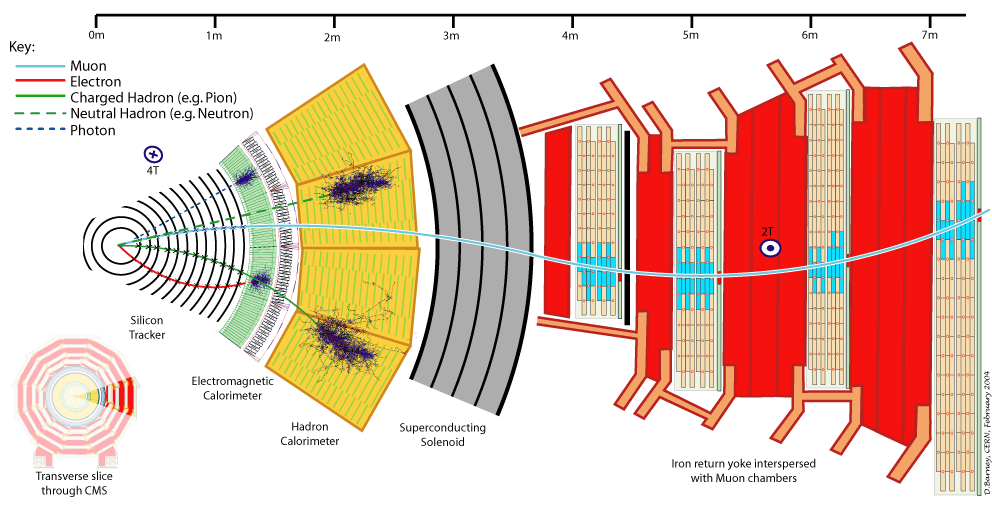
\includegraphics[width=0.75\textwidth]{assets/CMS_Slice.png}
\caption[CMS Detector Slice]{\textbf{Slice of the CMS detector.} The scheme shows the different detector systems as well as the tracks and the interactions of different particles with the detector. Source: \cite{cmsslice}}
\label{fig:ch_2_cmsslice}
\end{figure}

\subsection*{Coordinate System}
The origin of the coordinate system is chosen to be the intended collision point. The $z$ axis points in beam direction. The $x$ axis lies in the plane of the collider ring and points to its center. The $y$ axis points vertically upwards. The azimuthal angle $\phi$ is defined as the angle in the $x$-$y$ plane measured from the $x$-axis. The radial distance is $r = \sqrt{x^2 + y^2}$. The polar angle $\theta$ is measured from the $z$ axis. Another important quantity is the rapidity, which is a measure for the velocity of a particle and defined as
\begin{equation}
y = \textrm{artanh}\left(\frac{v}{c}\right) \quad ,
\end{equation}
where $v$ is the velocity of the particle and $c$ is the speed of light. $y$ is in contrast to $v$ unlimited and can take values in the range of $-\infty$ to $\infty$, further one can just add two rapidities together instead of using the relativistic valocity-addition formula. The pseudorapidity $\eta$ is a frequently used quantity in particle physics, in the relativistic approximation, $\eta$ is equal to $y$ and given by the equation
\begin{equation}
\eta = -\ln\left[\tan\left(\frac{\theta}{2}\right)\right] \quad ,
\end{equation}
which is used to denote the angle between a vector and the $z$ axis. A value of $\eta = 0$ is equal to $\theta = 90^{\circ}$; an angle of $\theta = 0^{\circ}$ equals $\eta = \infty$. The pseudorapidity is preferred over $\theta$ since the number of produced particles per $\eta$-interval is constant and the difference between two particles $\Delta\eta$ is invariant under lorentz boosts in $z$ direction. The momentum and energy of the initial partons is not determined in a hadron collider. Because of this, mainly the quantities transverse to the beam axis are of interest. These quantities, the transverse momentum \pt and the transverse energy \Et are invariant under lorentz boosts in $z$ direction. They are defined as 

\begin{equation}
\pt = \sqrt{p_{x}^2 + p_{y}^2} \quad \textrm{and} \quad \Et = \sqrt{E_x^2 + E_y^2} \quad .
\end{equation} 

Due to momentum conservation, the transverse momenta of all final particles sum up to zero. In the measurement there is always a missing amount of transverse momentum caused by gaps in the detector and neutrinos, which are not detectable within the CMS detector. The missing amount of transverse momentum is denoted as $p_\textrm{T}^{\textrm{miss}}$. 

\subsection*{Silicon Tracker}
Immediately after the collision, heavy objects are formed which decay after a short time and distance. The innermost part of the detector is of highest importance to reconstruct these objects and has to fulfill several requirements. First, a precise measurement of trajectories of charged particles is necessary to identify primary and secondary vertices. This also allows a momentum measurement as the full tracker is inside the superconducting solenoid, which produces a homogeneous magnetic field of 4\,T. Next, at each bunch crossing, about 1000 particles on average are created and travel through the detector. To distinguish these particles from each other and to assign the trajectories to the corresponding vertices, a high granularity is needed. Further, the time between two bunch crossings is about 25\,ns, therefore the response time and the cooling down period has to be short. Last, the detector components have to be resilient against this high amount of radiation.\\

To fulfill these requirements, silicon technology is used for the whole tracker system \cite{tracker}. When charged particles travel through these materials, electron-hole pairs are produced, which in turn generate an electric current in the read-out electronics. In the innermost part from $r=4.4$\,cm to 10.2\,cm, three barrel layers of pixel detectors are surrounding the beam axis. Each pixel detector has a size of 100\,$\times$\,150\,$\upmu \textrm{m}^2$. With this design, the desired impact parameter resolution is achieved. The pixel detectors are surrounded by ten layers of silicon micro-strip detectors up to a radius of 1.1\,m. As the particle flow decreases with the radius, larger detector elements can be used. This also reduces the amount of read-out electronics. The inner micro strip detectors have a size of 10\,$\textrm{cm}$\,$\times$\,80\,$\upmu \textrm{m}$, whereas the size of the outer ones is 25\,$\textrm{cm}$\,$\times$\,180\,$\upmu \textrm{m}$. 
At the endcaps, two disks of pixel detectors, three smaller and nine larger discs of strip detectors are installed. This allows a reconstruction of charged particle tracks up to $|\eta| < 2.5$. In total, the silicon tracker has a length of 5.8\,m with a diameter of 2.5\,m. At each bunch crossing, the occupancy of the detectors is at about 2-3\% for the inner micro strip detectors and 1\% or lower for the other ones. The track resolutions for charged particles of $1\,\GeV < \pt < 10\,\GeV$ and $|\eta| < 1.4$ are typically 1.5\% in \pt, 25--90 \mum in the transverse and 45--150 \mum in the longitudinal impact parameter \cite{trackerPerformance}.


\subsection*{Electromagnetic Calorimeter}
The electromagnetic calorimeter (ECAL) \cite{ECAL} surrounds the silicon tracker system hermetically and measures the energy of electrons, positrons and photons. Other electromagnetically interacting particles leave tracks but are not fully absorbed in the ECAL. The ECAL consists of several elements, the pseudorapidity interval up to $|\eta|<1.48$ is covered bu the barrel part while the endcap has a coverage of $1.48 < |\eta| < 3 $. The ECAL consists of homogeneous lead tungstate ($\textrm{PbWO}_4$) crystals which is the absorber and scintillator material at the same time. When electromagnetically interacting particles propagate through it, they produce photons through bremsstrahlung, which in turn create electron-positron pairs through pair production. An electromagnetic shower emerges. When the energy of the electrons drops to a critical amount, they mainly excite the atoms, which emit photons with characteristic wavelengths between 360\,\nm to 570\,\nm. This process is called scintillation. The photons are then measured with photomultipliers. The number of photons is proportional to the deposited energy of the particle. The radiation length of $\textrm{PbWO}_4$ is $X_0=0.89$\,cm. This means that after this distance, the energy of an electron or positron is reduced on average by the factor of 1/e. Moreover a photon has an average free path length of $9/7$ $X_0$ before it undergoes a process of pair production. The thickness of the ECAL with 23\,cm is equivalent to 25.8 $X_0$, therefore all electrons, positrons and photons are absorbed completely. \\

The ECAL was designed to measure the H $\rightarrow \upgamma \upgamma$ decay as precise as possible. Therefore, it provides a good energy resolution. To identify the background in this decay channel, a preshower detector is installed between the tracker and the ECAL. This element helps to identify neutral pions that decay into two photons; it also improves the position determination of electrons, positrons and photons. 

\subsection*{Hadron Calorimeter}
Hadrons propagate through the ECAL losing only a small fraction of their energy. Therefore, a hadron calorimeter (HCAL) \cite{HCAL} surrounds the ECAL, which absorbs all hadrons and measures their energy. The HCAL is important for measuring the properties of hadron jets as well as the total energy of the collisions and the resulting missing transverse energy. Several elements allow to measure forward jets up to $|\eta| = 5.2$. \\

The HCAL is a sampling calorimeter which exists of alternating absorbing layers and scintillating layers. The absorbing layer consists of brass and has a nuclear interaction length of $\lambda_\textrm{I} = $16.42\,cm. This is the mean distance for a hadronic particle after which it undergoes an inelastic nuclear interaction. Similar to the ECAL, a chain reaction starts and a hadronic shower emerges. As the HCAL is located inside the solenoid, its size is limited. The total absorber material of ECAL and HCAL makes up less than 7 $\lambda_\textrm{I}$. For hadrons that are not fully absorbed, an additional outer hadron calorimeter is installed outside the solenoid.
For the scintillating layers, plastic is used. When the hadronic shower hits these layers, the scintillator material gets excited and photons with characteristic wavelengths are emitted. They are guided through optical cables and measured by photodiodes.

\subsection*{Muon Detector}
The muon detector \cite{MuonChamber} is the outermost part of the CMS detector and covers the pseudorapidity interval of $|\eta| < 2.4$ without any gaps. The only particles that reach this part of the detector are neutrinos, which cannot be detected directly with the CMS detector, and muons. Muons have a high mass and are often high energetic. Because of this, they lose only small parts of their energy by propagating through the inner parts and are usually not fully absorbed in the muon detector. Muon identification and position determination is done with gaseous detectors. As they pass through these detectors, muons are ionizing the gas atoms. The resulting electrons and ions can then be measured as an electric current. The muon system consists of an iron return joke to guide the magnetic field lines of the solenoid through this part of the detector. This creates a magnetic field of 2\,T. As a consequence, muons travel a circular path. The momentum can then be determined by measuring the radius of its track. 

\subsection*{Trigger System}
The LHC has a bunch crossing rate of about 40\,MHz at each interaction point. This huge amount of data makes it impossible to store every event. Since interesting processes typically have low rates, it is sufficient for most analyses to store only a small fraction of promising events. To perform this data reduction, a trigger system \cite{TriggerDesignRep} consisting of two filtering steps is used at the CMS detector.\\

 The first filter is called the Level-1 (L1) trigger and is realized by hardware electronics. It decides in a few $\upmu$s whether it is worth keeping an event. In this short time, only a part of the information from the calorimeters and the muon chamber can be used. The trigger checks if the information is consistent with a physics object like an electron or a muon. This procedure reduces the event rate to less than 100\,MHz. \\

The second filter step is done by the High-Level Trigger (HLT). The HLT is realized with software tools where complex calculations and a more precise reconstruction can be done. In addition, the information of the tracking system is now included. This trigger reduces the event rate further to less than 1.5\,KHz. These events are then stored offline for more detailed analyses. 

\chapter{Simulation and Reconstuction of Events}
\label{ch:sim_reco}

%\section{Proton-Proton Scattering}
%In a proton-proton scattering process, different outcomes are possible. The cross section for one specific outcome is %proportional to the probability that this outcome will happen. The determination of the cross section $\sigma$ can be done in %multiple steps, for example for the top quark pair production with quarks one gets
%\begin{equation}\label{eq:ch_3_ppscatter}
%\sigma_{qq \rightarrow \textrm{t} \bar{\textrm{t}}} = \underbrace{\sum_{j,k}\int \textrm{d}x_j \textrm{d}x_k}_\text{sum initial states} \overbrace{f_j(x_j,\mu^2) f_k(x_k,\mu^2) }^\text{parton distribution functions} \ \underbrace{\hat{\sigma}(q_j q_k \rightarrow \textrm{t} \bar{\textrm{t}})}_\text{hard scattering process}\  \otimes \  \textrm{hadronization} \quad .
%\end{equation}
%First one has to sum over all initial states, a parton distribution function gives the probability to find a certain particle. The hard scattering process describes the transitions from the initial particles to the final state and the hadronization forms color neutral objects. In this section these steps will be described in more detail. 

All the available information about a particle collision is the measured deposited energy of each detector component. Together with some results of the online reconstruction e.g. trigger signals, this information is stored for further reconstruction. In the offline reconstruction, physical objects like electrons and hadrons are reconstructed. To compare the measured data with the theory prediction, or to investigate the efficiencies and robustness of algorithms, a simulation is needed. In this chapter the simulation process is described followed by an explanation of the reconstruction process. Additionally, methods to correct differences between the measured data, shortly denoted as data, and the simulation are summarized. 


\section{Event Simulation}
The simulation is done using as much theory input as possible. In the same order as the physical process, from the proton-proton scattering to the outgoing particles, one propagates the simulation. Due to insufficient theoretical descriptions, phenomenological models are used when necessary. After the outgoing particles are generated, the interaction with the detector materials is simulated. The emulation for the readout electronics generates signals that have the same signature as the data. 

\subsection{Proton-Proton Scattering}
A proton-proton scattering process leads to the production of a specific final state. The cross section is proportional to the probability to produce this final state. The determination of the cross section $\sigma$ is done in multiple steps, these steps are outlined in figure \ref{fig:ch_3_scattering} and explained in the following.

%FIXME plot zu proton-proton scattering like Husemanns
\begin{figure}
\centering
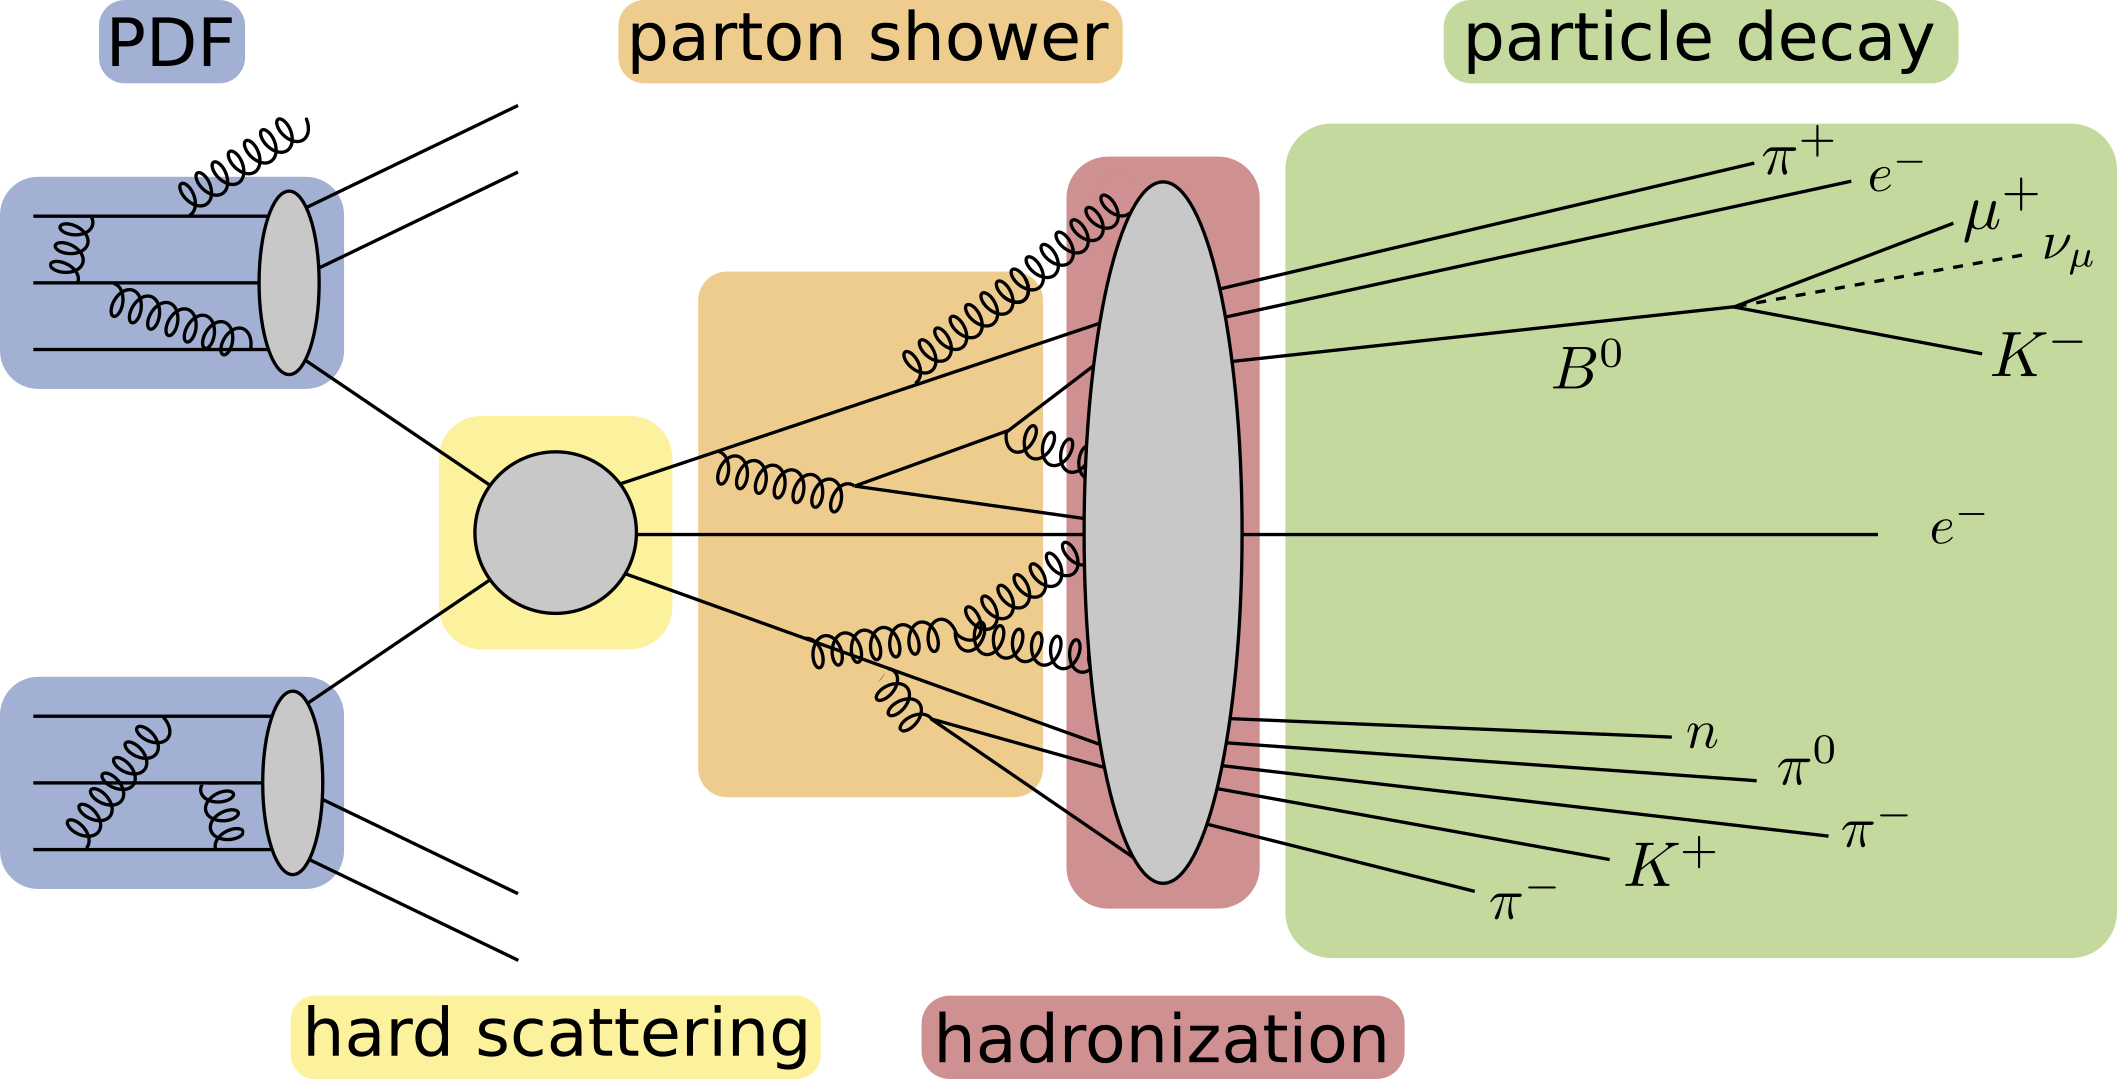
\includegraphics[width=0.8\textwidth]{assets/scattering.png}
\caption[Proton-Proton Scattering Process]{\textbf{Proton-proton scattering process:} The parton distribution functions (PDF) describe how the constituents of the proton are distributed. The deep inelastic scattering process of two elementary particles is calculated in the hard scattering. The subsequent processes are the parton shower, the hadronization and the particle decay.}
\label{fig:ch_3_scattering}
\end{figure}

\subsubsection*{Parton Distribution Functions}
As described in section \ref{sec:ch_1_QCD}, the proton is not an elementary particle but consists of so called partons. The valence quarks (uud) determine the quantum numbers of the proton. Apart from these, also gluons exist inside of protons as they are the exchange particles of the strong interaction. The gluons can split into virtual quark-antiquark-pairs; these quarks are the so called sea quarks. In a deep inelastic proton-proton scattering, two partons from two colliding protons interact with each other. Each parton carries a momentum fraction $x$ of the proton. The probability that a specific parton interacts, depends on $x$ and the absolute transfered momentum $Q$. It is given by a parton distribution function (PDF). As the PDFs cannot be computed by perturbation theory, they are determined by global fits to data from electron-proton scattering, fixed target experiments or hadron colliders. A classic approach is a polynomial ansatz for a specific PDF \cite{pdfOld}. A more modern approach is using a three-layer feed-forward neural network with 37 parameters \cite{nnpdf}. One can define a factorization scale $\mu$ and absorb low energetic gluons into the PDF, thereby infrared divergences are avoided. The use of the Dokshitzer-Gribov-Lipatov-Altarelli-Parisi (DGLAP)-equations \cite{DGLAP1,DGLAP2,DGLAP3} allows the evolution of gluon and quark PDFs to a desired value of $Q$. The PDFs for two different values of $\mu$ are shown in figure \ref{fig:ch_3_pdfs}.

\begin{figure}
%\hfill
%\subfigure{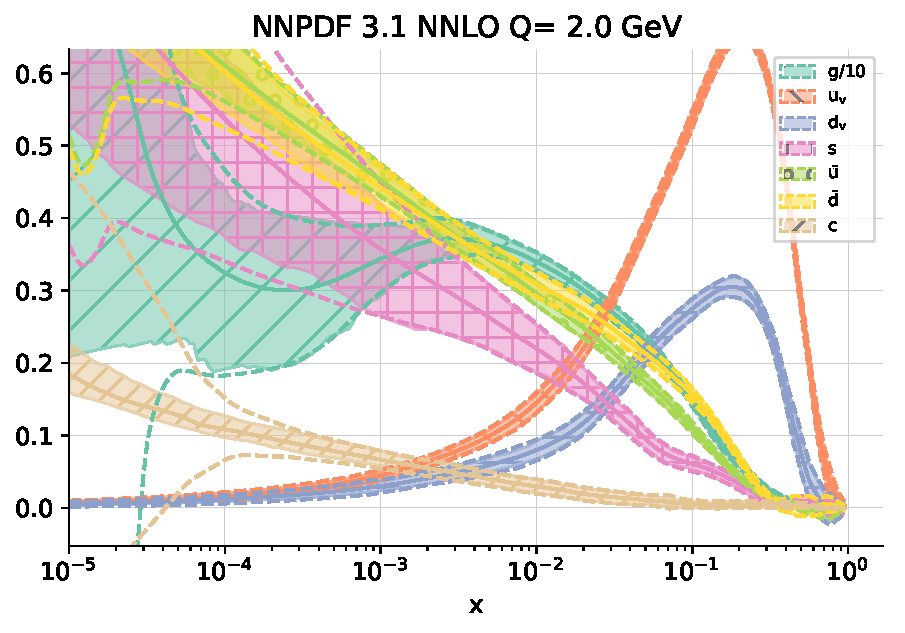
\includegraphics[width=7.25cm]{assets/NNPDF31NNLO_10GeV.pdf}}
%\hfill
%\subfigure{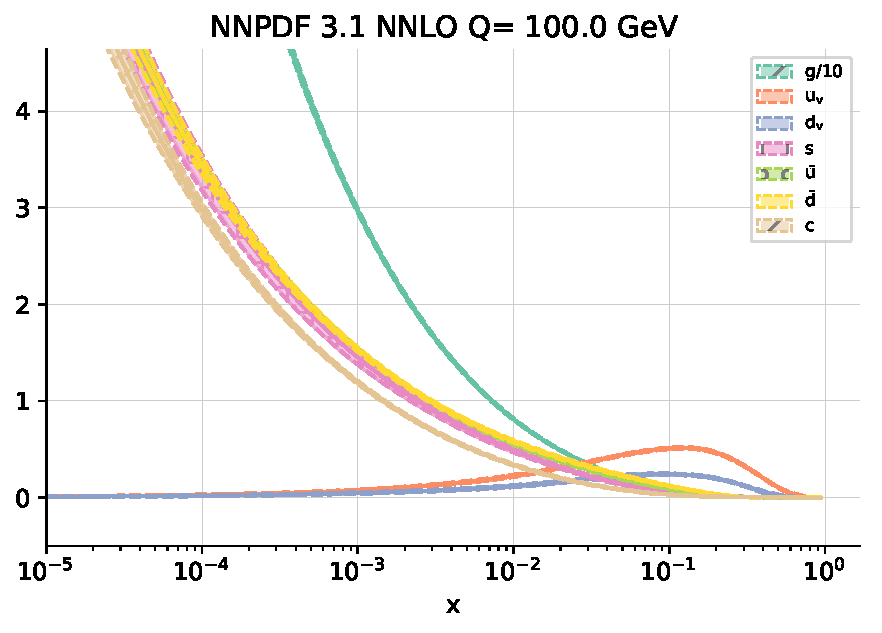
\includegraphics[width=7.25cm]{assets/NNPDF31NNLO_100GeV.pdf}}
%\hfill
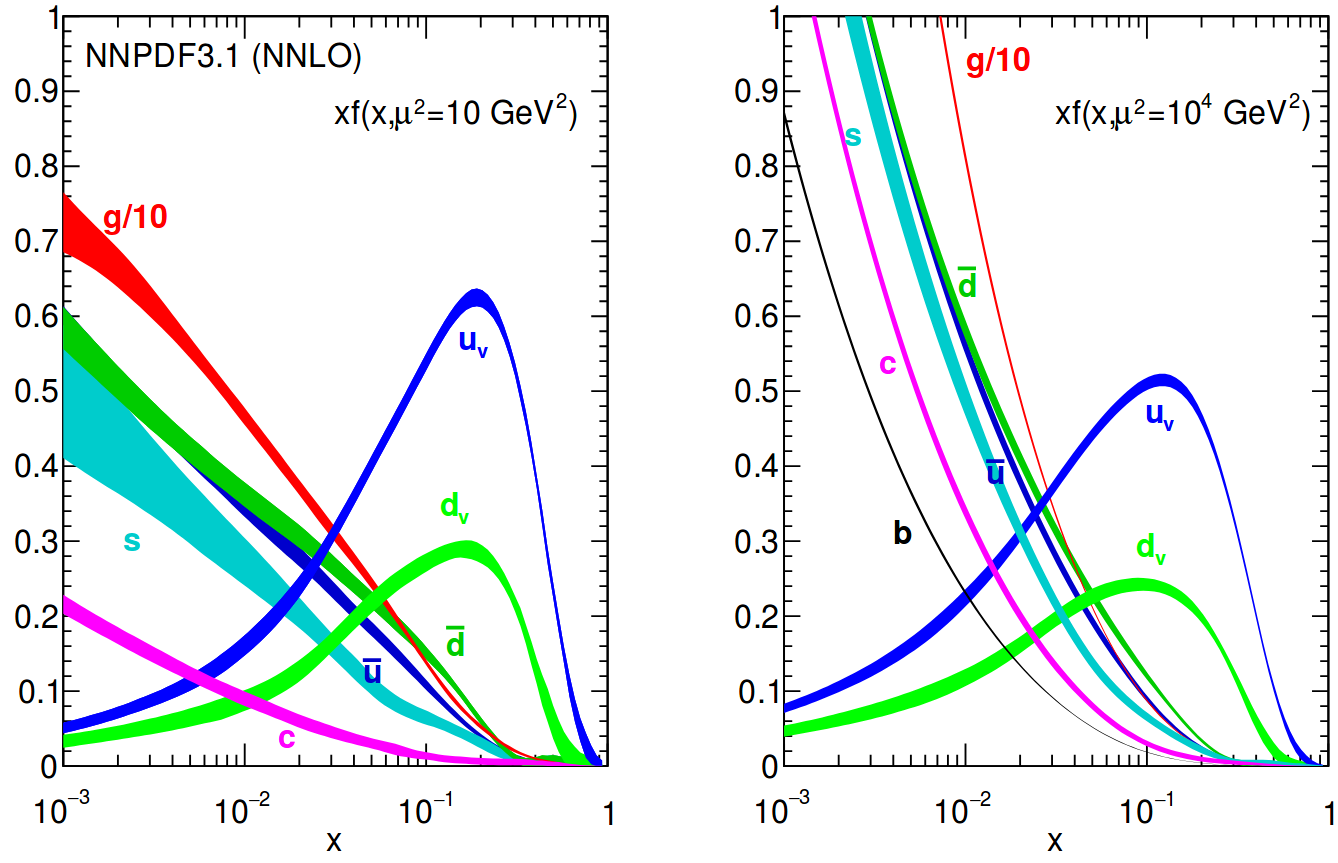
\includegraphics[width=0.75\textwidth]{assets/nnpdfs.png}
\caption[Parton Distribution Functions]{\textbf{Neural Network Parton Distribution Functions (NNPDFs).} Shown are the PDFs of gluons, valence quarks and sea quarks for different momentum fractions $x$ of the proton momentum. At lower values of the factorization scale (left) the valence quarks carry the majority of the proton momentum. At higher values of factorization scale (right) gluons carry the dominant part. The PDFs are computed using the DGLAP-equations in next-to-next-to-leading-order (NNLO). Source: \cite{nnpdf}}
   \label{fig:ch_3_pdfs}
\end{figure}

\subsubsection*{Hard Scattering Process}
The differential cross section $\textrm{d}\sigma$ for the hard scattering process is weighted with the PDFs $f_{i,j}$, which give the probabilities to find certain partons with certain momentum fractions $x$ and $y$ of the colliding protons. It is given by
\begin{equation} \label{eq:ch_3_sigma}
\textrm{d}\sigma = \frac{1}{3}\ \sum_{i,j}\ f_i(x,\mu^2)\ f_j(y,\mu^2)\ \frac{1}{2(xys)^2}\ |\mathcal{M}_{i,j \rightarrow \textrm{final}}|\ \frac{\textrm{d} \cos \theta\ \textrm{d}\phi\ \textrm{d}x\ \textrm{d}y}{8(2\uppi)^2} \quad ,
\end{equation}
with the square of the center-of-mass energy $s$ and the transition amplitude $\mathcal{M}_{i,j \rightarrow \textrm{final}}$ for an initial state to a final state, the so called matrix element. $\mathcal{M}_{i,j \rightarrow \textrm{final}}$ is obtained by summing up all Feynman diagrams for a specific process in a perturbation series. This is possible because the momentum of the partons is in a regime where $\alpha_s \ll 1$ and convergence of the series is given. Often it is sufficient to take the leading order (LO) Feynman diagrams, which are the ones with the minimal amount of vertices that are needed for a specific process. Including next-to-leading order (NLO) Feynman diagrams improves the accuracy of the simulation but is more complex and computationally intensive in generation.\\

The simulation is done with the help of Monte Carlo (MC) methods \cite{MCmethod}. MC methods can be used for numerical integration of higher dimensional phase spaces. In principle, to obtain one simulated event that obeys equation \ref{eq:ch_3_sigma}, the following can be done \cite[p. 48]{PPscattering}. Uniform distributed random numbers ($\theta,\ \phi,\ x,\ y,\ i,\ j$) are taken in the corresponding value ranges and $\left<\mathrm{d}\sigma\right>$ is calculated at one specific phase space point. The event is further processed if another uniform distributed random number $g$ in the range 0 < $g$ < $\mathrm{d}\sigma_\textrm{max}$ is lower than $\left<\mathrm{d}\sigma\right>$, where $\mathrm{d}\sigma_\textrm{max}$ is the supremum of $\mathrm{d}\sigma$. Otherwise it is discarded. Repeating this procedure equals an integration of the total phase space of equation \ref{eq:ch_3_sigma}.\\


\subsubsection*{Parton Shower, Hadronization and Particle Decay}
In addition to the final state particles of the hard scattering process, gluons and photons can be produced in initial or final state radiation. Gluons can radiate off another gluon or split into quark-antiquark pairs; photons can split into fermion pairs. These processes can recur and are described by the DGLAP-equations. A so called parton shower emerges. Because of the confinement (section \ref{sec:ch_1_QCD}), the partons form hadrons. This process cannot be described in a perturbation series as the assumption of $\alpha_s \ll 1$ does not hold for lower energies of the partons. The effect is described by phenomenological models like the Lund string model \cite{LundString}. The hadrons can further decay, as most of them are unstable. 

\subsubsection*{Underlying Event and Pileup}
Besides the hard scattering process of two partons, the remaining partons can interact themselves, producing additional signals in the detector at the same time. This effect is called underlying event. In the same bunch crossing, several other proton pairs are interacting with each other, this is called in-time pileup. Out-of-time pileup considers previous bunch crossings. The pileup distribution depends on the collider's properties. The more protons are in one bunch and the more focused the beams are, the more pileup events happen. In the data recorded in 2016, there were in average about 27 pileup events per bunch crossing in the CMS detector \cite{lhclumi2016}. The pileup events can be simulated as additional random scatterings and merged with the main event. 

\subsection{Simulation Tools} \label{sec:ch_3_simtools}
In the event simulation, several tools are used for the different steps. For the matrix element, one common generator is \textsc{MadGraph5} \cite{MadGraph5}. It sums up all Feynman diagrams in LO for given initial and final state particles. The matrix element is generated but not evaluated yet. The evaluation is done with the \textsc{MadEvent} package \cite{MadEvent} at given phase space points with the MC method and the cross section is calculated. For this reason a simulated event is often called MC event. \\

\textsc{MadGraph5}\textunderscore \textsc{aMC@NLO} \cite{MadGraph5_NLO}  is a further developement of \textsc{MadGraph5}, combining the features of MadGraph5 with the ones of \textsc{aMC@NLO}, where \textsc{aMC@NLO} can generate matrix elements at NLO in QCD. These tools also provide different parton-shower matching schemes to combine the final state particles with the parton shower. The parton shower itself has to be added with a parton shower simulation tool. As explained earlier, the parton shower can cause additional gluons in the final state, but such gluons can also be produced in NLO matrix element generators. To avoid double counting, the parts of the parton shower that match the NLO Feynman diagrams are subtracted. This is implemented by using negative event weights.\\

Another matrix element generator that includes Feynman diagrams up to NLO in QCD is \textsc{Powheg} \cite{Powheg1, Powheg2, Powheg3}. \textsc{Powheg} uses a different method than \textsc{aMC@NLO} to avoid double counting and negative event weights. It demands a parton shower simulation that generates the emission with the highest \pt first and then corrects the NLO emission. \\

\textsc{Pythia} \cite{Pythia82} is a general purpose tool for the simulation of the hard process as well as the parton shower, the hadronization, the particle decay and the underlying event. The hard process is only calculated in LO, but \textsc{Pythia} provides several interfaces to external programs. Therefore, the matrix element generators explained above can be used in combination with \textsc{Pythia}. \\

To be able to compare simulation with data, the detector response has to be simulated as well. This is done with the \textsc{GEANT4}\cite{Geant4} toolkit. In \textsc{GEANT4}, the different materials of the detector system, including dead materials, are modeled. The particles are propagated through these materials while taking into account the effect of the magnetic field on charged particles. Interactions like bremsstrahlung, multiple scattering and photon pair-production are simulated. The generated signals in the active detector materials are taken as input for emulators of readout electronics and trigger systems. After this step, the detector information of a simulated event is in the same manner as for data. To get the best comparison between data and simulation, the event reconstruction of the detector signals is done in the same way as for data. This will be subject of the next section.


\section{Event Reconstruction}
In this chapter, the aim to reconstruct physics objects out of the measured or simulated detector information is described. In a first step of the event reconstruction, particle tracks and the corresponding interaction points, called vertices, are reconstructed. In several subsequent steps, the identification and reconstruction of particles that penetrate the detector is done. These are electrons, muons, photons, charged hadrons, neutral hadrons and neutrinos. Afterwards, adjacent particles are bundled to so called jets. 

\subsection{Tracks and Vertices}
Tracks of charged particles are reconstructed from the tracker information. Therefore, tracker hits are created from clustering signals of the silicon pixel and strip detectors. The tracks are produced using an iterative track finding algorithm. From tracker hits in the inside of the detector, where the occupancy of each detector element is low, tracker seeds are created. The track finding is performed with the Kalman filter approach \cite{KalmanFilter}. In the first iteration step, the seeds have tight constrains. This gives only a moderate efficiency, but also a minimal fake rate. The energy deposits of the corresponding hits are then removed, which simplifies the track finding problem. At the next iteration step with looser seeding criteria, a higher efficiency is achieved. Repeating this, one gets an efficiency to find isolated muons of 99.5\% and more than 90\% to find charged hadrons while the fake rate is of about 1\% \cite{ParticleFlow2}. Each track has several quality criteria like the number of hits, a normalized $\upchi^2$ value and the compatibility to a certain vertex.\\

Because of pileup, there exists more than one vertex for each event. The vertex from where the hard scattering originates is the primary vertex (PI), it has to be identified in order to remove the tracks originating from pileup. The vertex reconstruction starts with a set of possible vertices and each track is extrapolated to a point $z_i$ on the beam line. For each track and vertex pair a probability $c_{ik}$ is estimated that the track is originating from the regarded vertex. A $\upchi^2$ function, weighted with these probabilities
\begin{equation}
\chi^2 = \sum_{i,k} c_{ik} \frac{(z_i-z_k)^2}{\sigma_i^2}	\quad ,	
\end{equation}
is minimized to determine the exact position of the vertices $z_k$. As the probability depends on the vertex position, an iterative procedure is used. After a final selection, a set of vertices is obtained. The primary vertex is selected as the one with the highest sum of $p_\textrm{T}^2$ of its tracks. 

\subsection{Particle Reconstruction}
For reconstructing particles as precise as possible, the combination of all subdetectors is used within the particle flow (PF) algorithm \cite{ParticleFlow, ParticleFlow2}. The identification of PF candidates, namely electrons, muons, photons, charged hadrons and neutral hadrons is explained in the following. 

\subsubsection*{Calorimeter Clustering}
The tracker system gives the most precise information about the position and through the curvature of the track, it gives also the best determination of the momentum of charged particles. The calorimeters support the determination of the energy and direction of charged particles in cases of high \pt or low quality tracks. Moreover the energy and direction of photons and neutral hadrons is measured while the contributions of charged particles are separated. This is done in the calorimeter clustering process, where each calorimeter element, the ECAL barrel, the ECAL endcap and the several HCAL elements, are handled separately. The process starts on calorimeter cells with a local maximum of deposited energy. Then, adjacent cells are combined, if their deposited energy exceeds a certain threshold. For each calorimeter element, one can have several calorimeter clusters. Together with the charged-particle tracks and the muon tracks, PF elements can be constructed.

\subsubsection*{Electrons}
An electron is identified if a charged-particle track matches an ECAL cluster with a typical electron shower profile. A fit starting with a track seed is combining both signals and the momentum is determined. A complimentary algorithm for electrons with high \pt starts with taking a seed from the ECAL. In this algorithm, several ECAL clusters are combined to so called ECAL superclusters which have a characteristic form for electrons \ref{ERec}. The quality of an electron fit is described by several quantities like the matching of the track to the cluster or the distance of the track to the primary vertex. A tight requirement on these quantities can lower the fake rate.

\subsubsection*{Muons}
For the muon reconstruction, tracks in the muon chamber are computed in a similar way as in the tracker. These muon tracks are propagated towards the beam line and combined if possible with the most suitable track of the inner tracker. A refit using the information of both sub detectors gives an improved muon track. A reconstruction process for low \pt muons that do not create a muon track, starts with propagating an inner tracker track and tries to find a minimal muon information in the muon tracker. Again one can choose looser or tighter demands on muon tracks afterwards to further reduce the fake rate.

\subsubsection*{Hadrons and Photons}
For the reconstruction of charged hadrons, the energy depositions of clusters in ECAL and HCAL are compared to the momentum of the charged particle tracks. In case of an agreement with one or more tracks, a combined fit is performed. In case of disagreement, several scenarios including additional neutral hadrons or photons are considered. After all charged-particle tracks are matched to PF elements, their energy deposits are removed and neutral particles are identified. Neutral particles do not produce any hits in the tracker, therefore they have only bad direction information and an assignment to a vertex is not possible. Because of this, also neutral particles coming from pileup are included.

\subsection{Jet Reconstruction}
A jet is a particle shower of hadrons, leptons and photons that originates in the most cases from a single particle. There are different ways to reconstruct a jet, the default method used in the CMS experiment collects several nearby PF elements in a cone up to a given size in a sequential recombination process. This is done with the anti-$k_\textrm{t}$ jet clustering algorithm \cite{antikt}. \\

\begin{figure}
\centering
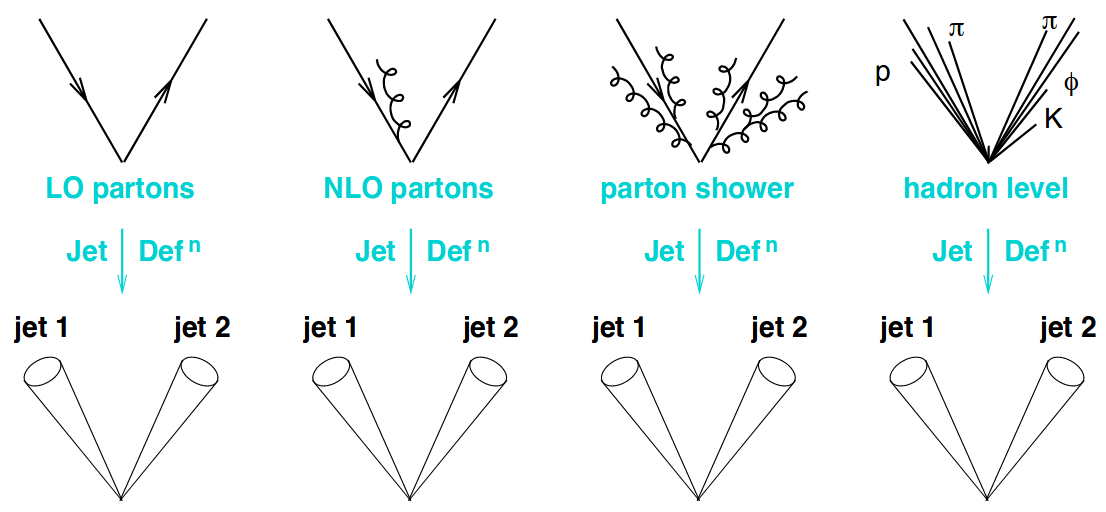
\includegraphics[width=0.75\textwidth]{assets/IRCsafety.png}
\caption[Infrared and Collinear Safety of Jets]{\textbf{Infrared and collinear safety.} A jet can be defined on different levels. In a theoretical description, it originates from one single particle and can therefore defined as this particle. In perturbation theory, several vector bosons can be radiated in addition. On the detector level, the jet is defined by color neutral objects. With an infrared and collinear safe jet clustering algorithm, the resulting jets are independent of the level of definition. Source: \cite{ICLsafe}}
\label{fig:ch_3_IRCsafety}
\end{figure}

An advantage of this algorithm is its infrared and collinear safety. This means, that the same jet is found with and without a soft or collinear radiation, for example a gluon radiation or a gluon splitting. Therefore, this algorithm is independent of the technical level of the jet definition as shown in figure \ref{fig:ch_3_IRCsafety}. For the clustering process, a distance measure $d_{ij}$ between two particles $i$ and $j$ is defined as
\begin{equation}
d_{ij} = \textrm{min}(k_{\textrm{t},i}^{-2},k_{\textrm{t},j}^{-2})\frac{\Delta R^2_{ij}}{R^2} \quad ,
\end{equation}
where $k_{\textrm{t},i}$ is the momentum of a particle, $R^2 = (y^2 + \phi^2)$ is the radius in the $y$-$\phi$ plane with the rapidity $y$ and $\Delta R^2_{ij} = (y_i - y_j)^2 + (\phi_i - \phi_j)^2$ is a radial distance of two particles. A distance measure $ d_{i\textrm{B}}$ between a particle $i$ and the beam axis is defined as
\begin{equation}
d_{i\textrm{B}} = k^{-2}_{\textrm{t},i} \quad .
\end{equation}
For the general jet reconstruction of data taken from run 2 of the CMS experiment, a radius of $R=0.4$ was chosen. In the sequential recombination algorithm, all possible $d_{ij}$ are computed and two particles with the smallest $d_{ij}$ are combined to new pseudo-particles. This is repeated until $d_{i\textrm{B}}$ is the smallest distance. The remaining pseudo-particles become then the jets. In this way, the hardest particles (the ones with the highest \pt) are combined with nearby soft particles (the ones with low \pt). If the cones of two hard particles overlap, they share the softest particles and create two separate jets with partial cones. 

\subsection{Lepton Isolation}\label{sec:ch_3:Isolation}
Muons and electrons often appear inside of QCD jets originating from b, c or s quark decays. Isolated leptons on the other hand appear often in rare processes, they are good indicators for leptonic top quark decays ($ \textrm{t} \rightarrow \textrm{b} + \upnu_l + l^+$). Therefore an isolation criteria is useful to find events with bottom quarks without directly looking at them. An isolation can be described using the momenta and energies $p_\textrm{T}^\textrm{charged}$, $E_\textrm{T}^\textrm{neutral}$ and $E_\textrm{T}^\upgamma$ of the PF elements for the charged particles, the neutral particles and the photons respectively inside a cone of 
\begin{equation}
\Delta R = \sqrt{\Delta\eta^2 + \Delta\phi^2} = 0.4 \quad .
\end{equation}
Since the tauon decays in the beam line, only for an electron or a muon with its momentum $p_\textrm{T}^l$ an isolation can be defined as
\begin{equation}
I_l^{\textrm{PF}/\Delta \upbeta} = \frac{\sum p_\textrm{T}^\textrm{charged} + \textrm{max} \left(0.0, E_\textrm{T}^\textrm{neutral} + \sum E_\textrm{T}^\upgamma - 0.5 \sum E_\textrm{T}^\textrm{charged}(\textrm{PU})\right) }{p_\textrm{T}^l} \quad .
\end{equation}
The so called $\Delta \upbeta$ correction is included where contributions of the neutral particles from pileup interactions are subtracted. They are estimated as half of the energy coming from charged particles in pileup $\sum E_\textrm{T}^\textrm{charged}(\textrm{PU})$. A lower value of $I_l^{\textrm{PF}/\Delta \upbeta}$ corresponds to a more isolated electron or muon.  


\subsection{Reconstruction of Neutrinos and Leptonically Decaying W Bosons}
At the LHC, the transverse momentum $\vec{p}_\textrm{T} = (p_x, p_y)^\textrm{T}$ of the colliding particles is zero, therefore the sum of the $\vec{p}_\textrm{T}$ of all generated particles after the collision has to be zero as well. As neutrinos cannot be measured within the CMS detector the missing part of the transverse momentum can be attributed to neutrinos. For historical reasons and as the momentum is equal to the energy in the relativistic regime using natural units, the missing part is denoted as the missing transverse energy 
\begin{equation}
\vec{\slashed{E}}_T = - \sum_i \vec{p}_{\textrm{T},i} \quad .
\end{equation}
Decays of the W boson into a charged lepton and a neutrino are called leptonic W boson decays. With the measured $\vec{\slashed{E}}_T$ and the momentum of the lepton, the transverse mass of the W boson $m_{\textrm{T,W}}$ can be reconstructed 
\begin{equation}
m_{\textrm{T,W}} = \sqrt{(\vec{p}_{\textrm{T},l} + \vec{p}_{\textrm{T},\nu})^2 - (p_{x,l} + p_{x,\nu})^2 - (p_{y,l} + p_{y,\nu})^2} \quad ,
\end{equation}
with $\vec{p}_{\textrm{T},\nu}$ the neutrino momentum set to $\vec{\slashed{E}}_T $. This method allows to reconstruct the W boson if there are no additional W bosons or leptons in the event.

\section{Differences between Data and Simulation} \label{sec:ch_3_Reweighting}
As mentioned before, the simulation is not exact since in each step smaller or larger inaccuracies are made. These differences lead to discrepancies between data and simulation after the reconstruction. Several steps can be done to improve the agreement afterwards, these are explained in the following.

\subsection{Jet Energy Corrections}
In general, the measured jet energy does not match the true parton energy, where the jet originated from. One reason is pileup and underlying events. Due to the tracks, the charged particles from pileup can be removed reasonably well but the neutral particles not. Also neutrinos are not measured and they appear also in jets, therefore, their energy is missing. Moreover, there is a disagreement in data compared to simulation due to inaccuracies in the simulation. With jet energy corrections (JEC) \cite{JEC}, these differences are mitigated in several steps with some variation for data and simulation. These steps are outlined in figure \ref{fig:ch_3_JEC}.

\begin{figure}
\centering
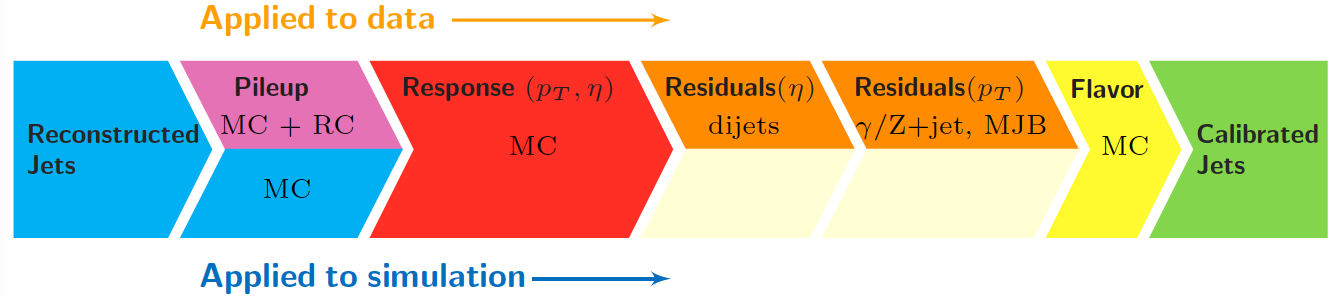
\includegraphics[width=0.95\textwidth]{assets/JEC_levels.png}
\caption[Jet Energy Corrections]{\textbf{Jet Energy Corrections.} In the first step, based on information from simulation, energy contributions from pileup and electronics noise are removed. In data, the residual differences between data and simulation as a function of $\eta$ is flattened as well. Next, the response of the detector is corrected. Therefore, the residual differences in simulation between the reconstructed \pt and $\eta$ and the corresponding true values are flattened out. The resulting correction is performed in data and simulation. A further step is done only on data, here small residual differences between data and simulation in \pt and $\eta$ are corrected. An optional last step is the correction in dependence of the flavor of the jet using the truth information from the simulation. Source: \cite{JEC_levels}}
\label{fig:ch_3_JEC}
\end{figure}

\subsection{Pileup Reweighting}
The simulation is done before or during the actual data taking period, therefore a pileup distribution has to be assumed in the simulation. To correct most of the disagreements caused by the different pileup interactions, the simulated events can be assigned with a weight in a way that the pileup distributions in data and simulation are equal. The pileup weights are given by 
\begin{equation}
w_{\textrm{PU},i} = \frac{n_{\textrm{data},i}}{n_{\textrm{MC},i}} \quad ,
\end{equation}
with the number of data events $n_{\textrm{data},i}$ and the number of simulated events $n_{\textrm{MC},i}$ in dependency of the number of primary vertices $i$. The pileup distributions for the 2016 data and simulation are shown in figure \ref{fig:ch_3_pup}. 

\begin{figure}
\centering
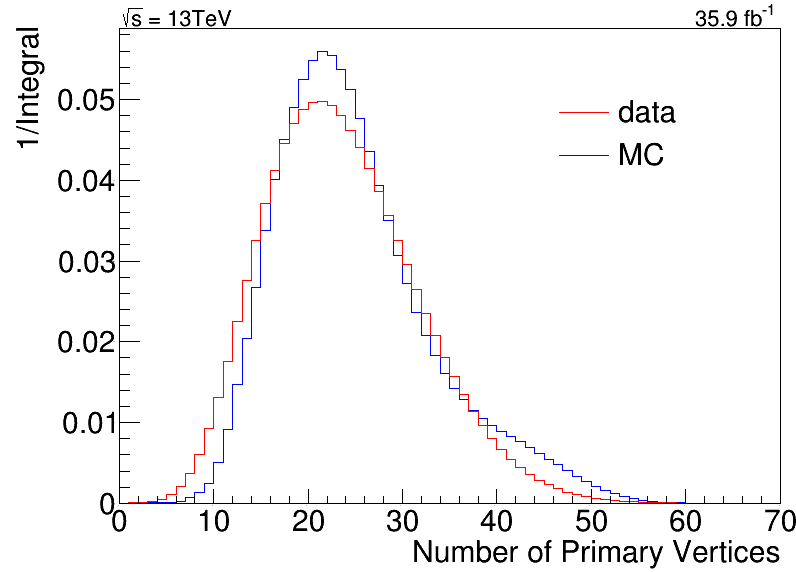
\includegraphics[width=0.5\textwidth]{assets/pup.png}
\caption[Pileup Distributions for Data and Simulation]{\textbf{Pileup distribution for data and simulation.} Shown is a normalized histogram of the events as a function of the number of primary vertices. In each bin where the data is above the simulation, the simulation gets up-weighted; when the data is lower than the simulation, the simulation gets down-weighted.}
\label{fig:ch_3_pup}
\end{figure}

\subsection{Trigger and Lepton Efficiencies}
The efficiency of the triggers is also different in data and simulation. In order to mitigate this discrepancy, scalefactors are used to correct the simulation
\begin{equation}
sf_\textrm{trigger} = \frac{\epsilon_\textrm{data}(\pt,\eta,\dots)}{\epsilon_\textrm{MC}(\pt,\eta,\dots)} \quad ,
\end{equation}
where the efficiencies $\epsilon_\textrm{data,MC}$ are functions of different quantities. For example a muon trigger has a strong dependency on the \pt of the corresponding muon. \\

Lepton scalefactors are needed whenever a selection of leptons is performed as the efficiencies of the identification of a lepton are different in data and simulation. The efficiencies are moreover dependent of the selection of the lepton, they are often separated for different parts of the selection (for example for the tracker selection and the isolation criteria) and can be combined. For some selection criteria, scalefactors are already measured.





\chapter{Artificial Neural Networks}
\label{ch:stat}
%Jets arise from hadronically decaying particles which are gluons, tauons and all quarks except top quarks. By investigating its shape and composition, a jet can be assigned to its most probable origin particle. This is a high dimensional classification problem where different methods have been used in the past. The statistical basics are outlined in this chapter. In the first section, the Neyman-Pearson-Lemma is described that gives theoretically best possible separation between two classes. In practical applications, neural networks achieve the best performance and are therefore outlined afterwards. Next, the concept of domain adaptation is explained that is the main content of this work and is used to 

%Consider various samples that belong to distinct statistical populations. Each population has characteristics which follow a probability distribution. For each element in a sample, the characteristics take on certain values. The values can be used to calculate the probability that an element origins from a specific population. This can only be done if the probability distribution is known, which is seldom the case. If for a sample the corresponding population is known, one can estimate the probability distribution for the given characteristics. \\

%The ANN can learn to approximate the probability distributions of several populations. It can map the elements with certain values of the characteristics to probabilities for specific populations. For the approximation, samples with the information of their corresponding population are needed. The process of learning the approximation is called training.\\

%\section{Neyman-Pearson-Lemma}

%Artificial neural networks (ANNs) are a class of algorithms inspired by the biological brain. ANNs are widely used in machine learning and pattern recognition. Similar to a biological neural network, an ANN consists of several connected artificial neurons. The connection between two neurons is called edge and transports the information, which is a single value. Each edge has a so called weight, this weight determines the importance of the corresponding value. Each neuron takes the values of the connected input edges and computes an output value that is transported via the output edges to other neurons. An ANN provides an interface in the form of input and output neurons. The input neurons are placeholders for values which are processed through the ANN. The output neurons provide their calculated output values. \\

%ANNs can learn to approximate multidimensional probability distributions in a process called training. In this thesis an ANN was used to assign jets to their initial particles. Jets from b quarks origin from other distributions than jets from c or light flavor quarks or gluons. Based on simulation, an ANN was trained to distinguish between these distributions. The specific type of ANN used in this thesis is called feed-forward multilayer perceptron. It is described in section \ref{sec:ch_4_mlp}.
%The core subject of this thesis is the domain adaptation as an extension of this ANN to improve its data to simulation agreement. The domain adaptation is described in section \ref{sec:ch_4_da}. A comprehensive introduction to machine learning techniques is provided in \cite{Bishop} or \cite{DeepLearningBook}. 

Artificial neural networks (ANNs) are a class of algorithms inspired by the biological brain and widely used in machine learning and pattern recognition. In this thesis, ANNs were used for a multivariate classification task, this problem is outlined in section \ref{sec:ch_4_classification}. ANNs consist of several artificial neurons, in section \ref{sec:ch_4_perceptron}, the functionality of a single artificial neuron is explained. In section \ref{sec:ch_4_mlp} the kind of ANN, used in this thesis is described. The core subject of this thesis is the domain adaptation as an extension of ANNs to improve its data to simulation agreement. The domain adaptation is described in section \ref{sec:ch_4_da}. A comprehensive introduction to machine learning techniques is provided in \cite{Bishop} or \cite{DeepLearningBook}. 

\section{Multivariate Classification}\label{sec:ch_4_classification}
In a multivariate classification task one tries to assign a data point with characteristic variables to one of several classes. If the distributions of the characteristic variables overlap for different classes, the data points are not completely separable. That means only the probability that one data point belongs to a certain class can be obtained. Consider two classes, denoted as class one and class two. From the output of a classifier, a so called test statistic can be constructed to separate the two classes. The test statistic can be chosen on a fixed value, all data points with a test statistic higher (lower) than this value are said to be class one (two). Due to the fact that the classes are not completely separable, not all data points can be classified correctly. Consider class one (two) as the signal (background) class. The efficiency is the fraction of data points of class one that are correctly classified. The false positive rate (FPR) is the fraction of class two data points that are mistakenly classified as class one. The closer the value of the efficiency is to 1 and the closer the FPR is to 0, the better the classifier.\\

The multivariate classification in this thesis is done with ANNs by constructing a function that maps an input vector $\vec{x}$ of characteristic variables (features) to an output vector $\vec{y}$ that describes the probabilities of the classes. An ANN has various free parameters. In a process called training, these parameters are adjusted to get a function with high efficiency and low FPR. The process of training is done using so called training samples. For each data point of these samples the corresponding class is known, therefore the $\vec{y}$ is labeled. 

\section{Perceptron} \label{sec:ch_4_perceptron}
\begin{figure}
\centering
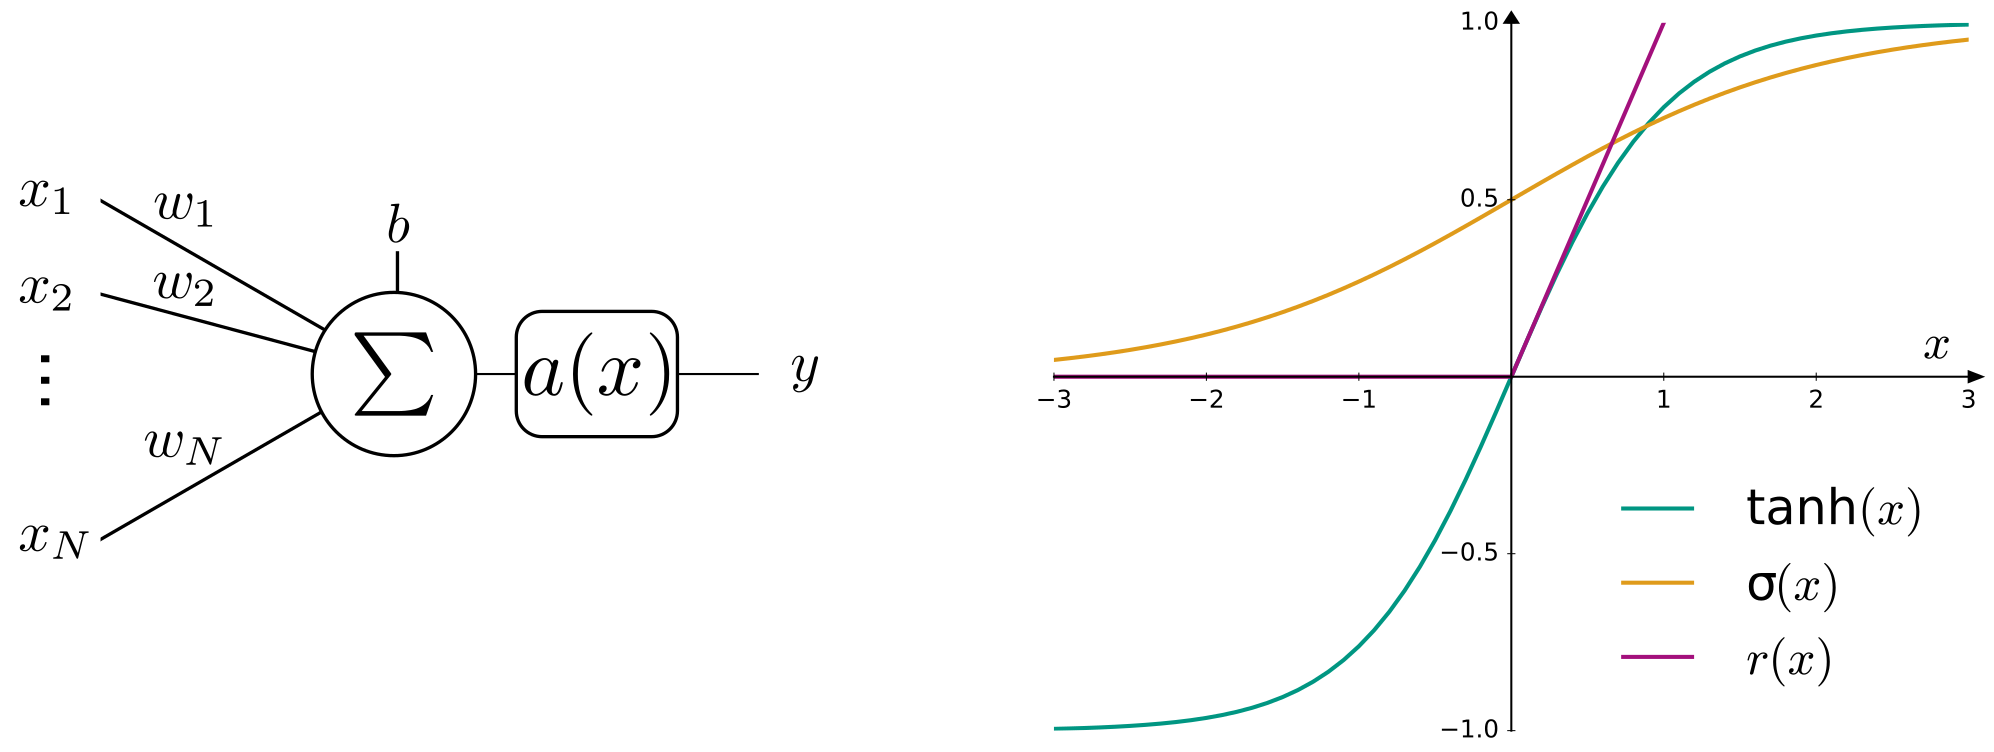
\includegraphics[width=0.8\textwidth]{assets/perceptronAndActivation.png}
\caption[Perceptron and Activation Function]{\textbf{Perceptron (left).} An ANN consisting of one neuron as shown on the left is called perceptron. Several neurons can be connected to a multilayer perceptron. \\
\textbf{Activation functions (right).} Three common activation functions are shown.}
\label{fig:ch_4_perceptron}
\end{figure}
One single neuron can be used to construct simple mathematical functions. The first was introduced by rosenblatt and is the rosenblatt perceptron. The computation is done by taking all input values $x_i$, multiplying them with adaptable weights $w_i$ and adding an adaptable bias $b$. The result is mapped by an activation function $a(x)$ to one single output value
\begin{equation}
y = a\left(\sum_i x_i w_i + b\right) \quad .
\end{equation}
Commonly used activation functions are the sigmoid function
\begin{equation}\label{eq:ch4_sigmoid}
\sigma(x) = \frac{1}{1+\exp(-x)}	\quad ,
\end{equation}
and the hyperbolic tangent $\tanh(x)$. However, these are problematic when applied to more complex neural networks \cite{VanishingGradientProblem}, therefore the rectifier activation function (ReLu) \cite{relu}
\begin{equation}\label{eq:ch4_relu}
r(x) = \max(0,x)	\quad ,
\end{equation}
is preferred for them. The perceptron and the mentioned activation functions are shown in figure \ref{fig:ch_4_perceptron}. This perceptron is able to solve linearly separable problems. For more complex problems, an ANN consisting of several neurons can be used.


\section{Multilayer Perceptron}\label{sec:ch_4_mlp}

A multilayer perceptron (MLP) is the standard type of ANN where several neurons are aligned in layers. An MLP can be further distinguished according to its architecture. The architecture describes the configuration of the MLP, it determines the number of layers, the number of neurons of each layer, how the neurons are connected among each other and the activation functions used. With the use of an appropriate architecture and training procedure, the output values can take on meaningful values. 

\subsection{Fully Connected Feed-Forward Networks}

\begin{figure}
\centering
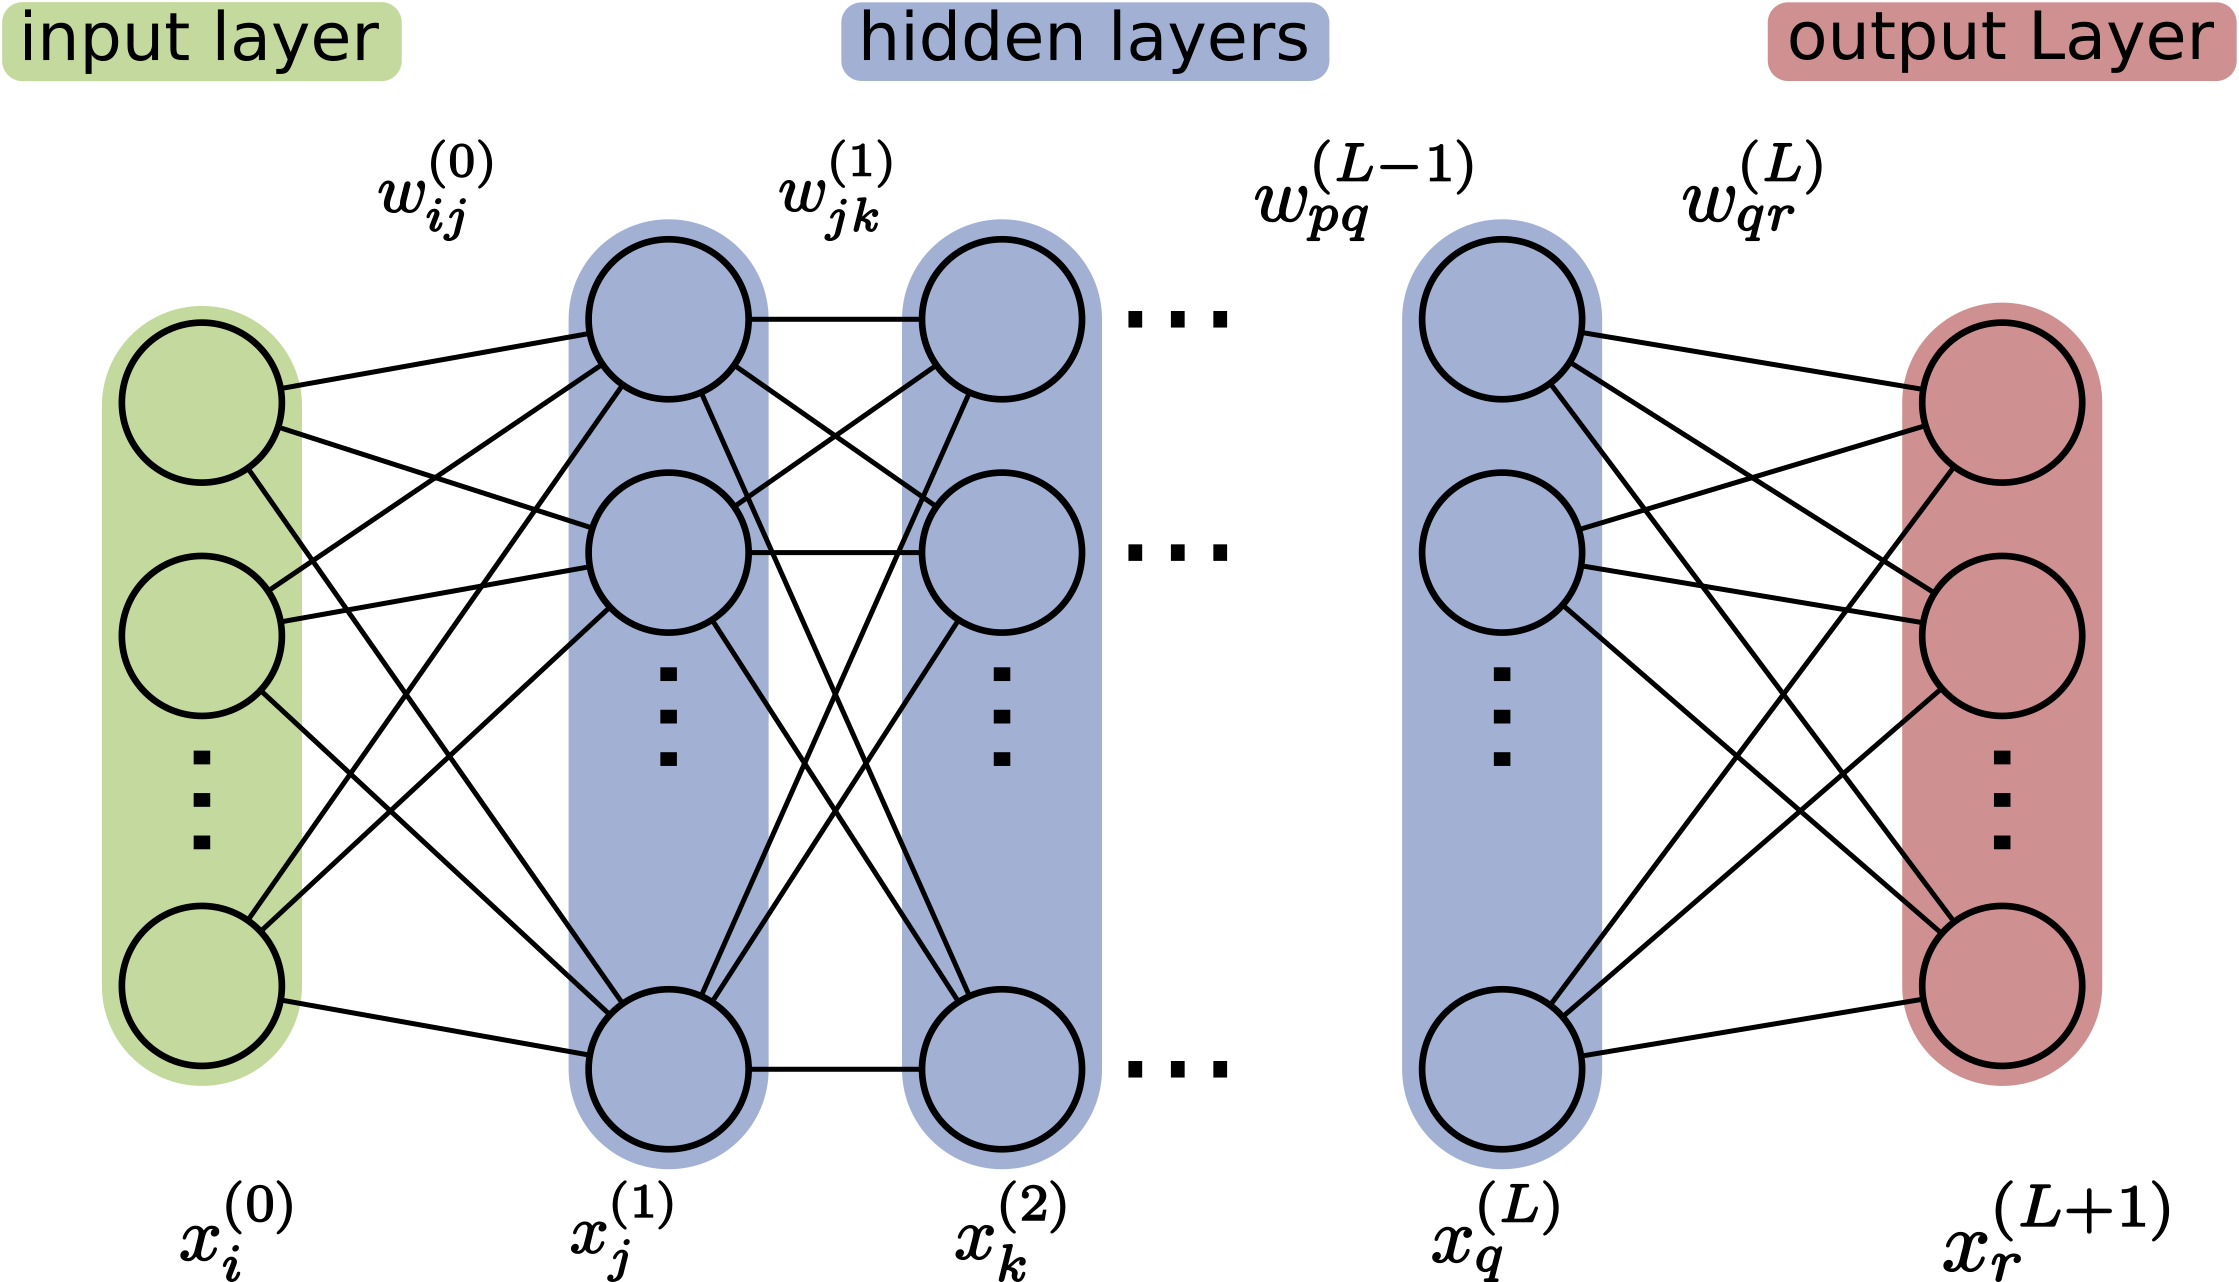
\includegraphics[width=0.8\textwidth]{assets/ann_3.png}
\caption[Multilayer Perceptron]{\textbf{A multilayer perceptron} with $L+2$ fully connected, feed-forward layers. The first layer (green) is called the input layer and the last layer (red) is called the output layer. In between there are $L$ layers (blue), referred to as hidden layers.  The circles represent the neurons while the connections between them are the edges. Each edge has a weight $w_{ij}$ where $i$ and $j$ indicate its source and target neuron respectively. Each neuron has a bias and delivers a value $x_i$, the biases are not shown.}
\label{fig:ch_4_dnn}
\end{figure}
If the MLP has a feed-forward structure, the connections between neurons do not form circles. If it is additionally fully connected, each neuron takes input values from all neurons of the preceding layer while the output values are connected to all neurons of the following layer. An example of a fully connected feed-forward MLP is shown in figure \ref{fig:ch_4_dnn}. The number of input and output neurons is determined by the number of features and classes of the specific multivariate classification task. The number of hidden layers and the number of neurons in each hidden layer can be chosen freely. These determine the number of free parameters, the biases and the weights. MLPs with more than one hidden layer are called deep neural networks (DNN). The output of an arbitrary neuron can be calculated recursively by 
\begin{equation}
x_i^{(k+1)} = a^{(k+1)}_i \left( \sum_{j=1}^{\ N^{(k)}} x_j^{(k)} w_{ij}^{(k)} + b_{i}^{(k)} \right) \quad ,  
\end{equation}
where $k$ denotes the layer and $N^{(k)}$ the number of neurons in this layer. As an activation function in the final layer, it is reasonable to use a softmax function
\begin{equation}\label{eq:ch4_NN_softmax}
y(\vec{x})_k = \frac{\exp(x_k)}{\sum_{j=1}^N \exp(x_j)}	\quad ,
\end{equation}
to normalize the sum of all output values to 1. With the presented architecture, the input values can be propagated through each layer and the output values can be calculated. This process is called forward propagation. 


\subsection{Training}\label{sec:ch_4_training}
The training is done by minimizing a function that takes the computed output values of the ANN for given training samples and measures the deviation from the corresponding labels. This function is called the error function, it calculates one single value, the so called loss.\\

Consider a binary classification problem where the ANN has one single output neuron with a sigmoid activation function. Moreover each element of the training sample has a label $l$ with $l=1$ for one class and $l=0$ for the other. An appropriate error function is the binary cross-entropy 
\begin{equation}\label{eq:ch4_bce}
E(\vec{x};\vec{w},\vec{b}) = - \sum_{n=1}^{N}\left( l_{n} \ln y_n + (1-l_n)\ln(1-y_n) \right)\quad ,
\end{equation}
where $n$ indicates the elements of the training sample and $y_n = y_n(\vec{x};\vec{w},\vec{b})$ the computed output value of the ANN. One can show that the binary cross-entropy together with the sigmoid activation function (equation \ref{eq:ch4_sigmoid}) is equivalent to the negative log likelihood function \cite[p. 234-236]{Bishop}, for this kind of problem.\\

Now assume a multiclass classification problem where the labels $\vec{l}$ are in the 1-of-K coding scheme, which means that each entry is binary ($l_k \in \{0,1\}$) and is 1 for the corresponding class and 0 otherwise. A good choice for the error function is the categorical cross-entropy
\begin{equation}\label{eq:ch4_cce}
E(\vec{x};\vec{w},\vec{b}) = - \sum_{n=1}^{N} \sum_{k=1}^{K} l_{nk} \ln y_nk \quad ,
\end{equation}
where $k$ indicates the classes. Given that the softmax function (equation \ref{eq:ch4_NN_softmax}) is used in the output layer, one can show in a similar way to the before mentioned binary cross-entropy that one obtains the negative log likelihood function \cite[p. 234-236]{Bishop}. This allows to interpret the calculated output values as probabilities for the different classes. For this reason, the calculated output values can be called predictions. 

The high dimensional error functions are in general too complex to compute the position of the global minimum. Typically, the global minimum is not found and also not intended to be found. Instead it is aimed for a local minimum that has a low value and is flat\footnote{The flatness leads to better generalizability as for small deviations of the minimum the loss value is still low.}. This is done by a minimizing algorithm, the so called optimizer.\\

A simple optimizer is the gradient descent. The error function is calculated for all training samples and the gradient is computed. The free parameters $\vec{\theta} = (\vec{b},\vec{w})^\textrm{T}$ are then updated against the gradient
\begin{equation} \label{eq:ch4_NN_gradientupdate}
\vec{\theta} \quad \leftarrow\quad \vec{\theta} - \eta \frac{\partial E}{\partial \vec{\theta}} \quad ,
\end{equation}
with a so called hyperparameter, the learning rate $\eta$ that determines the step size. This is repeated several epochs. An epoch is defined as a full training cycle, which is when every element in the sample is processed. When the gradient is zero, a minimum or a saddle point is found. To minimize the risk of getting stuck in a saddle point, the training samples are split into batches and the updates in equation \ref{eq:ch4_NN_gradientupdate} are done for each batch. After each epoch, the samples are shuffled. This is called stochastic gradient descent (SGD) and has also the advantage that broader minimums are found, which are more generalizable.\\

Widely used is the ADAM optimizer \cite{ADAM} that takes previous gradients into account and leads to a faster convergence with less fine tuning of free hyperparameters. In this case, the updates are given by
\begin{equation}
\vec{\theta} \quad \leftarrow\quad \vec{\theta} - \frac{\eta}{\sqrt{\hat{v}_t} + \epsilon} \vec{\hat{m}} \quad ,
\end{equation}
with
\begin{equation}
\begin{split}
\vec{\hat{m}} &= \frac{\vec{m}}{1-\beta_1} \qquad \quad \vec{m} \quad \leftarrow\quad \beta_1 \vec{m} + (1-\beta_1)\frac{\partial E}{\partial \vec{\theta}} \quad ,\\
\hat{v} &= \frac{v}{1-\beta_2} \qquad \quad \ v \quad \leftarrow\quad \beta_1 v + (1-\beta_1)\left(\frac{\partial E}{\partial \vec{\theta}}\right)^2 \quad .
\end{split}
\end{equation}
The hyperparameters are the learning rate $\eta$, a damping parameter $\epsilon$ and the decay rates $\beta_1$ and $\beta_2$. The decay rates $\beta_1$ and $\beta_2$ determine how much the past gradients effect the current batch update. In practice, the default values of $\beta_1 = 0.9$, $\beta_2 = 0.999$ and $\epsilon = 10^{-8}$ proposed by \cite{ADAM} can be used and only an appropriate $\eta$ has to be chosen. When a stationary point is obtained, a fine tuning of the optimizer can be done by a method called reduce-on-plateau. In this method, the learning rate of the optimizer is reduced if after a certain number of epochs, the training loss has not decreased. \\

The updating of the free parameters $\vec{\theta}$ is performed with the help of error backpropagation. Starting at the output layer, the chain rule can be applied:
\begin{equation}
\frac{\partial E}{\partial \theta_{ji}} = \frac{\partial E}{\partial a_j} \frac{\partial a_j}{\partial \theta_{ji}} \quad ,
\end{equation}
where $a_j$ is the activation function of the corresponding output neuron. By re-applying the chain rule, the gradients for the free parameters in the hidden layers can be calculated. 

\subsection{Regularization}
Regularization methods are used to prevent the training process from overfitting. Overfitting is an effect where the ANN approximates the training data too close and gets sensitive to statistical fluctuations. As a consequence it loses the generalizability to make predictions for additional data that origins from the same distribution. There are several different methods, the ones used in this thesis are explained in the following.\\

A common regularization method in the field of machine learning is called early stopping \cite{EarlyStopping}. The available data is split into two parts, the training dataset and the validation dataset. After each epoch of training the ANN on the training dataset, the so called validation loss is calculated by evaluating the loss function on the validation dataset. The ANN parameters, for which the validation loss is minimum, are stored. Even if the training loss further decreases in later epochs, the stored parameters for which the validation loss is minimal are applied after completion of training.\\

Additionally one can monitor the validation loss instead of the training loss for the above explained reduce-on-plateau method. \\

Another regularization method used in ANNs is dropout \cite{dropout}. During the training, randomly selected hidden neurons are deactivated for each batch update. In this way, one single neuron does not carry the total information for a certain prediction and the ANN spreads the information over several neurons. As a result the ANN is less able to memorize single samples and becomes more generalizable. The fraction of neurons that are deactivated in each batch update is given by the dropout rate and can be chosen freely. \\

A regularization method that has a similar effect is the use of batch normalization layers \cite{BatchNormalization}. They normalizes each neurons output value by subtracting the mean $\mu_B$ and dividing by the standard deviation $\sigma_B^2$ of the corresponding batch $B$. Afterwards, it multiplies the output by an adjustable scale factor $\gamma$ and adds another adjustable shift factor $\beta$. The output is then given by
\begin{equation}
y_i = \gamma \frac{x_i - \mu_B}{\sqrt{\sigma_B^2} + \epsilon} + \beta \quad ,
\end{equation}
where $\epsilon$ is a small constant value that prevents the fraction of a division by zero. With this it is possible to scale and shift the output value by only changing two values. Without batch normalization, several weights would have to be adjusted to achieve the same. It prevents individual neurons from becoming too important if there is no general gain for the optimizer. Moreover, it speeds up the training since the input values are more in the scope of the common activation functions. 


\section{Domain Adaptation in Deep Neural Networks}\label{sec:ch_4_da}
For the training of a DNN, a huge set of labeled samples is needed, but often not available. The DNN is therefore trained on a similar, but differently distributed set of samples where labels are known, the so called source domain. When applied to the unlabeled set of samples, the so called target domain, it results in worse performance and reliability for the predictions. The objective of unsupervised domain adaptation is to transfer the target domain and the source domain into one common domain invariant feature space. Such a feature space is exemplified with and without domain adaptation in figure \ref{fig:ch_4_DomainAdaptation}.\\

Various methods for unsupervised domain adaptation methods have been proposed \cite{ADDA}. For example re-weighting the source domain \cite{Reweighting} or using an explicit feature space transformation \cite{TCA}. In this thesis, two promising methods were tested on a multiclass classification task to mitigate the difference between simulated events and measured data, the source and target domains respectively. Compared to the previous mentioned methods, the following ones can be implemented straightforwardly to complement the existing DNN. They both aim at reducing the domain discrepancy in a latent feature space, but they use different mechanisms. The first method, the moments method, is realized through a modified loss function that punishes the domain discrepancy. The second method, the domain-adversarial method, uses an extension of the DNN via additional network components to implicitly achieve this goal by backpropagation. Both methods are explained in the following.\\

\begin{figure}
\centering
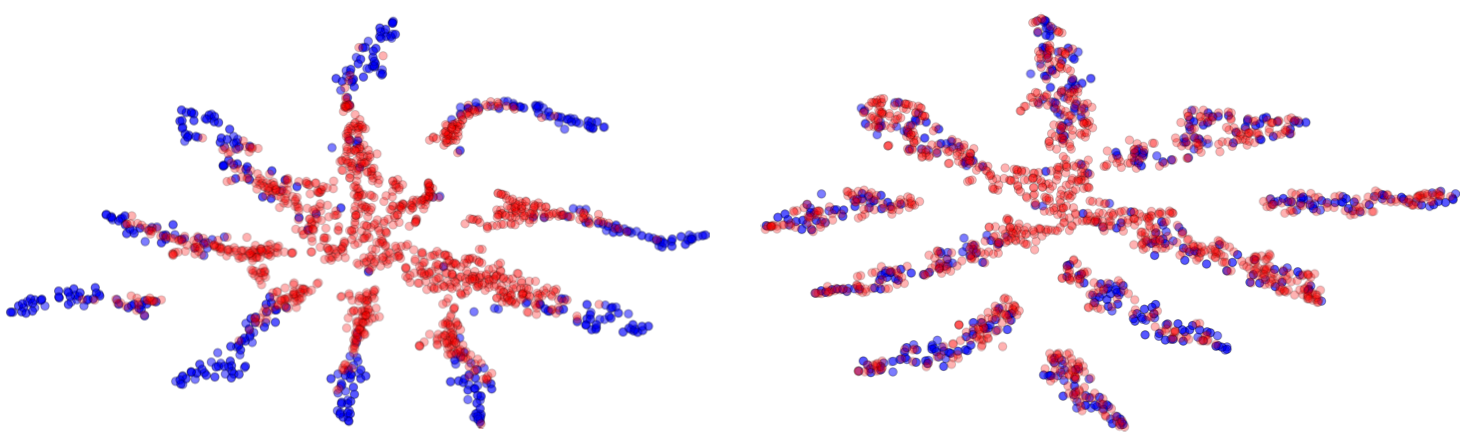
\includegraphics[width=0.8\textwidth]{assets/DomainAdaptation.png}
\caption[The Effect of Domain Adaptation]{\textbf{The effect of domain adaptation.} The blue (red) points represent samples from the source (target) domain. Each point represents the position of an element in a two-dimensional feature space. Shown are features from the last hidden layer of a DNN classifier. In the left plot no domain adaptation is performed. The source samples form separated groups while the target samples are more centered and less separated. In the right plot, the domain adaptation is used during the training. Source and target samples cover the same areas, the predictions of target samples are more reliable. Source: \cite{DA_Adversarial}}
\label{fig:ch_4_DomainAdaptation}
\end{figure}

\subsection{Moments Method}
Two distributions are the same if and only if the moments of these distributions are identical. The first moment of a distribution is the mean
\begin{equation}
\mu = E[X] = \frac{1}{n}\sum_{\{x \in X\}} x \quad ,
\end{equation}
where $x \in X$ are data points from the distribution $X$ and $n$ is the number of all data points. Central moments are defined as 
\begin{equation}
\mu^{(k)} = \frac{1}{n} \sum_{\{x \in X\}} E\left[\left(x-E[X]\right)^k\right] \quad ,
\end{equation}
where $(k)$ denotes the order of the moment. The second central moment is the variance. Higher central moments are normalized by the standard deviation to the power of $k$
\begin{equation}
\hat{\mu}^{(k)} = \frac{\mu^{(k)}}{\sigma^k} \quad .
\end{equation}

These moments can be used to measure the domain discrepancy in certain features. A simple measure is the maximum mean discrepancy (MMD) \cite{MME} 
\begin{equation}
\textrm{MMD}_i(X_\textrm{S},X_\textrm{T}) = \left|\mu_{i}(X_\textrm{S}) - \mu_{i}(X_\textrm{T}) \right| \quad ,
\end{equation}
where $i$ denotes the feature and $S$ ($T$) denotes the source (target) domain. The MMD is used in many domain adaptation approaches, for example \cite{DDE}. It can be used as an additional term in the loss function to construct a domain invariant feature space. The resulting loss function is given by
\begin{equation}
L = L_\textrm{C}(X_\textrm{S},y) + \lambda \sum_i \textrm{MMD}_i^2(X_\textrm{S},X_\textrm{T}) \quad ,
\end{equation}
where the $L_\textrm{C}(X_\textrm{S},y)$ is the classification loss with the labels $y$ of the samples from the source domain. The hyperparameter $\lambda$ determines how strong the domain discrepancy is punished. This approach is generic, one can use any features, for example the ones of some hidden layer or the output layer. The training is performed with samples from both domains at the same time while only samples from the source domain can be used for the training of the classification. \\

A better measure for the domain discrepancy includes higher central moments. The loss can be defined as 
\begin{equation}
L = L_\textrm{C}(X_\textrm{S},y) + \alpha \sum_i \textrm{MMD}_i^2(X_\textrm{S},X_\textrm{T}) + \beta \sum_i \left( \mu^{(2)}_{i}(X_\textrm{S}) - \mu^{(2)}_{i}(X_\textrm{T}) \right)^2 + \dots \quad ,
\end{equation}
with the hyperparameters $\alpha$ and $\beta$. The dots represent the possibility to include arbitrary higher moments. 


\subsection{Domain-Adversarial Method}
The domain-adversarial method (or domain adaptation by backpropagation) was introduced in \cite{DA_Backprop, DA_Adversarial}, the proposed architecture is shown in figure \ref{fig:ch_4_DA_Backprop}. The method is realized through an extension to the original feed-forward DNN. The original DNN is divided into two parts. The first part is the feature extractor $G_f(\cdot;\theta_f)$ which maps the input features to a latent feature vector $\vec{f}$ and forwards them to the second part. The second part is the label predictor $G_y(\cdot;\theta_y)$, which predicts the class labels $y$. The additional part is the domain classifier $G_d(\cdot;\theta_d)$, which is used to distinguish between the source domain and the target domain. As the label predictor, the domain classifier takes $\vec{f}$ as its input features. The first layer is a gradient reversal layer (GRL) followed by an arbitrary number of feed-forward layers and one binary output neuron. The GRL has no free trainable parameters, it is the identity function in forward propagation. During backpropagation, the gradient is multiplied by the negative constant $-\lambda$.\\ 

\begin{figure}
\centering
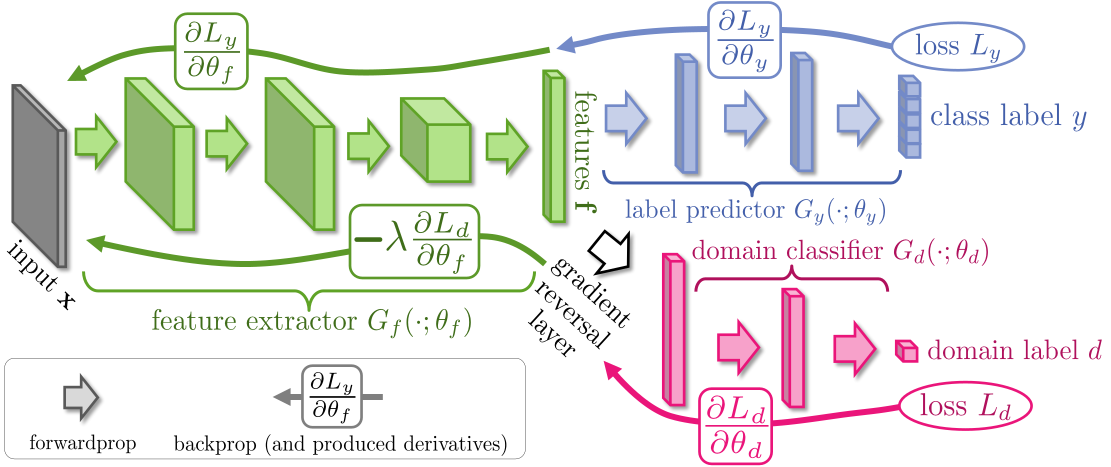
\includegraphics[width=0.9\textwidth]{assets/gradReversal.png}
\caption[Domain-Adversarial Method]{\textbf{The domain-adversarial method.} The input features $\vec{x}$, the feature extractor (green) and the label predictor (blue) form a conventional DNN. Additionally, a domain classifier (red) is added. For a more detailed description refer to the text. Source: \cite{DA_Adversarial}}
\label{fig:ch_4_DA_Backprop}
\end{figure}

During training, samples from the source domain and target domain are used at the same time. As a loss function for the label predictor, denoted as class loss $L_y$, the categorical cross entropy can be used. The class loss takes only the labeled samples from the source domain into account, backpropagation is used to update the free parameters $\theta_y$ of the label predictor and the free parameters $\theta_f$ of the feature extractor. For the domain classifier, a binary cross entropy can be used as a loss function, denoted as domain loss $L_d$. The domain loss includes samples from both domains. The free parameters $\theta_d$ of the domain classifier are updated by backpropagation in a way that the discrimination between the domains is improved. Through the gradient reversal layer, the gradient is flipped and the $\theta_f$ are updated towards a maximum of the domain loss. As a result $\vec{f}$ becomes indistinguishable between source and target domain, this is called $\vec{f}$ becomes domain invariant. This also leads to domain invariant class labels. The updated free parameters can be computed using a standard optimizer. For the SGD, they are given by
\begin{equation}\label{eq:ch_4_Backprop}
\begin{split}
\theta_f \quad &\leftarrow\quad  \theta_f - \eta \left( \frac{\partial L_y}{\partial \theta_{f}} - \lambda \frac{\partial L_d}{\partial \theta_{f}} \right) \quad ,\\
\theta_y \quad &\leftarrow\quad  \theta_y - \eta \left( \frac{\partial L_y}{\partial \theta_{y}} \right)\quad ,\\
\theta_d \quad &\leftarrow\quad  \theta_d - \eta \left( \frac{\partial L_d}{\partial \theta_{d}} \right) \quad .
\end{split}
\end{equation}
Note that this is done implicitly through the use of the GRL, no further changes have to be done to the optimizer. The first and third equation in \ref{eq:ch_4_Backprop} show that $\theta_d$ minimizes the domain loss while $\theta_f$ maximizes it, the factor $\lambda$ is a trade-off factor between these two mechanisms. The domain classifier can therefore also be seen as an adversarial network, similar to the general adversarial network (GAN) approach of \cite{Goodfellow}. 



%FIXME GRL im anhang

%FIXME
%\section{A Figure of Merit: The Kolmogorov-Smirnov-Test}


\chapter{Heavy Flavor Jet Tagging}
Jets that origin from the heavy flavor quarks c and b have characteristic properties compared to jets that origin from gluons or light flavor quarks, which are u, d, and s quarks. The properties are essentially determined through the bound state hadrons formed by the quarks and are explained in section \ref{sec:ch_tag_properties}. These properties can be used to distinguish the jets in respect of present quark flavors (tagging). This is done using a fully connected feed-forward MLP in the DeepCSV algorithm, which is explained in section \ref{sec:ch_deepCSV}. A more advanced DNN is used by the DeepFlavour algorithm that is described in \ref{sec:ch_deepFlavour}.

\section{Heavy Flavor Jet Properties}\label{sec:ch_tag_properties}
\begin{figure}
\centering
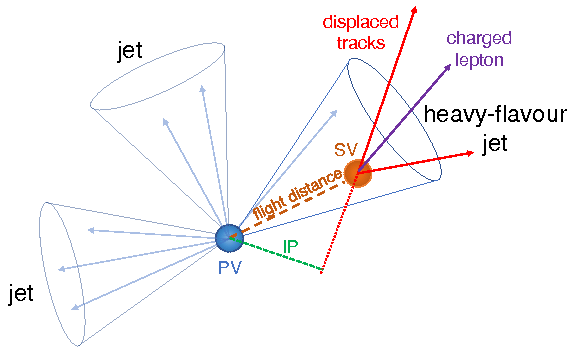
\includegraphics[width=0.6\textwidth]{assets/SV.png}
\caption[Heavy Flavor Jet]{\textbf{A heavy flavor jet.} Several jet properties can be used to identify a heavy flavor jet. The main identifying properties are secondary vertices (SV) and displaced tracks with an impact parameter (IP) towards the primary vertex (PV).  Source: \cite{HeavyFlavorIdentification}}
\label{fig:ch_5_SV}
\end{figure}

B (C) hadrons have a lifetime in the order of 1.5\,ps (1\,ps) \cite{HeavyFlavorIdentification}, depending on their momentum, this results in a flight distance of some mm up to cm in the CMS detector. After this distance they decay at a secondary vertex (SV) where daughter particles arise. The SVs itself have characteristic properties, for example the vertex mass, which is the invariant mass of the SV. Another important variable is the flight distance (FD), defined as the distance from the PV to the SV. The FD can be measured in three spatial dimensions (3D), in the plane transverse to the beam line (2D) or in one dimension along the beam line (longitudinal). The tracks of the daughter particles can be propagated towards the beam line. The distance of their closest approach to the primary vertex is called impact parameter (IP). The daughter particles tend to have larger IPs compared to tacks that origin from the PV, they have displaced tracks. These aspects are outlined in figure \ref{fig:ch_5_SV}. The IP can be measured similar to the FD in 3D, 2D or in longitudinal direction. The higher mass of the B or C hadrons compared to hadrons consisting of only light flavor quarks results in daughter particles with higher momentum perpendicular to the jet axis. Furthermore, b or c quark decays mostly happen through flavor-changing charged currents under the emission of a W boson, which in turn can decay into an electron or a muon. Therefore, b (c) jets contain an electron or a muon in about 20 \% (10 \%) \cite{HeavyFlavorIdentification} of the cases. Since b quarks decay mostly first in c and than in light quarks (see equation \ref{eq:ch_1_V}), they have in general several SVs and a higher probability of containing electrons or muons. 

\subsection{Secondary Vertex Reconstruction}
The reconstruction of the SV is done with the inclusive vertex finding (IVF) algorithm \cite{IVF}. The IVF algorithm takes all tracks with $\pt > 0.8\, \GeV$ and longitudinal IP $< 0.3\, $cm into account. In a first step, seed tracks with thresholds on the IP and the IP significance (the IP value divided by its significance) are identified. Next, tracks are clustered if they form a compatible SV. The clustered set of tracks is then used to fit a SV. Afterwards, SVs are only kept if their 2D FD significance (the FD value divided by its significance) is larger than 2.5 and their 3D FD significance is larger than 0.5 and no other SV is compatible with the tracks. Furthermore are tracks removed if $\Delta R$ between the track and the SV flight direction is larger than 0.4. After this cleaning, a repeated SV fitting is performed followed by a repeated cleaning. The remaining SVs have a FD significance (the FD value divided by its significance) of 10 or more and less than 20\ \% of their tracks shared with other SVs.\\

%\section{CSVv2 Algorithm}



\section{The DeepCSV Algorithm}\label{sec:ch_deepCSV}
The DeepCSV algorithm used in this thesis consists of a DNN with five hidden layers with 100 neurons each. The DNN uses up to 66 input features to get a good separation of the jets in four different categories. This results in 66 neurons in the input layer and 4 neurons in the output layer. The implementation is done using the high-level API Keras \cite{Keras} with the machine learning framework TensorFlow \cite{Tensorflow} as back end.\\

For the hidden layers, ReLu activation functions are used while the last layer has softmax activation functions. The loss function is the categorical cross-entropy. After each hidden layer, a dropout layer with a dropout rate of 0.1 is used (see section \ref{sec:ch_4_perceptron} and \ref{sec:ch_4_mlp}). 

\subsection{Categories}
In this thesis, jets were distinguished in four categories, which are b, bb, c and udsg. Jets containing two B hadrons are categorized as bb. Jets containing one B hadron are categorized as b. Jets in which no B hadron is present, but at least one C hadron, are categorized as c. If neither a B hadron nor a C hadron exists, the jet is categorized as udsg. Jets that origin from pileup remain uncategorized. The simulated jets are labeled corresponding to their categories in the 1-of-K coding scheme (as in section \ref{sec:ch_4_training}). \\

\subsection{Input Features}
The DeepCSV algorithm makes use of the properties described in section \ref{sec:ch_tag_properties}. It takes into account global jet properties with twelve features, six charged particle tracks with seven features each, four neutral particle tracks with one feature each and one secondary vertex with eight features. The particle tracks from PF elements and the reconstructed SVs are first selected by demanding some quality criteria. Afterwards, the six most displaced charged tracks and the four most displaced SVs are taken. For the neutral particles, the ones with the highest \pt are selected. The used variables and their description are found in \cite{HeavyFlavorIdentification}.\\

%\begin{description}
%\setlength{\itemsep}{-20pt}
%\item[$\pt(j)$:] Jet \pt\\
%\item[$\eta(j)$:]  Jet $\eta$\\
%\item[$N_\textrm{SV}$:] Number of secondary vertices in the Jet\\
%\item[${E_\textrm{T}(\sum tracks)}$/${E_\textrm{T}(j)}$:] The transverse energy of the sum of the four-momentum vectors of the selected tracks divided by the transverse energy of the jet. \\
%\item[$\Delta R(\sum tracks, j)$:] $\Delta R$ between the sum of all four momentum vectors of the selected tracks and the jet axis\\
%\item[Vertex category:] One of three categories, (1) a SV is present. (2) there are tracks that are consistent with a SV under looser criteria. (3) none of the previous cases occur.\\
%\item[first track $\sigma_{n\textrm{2D,IP}}$ above c] The $\sigma_{n\textrm{2D,IP}}$ of the first track that raises the invariant mass above $1.5\,$\GeV when sequentially summing up the four momenta of all tracks.
%\end{description}

During the training, the convergence of the DNN is faster if all input features have the same mean and variance. Therefore, each input feature $i$ is rescaled by using its mean value $\mu_i$ and standard deviation $\sigma_{i}$. The normalized input values $\hat{x}_i$ are then given by
\begin{equation}
\hat{x}_i = \frac{x_i - \mu_i}{\sigma_{x,i}} \quad ,
\end{equation}
and have a mean value of 0 and a standard deviation of 1. If a feature is missing for a certain jet, a default value is assigned that is not overlapping with the core of the feature distribution and close to zero. 

%\subsection{Training}
%The DeepCSV algorithm is trained on jets from \ttbar events and QCD events

\section{The DeepFlavour Algorithm}\label{sec:ch_deepFlavour}
The DeepFlavour algorithm \cite{DeepFlavour} is a further development of the DeepCSV algorithm. In contrast to the DeepCSV algorithm, the selection of the tracks and vertices are much looser and much more candidates with more features of each PF candidate are included. Moreover the number of PF candidates varies for each jet. This requires an alternative flexible network structure that compresses the high amount of information. More information of jet tagging with advanced machine learning tools can be found in \cite{JetClassificationDNN}. 

\begin{figure}
\centering
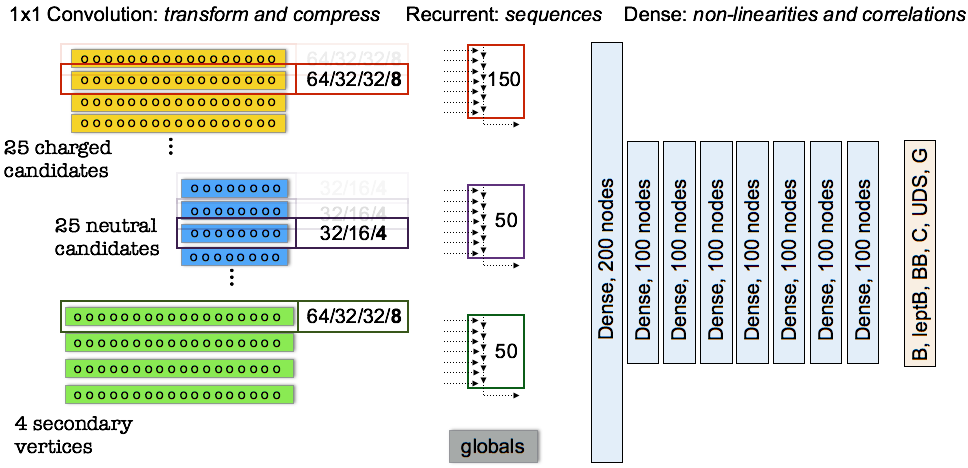
\includegraphics[width=0.8\textwidth]{assets/DF.png}
\caption[Architecture of the DeepFlavour Algorithm]{\textbf{Architecture of the DeepFlavour algorithm.} Charged particle tracks, neutral particle tracks, SVs and global jet information are inserted separately in the network and compressed through $1x1$ convolutional layers. The subsequent use of recurrent sequences leads to a more flexible structure in respect of the number of objects that are present in the jet. Together with the global features, the correlations between the object can be extracted. Source: With kind permission of Jan Kieseler}
\label{fig:ch_5_DF}
\end{figure}

\subsection{Architecture}
The network structure of the DeepFlavour algorithm is shown in figure \ref{fig:ch_5_DF}. The features are divided in four groups, namely the charged candidates, the neutral candidates, the secondary vertices and the globals. The first three groups consist of several objects of which each object has the same features. Therefore, each group is arranged separately as a two dimensional feature layer. The first dimension represents the different features while the second dimension represents the various objects. A maximum of 25 charged particles, 25 neutral particles and 4 secondary vertices is given, but there is no issue for jets with less objects. The two dimensional layer is inserted into a $1x1$ convolutional layer. This kind of layer is only fully connected in the first dimension and uses shared weights in the second dimension. The $1x1$ refers to the so called filter kernel size and if a bigger filter kernel size is used, the layer performs a convolution of the input features with the so called filter, hence the name convolutional layer. A $1x1$ convolutional layer is shown in figure \ref{fig:ch_5_Conv}.\\

\begin{figure}
\centering
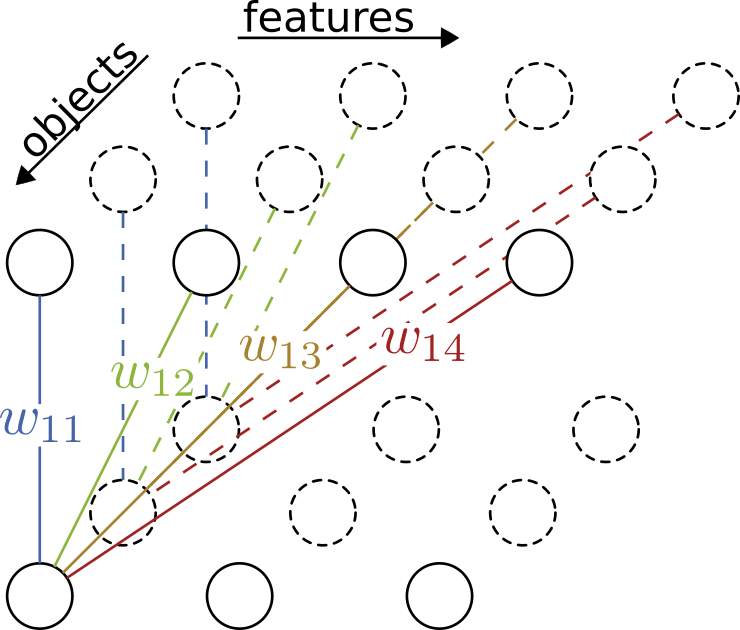
\includegraphics[width=5cm]{assets/convolutional.png}
\caption[$1x1$ Convolutional Layer and LSTM Unit]{\textbf{$1x1$ convolutional layer.} Shown are three objects with four features each. The objects share their weights among themselves, the lines in the same color represent the same weights. For each filter, one output neuron is generated for each object. In this case, three filters were used.}
\label{fig:ch_5_Conv}
\end{figure}

The $1x1$ convolutional layer generates output features which are again two-dimensional. In the first dimension, new latent features are constructed while the second dimension represents the same objects as before. For the charged particles and SVs, four $1x1$ convolutional layers are connected in a row, they use 64, 32, 32 and 8 filters respectively. The neutral particles are processed in three $1x1$ convolutional layers with 32, 16 and 4 filters each. Each two-dimensional output of the last $1x1$ convolutional layer is then inserted into a long short-term memory (LSTM) \cite{LSTM} layer. The LSTM layer takes sequences of features as input, in this case the sequences are the various objects.\\

\begin{figure}
\centering
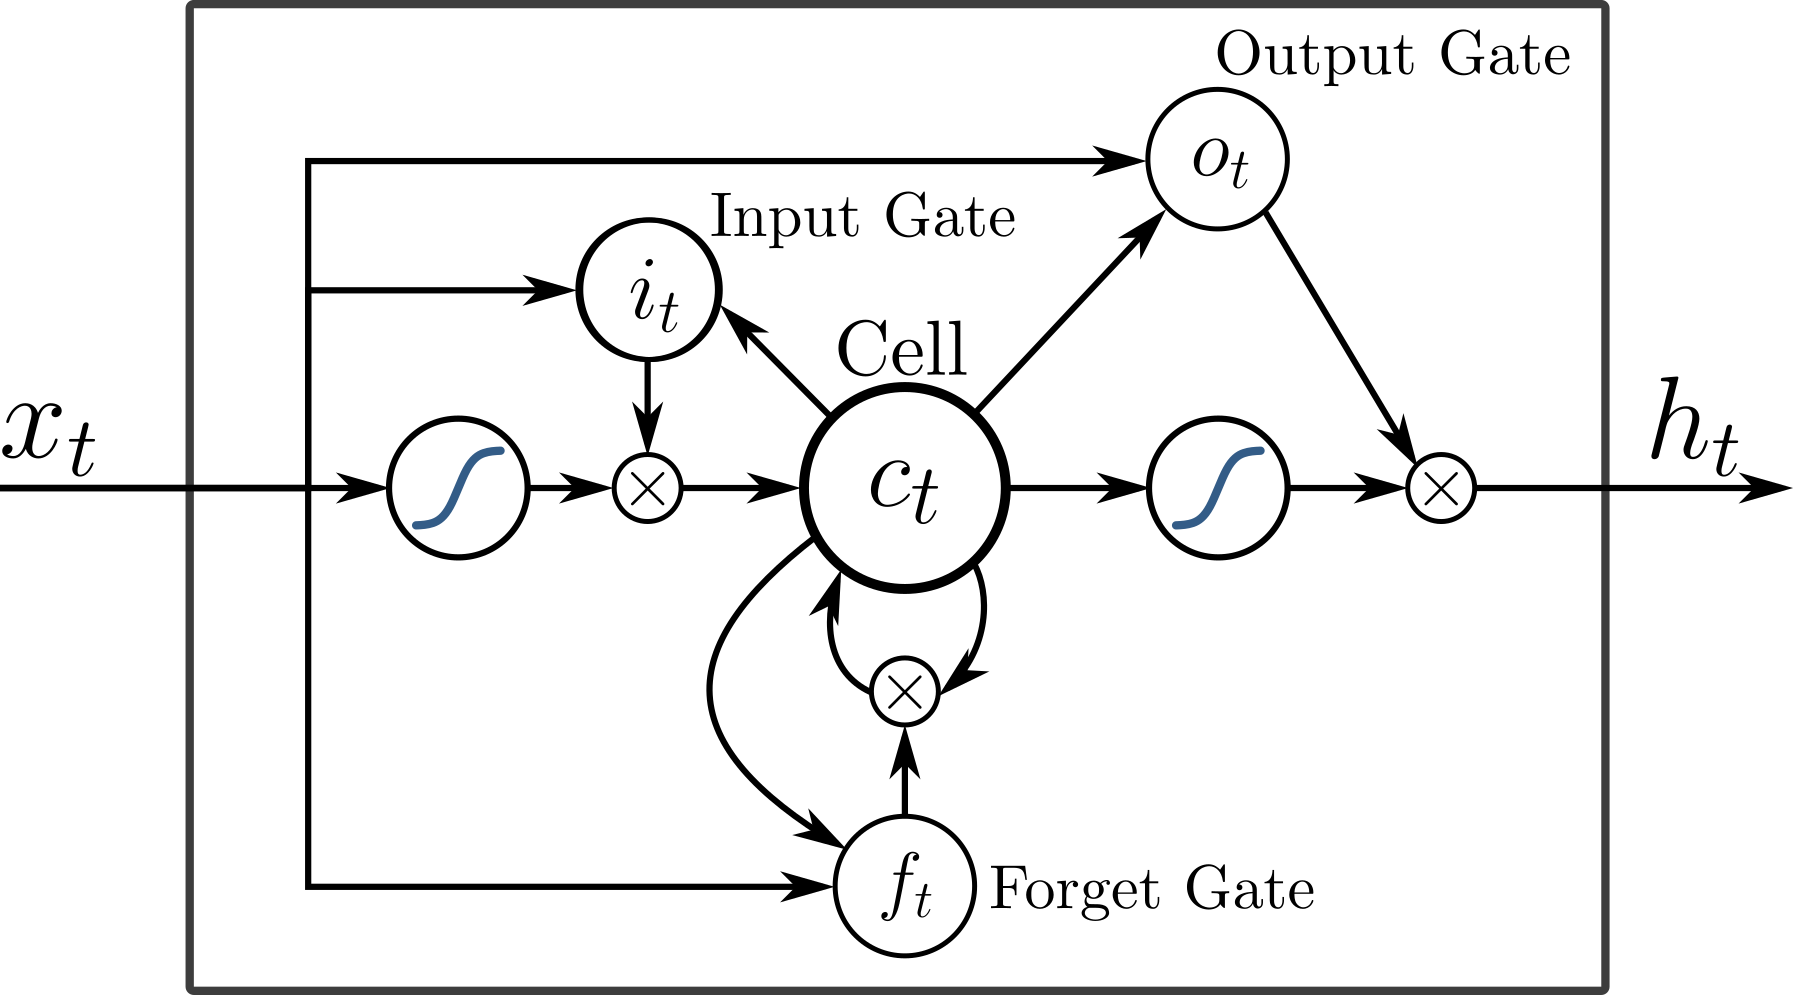
\includegraphics[width=7cm]{assets/lstm.png}
\caption[Long Short-Term Memory Unit]{\textbf{Long short-term memory (LSTM) unit.} The LSTM unit transports the input vector $x_t$ to three gates. The input gate $i_t$ determines how much a new value influences the memory cell $c_t$, the forget gate $f_t$ describes the degree the value of $c_t$ is forgotten and the output gate defines the impact of $c_t$ in the output. Adapted from \cite{LSTMunit}.}
\label{fig:ch_5_LSTM}
\end{figure}

Each unit of the LSTM layer has a memory and is therefore capable of taking past sequences into account. One LSTM unit is shown in figure \ref{fig:ch_5_LSTM}. The most information can be extracted from the last sequence, therefore the sequences have to be ordered in a way that the most important sequence is inserted as the last sequence. The output of the LSTM layer is one dimensional and can be chosen freely. For the DeepFlavour algorithm, 150 units were taken for the charged particles and 50 each for the neutral particles and SVs. The outputs of the three LSTM layers from the three categories respectively are concatenated together with the features of the globals into one flat layer. These are connected to a fully connected layer with 200 neurons and followed by seven fully connected layers of 100 neurons each.\\

The LSTM layer uses hyperbolic tangent activation functions. For the other hidden layers, ReLu activation functions were used. The output layer has again sigmoid activation function. The loss function is again the categorical cross-entropy and dropout layers are applied after each hidden layer with a dropout rate of 0.1. Additionally, a batch normalization layer is applied after each hidden layer (see section \ref{sec:ch_4_perceptron} and \ref{sec:ch_4_mlp}). 


\subsection{Categories}
The categories are similar to the ones used in the DeepCSV algorithm with the difference that the DeepFlavour algorithm distinguishes between the light quarks u,d and s and gluons g, where the physics definition is used as explained in \cite{MCTruth}. Moreover it differentiates between B hadron jets where the B hadron decays leptonically or hadronically. The labeling is done in the same way as in the DeepCSV algorithm.

\subsection{Input Features}
Compared to the DeepCSV algorithm, the set of input features has been increased. 15 global features, 16 features for each charged particle, 6 features for each neutral particle and 12 features for each SV were used. For the sequential processing of the LSTM layers, the objects have to be ordered. Charged particles and SVs are sorted in respect of the 2D IP significance in descending order. Charged candidates that were used in the PV fit do not have a 2D IP significance, they are sorted in ascending order of the $\Delta R_m(cPF,SV)$ value ($\Delta R$ of the charged candidate and its closest SV in the jet). For jets without SV, the particle \pt is used in descending order as a third criterion. Neutral PF candidates are sorted as a first criterion in ascending order by their $\Delta R_m(nPF,SV)$ value and as a second criteria descending by their {\pt}.

\section{Performance of b Tagging Algorithms}
To measure the performance of a tagging algorithm, the so called receiver operating characteristic (ROC) curve can be used. The ROC curve is computed by varying the test statistic (section \ref{sec:ch_4_classification}) of the classifier output from its minimal to its maximal value. At each point the efficiency and the FPR are calculated. The ROC curve is commonly computed on simulated samples with the available labels. The performances of the DeepCSV and DeepFlavour algorithms are compared to the CSVv2 algorithm which is a well established b tagging algorithm in the CMS experiment. Their ROC curves are shown in figure \ref{fig:ch_5_Performance}. The classifier is applied at a fixed value of the test statistic, the so called working point. The working point is defined by the FPR. The loose working point (L) has a FPR of 1 \%, the medium working point (M) has a FPR of 0.1 \% and the tight working point (T) has a FPR of 0.01 \%. \\

\begin{figure}
\centering
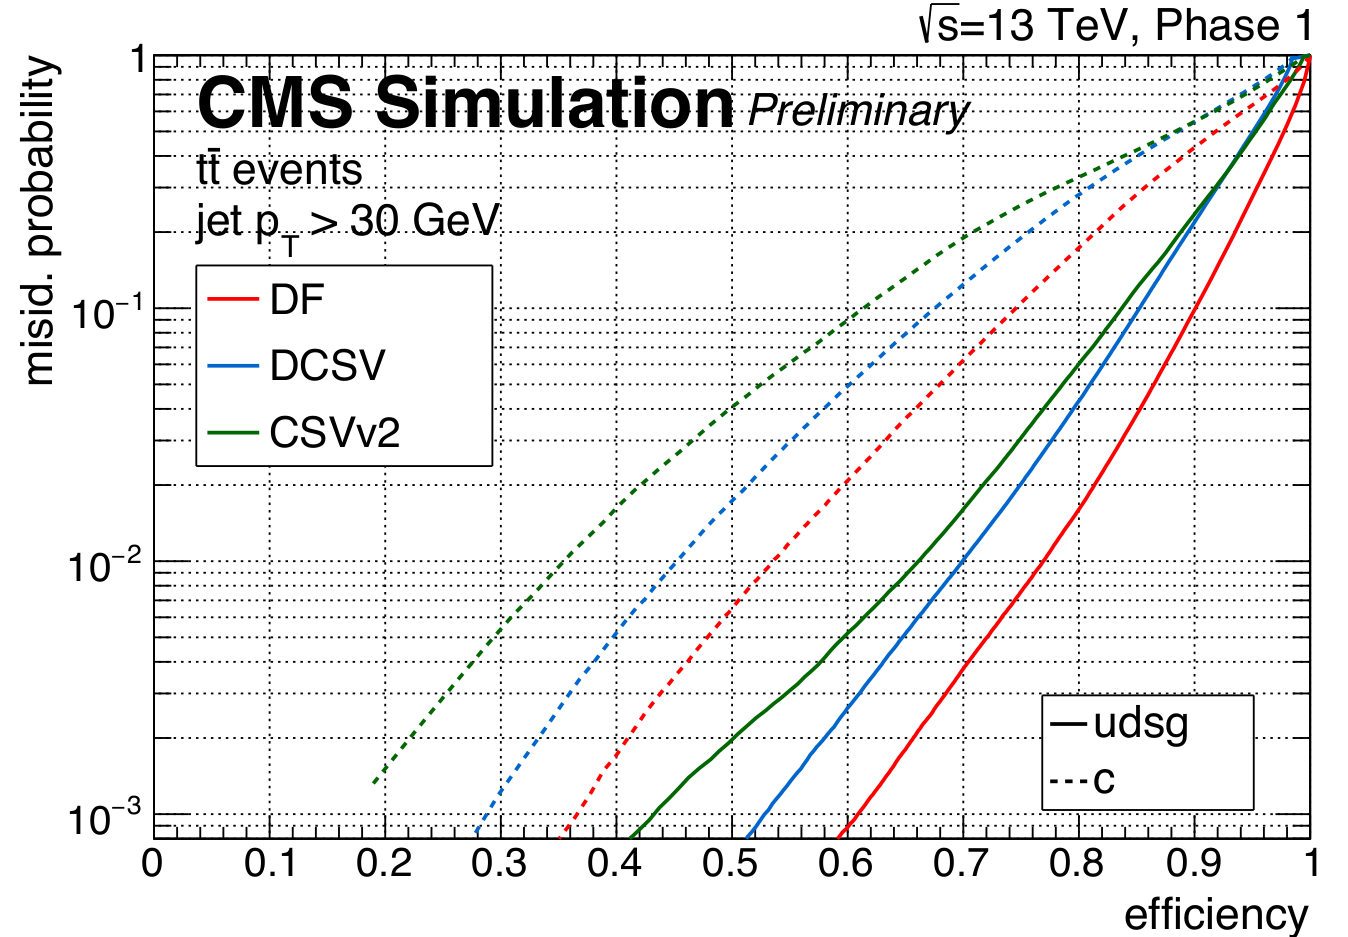
\includegraphics[width=10cm]{assets/performance.png}
\caption[Architecture of the DeepFlavour Algorithm]{\textbf{Performance of b tagging algorithms.} The plot shows the misidentification probability (which is the FPR) against the b tagging efficiency measured on simulated samples. The b tagging efficiencies against light quarks and gluons (continuous lines) and c quarks (dashed lines) are shown for three different tagging algorithms. The CSVv2 algorithm has the worst performance. The DeepCSV (DCSV) is the currently proposed b tagging algorithm for CMS analyses. The DeepFlavour (DF) has the best performance, it is under development and the performance on real data is currently not known. Source: \cite{DeepFlavour}}
\label{fig:ch_5_Performance}
\end{figure}
%TODO figure not in reference! 

To calculate the efficiency in data, more complex methods have to be applied. Since these methods have model assumptions and the number of jets from data events is much more limited, they have high systematic and statistical uncertainties. With the efficiency on data $\epsilon_\textrm{data}$ and on simulated jets $\epsilon_\textrm{MC}$ on identical FPRs, a scalefactor can be computed as
\begin{equation}
SF_b = \frac{\epsilon_\textrm{data}}{\epsilon_\textrm{MC}} \quad .
\end{equation}
Scalefactors for the DeepCSV and CSVv2 algorithm computed with various methods are shown in figure \ref{fig:ch_5_Scalefactor}. As expected, the scalefactor is in the most cases lower than one, this origins from the fact that the algorithms are trained on simulation and have therefore worse performance on data. More important than a scalefactor that is close to one is a scalefactor with low uncertainty. However, scalefactors which are far from one tend to have higher uncertainties. For the DeepFlavour algorithm, there exists no official measurement of the scalefactors, but scalefactors with higher uncertainties are expected since the unselected tracks and vertices, used by the DeepFlavour algorithm are less good modeled compared to the ones used by the DeepCSV algorithm.

\begin{figure}
\centering
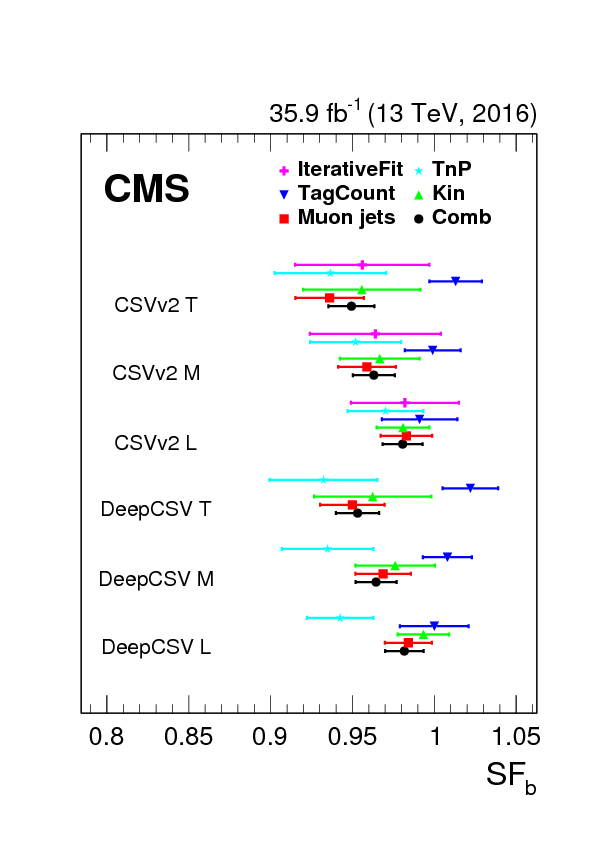
\includegraphics[width=6cm]{assets/SF.png}
\caption[Scalefactors for b Tagging Algorithms]{\textbf{Scalefactor for b tagging algorithms.} The scalefactor for the b tagging algorithms at different working points are shown for five methods. The measured scalefactors agree in their uncertainties. The black dot refers to the combined value and is mainly dominated by the Muon Jets method. Source: \cite{HeavyFlavorIdentification}}
\label{fig:ch_5_Scalefactor}
\end{figure}

\chapter{Event Selection}

The subject of this thesis is to study the effect of domain adaptation methods on flavor tagging algorithms to improve the data to simulation agreement. In section \ref{sec:ch_4_da} two domain adaptation methods were introduced. Both have the goal to transfer the source domain and the target domain into a domain invariant feature space that the classifier output becomes domain invariant. To achieve this goals, the source and the target distribution of their input features have to be similar. Furthermore, both domains should have the same distributions in their class compositions. Which means in this case they need to have the same amount of jets each quark flavor in data and simulation. In order to meet these requirements, an event selection is needed. \\

The event selection has several requirements to fulfill. It has to be performed in the same way for data and simulation and the data to simulation agreement for the selected events shall be as good as possible. The mismodeling of the simulation of the jets shall be the dominant reason for the domain discrepancy. The event selection has to be independent of the specific jets in each event. Moreover the selected events should contain balanced fractions of jets of the different categories used in the classifier. Finally the amount of jets should be high enough that the statistical uncertainties are negligible. The last two points are in direct conflict as categories like bb occur mostly for high \pt jets of which not many exist. Therefore the demand of balanced fractions is secondary. 

\section{Top Quark Decay}

\begin{figure}
\hfill
\subfigure[]{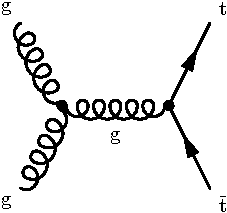
\includegraphics[width=3cm]{assets/Feynman/tt_gg_s.pdf}}
\hfill
\subfigure[]{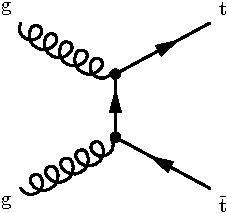
\includegraphics[width=3cm]{assets/Feynman/tt_gg_t.pdf}}
\hfill
\subfigure[]{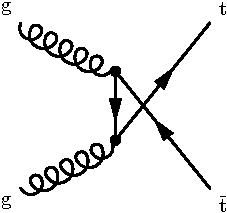
\includegraphics[width=3cm]{assets/Feynman/tt_gg_u.pdf}}
\hfill
\subfigure[]{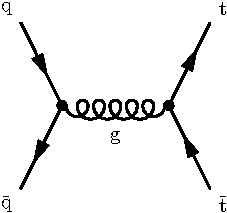
\includegraphics[width=3cm]{assets/Feynman/tt_qq_s.pdf}}
\hfill
\caption[Dominant Processes of Top Quark Pair Production]{\textbf{Dominant processes of top quark pair production at the LHC.} Top quark pair production by gluon fusion is the dominant process at the LHC. It occur in the s channel (a), in the t channel (b) and in the u channel (c). Another production process of the same order of perturbation theory is the quark-antiquark annihilation in the s channel (d). Because of the PDFs, this channel is less contributions.}
\label{fig:ch_5_ttProduction}
\end{figure}

A good choice is to search for top quarks as they decay almost every time into a b quark and a W boson. Moreover, the t$\bar{\textrm{t}}$ process is under investigation by many analyses, these can be taken into comparison (for example \ref{ttbarSemilep, ttbarDilep}). The W boson decays either into a lepton and a neutrino, or into a quark-antiquark pair. Top quarks are mainly produced in pairs at the LHC with a cross section of $\sigma_{\textrm{t}\bar{\textrm{t}}} = 831\, $pb at $\sqrt{s} = 13\,\TeV$ (predicted by the SM \cite{TopPPw}). Their decay can be categorized by the decay of the W bosons as the potential lepton is a good indicator for those events. If both W bosons decay into quarks, it is called a hadronic decay. If both W bosons decay into leptons, it is called a dileptonic decay. If one W decays into a lepton while the other into quarks, it is called semileptonic decay. The decay rates for the W boson and t$\bar{\textrm{t}}$ pairs are listed in table \ref{tab:ch_6_DecayRates}. The leading Feynman diagrams for top quark pair production are shown in figure \ref{fig:ch_5_ttProduction}. \\

\begin{table}[t]
\caption[Decay Modes of W Bosons and Top Quark Pairs]{\textbf{Decay modes of W bosons and top quark pairs.} Shown are the measured branching ratios from \cite{pdb}. In almost 50 \% of the cases of a hadronic W decay, a c quark occurs, the $X$ denotes a d or s quark. The $\uptau$ lepton often decays into quarks and is therefore often seen as a hadronic decay mode. In this table, the $\uptau$ is included as a lepton $\ell$.}
\label{tab:ch_6_DecayRates}
\begin{tabular}{llS[
                 table-number-alignment = center,
                 separate-uncertainty = true,
                 table-figures-uncertainty = 2,
                 table-figures-decimal = 2
         ]}
\toprule
{Particle} & {Decay mode} & {Branching ratio in \%} \\ 
\midrule
$\textrm{W}^+$ & $\textrm{e}^+\ +\ \bar{\upnu}_\textrm{e}$ & 10.71 \pm 0.16\\
$\textrm{W}^+$ & $\upmu^+\ +\ \bar{\upnu}_\upmu$ & 10.63 \pm 0.15\\
$\textrm{W}^+$ & $\uptau^+\ +\ \bar{\upnu}_\uptau$ &  11.38 \pm 0.21\\
$\textrm{W}^+$ & q + $\bar{\textrm{q}}$ & 67.41 \pm 0.27\\
$\textrm{W}^+$ & c + $X$ & 33.3 \pm 2.6\\
t$\bar{\textrm{t}}$ & hadronic (all-jets) & 45.7\\
t$\bar{\textrm{t}}$ & semileptonic ($\ell$ + jets) & 43.8\\
t$\bar{\textrm{t}}$ & dileptonic ($\ell\ell$) & 10.5\\
\bottomrule
\end{tabular}
\end{table}

The t$\bar{\textrm{t}}$ hadronic decay mode has the best statistic but is inappropriate for a selection as only jets are in the final states and other effects have the same signature and occur far more often. The t$\bar{\textrm{t}}$ semileptonic decay mode has also a high statistic and with the lepton in the final state, a good indicator for this process exists. As listed in table \ref{tab:ch_6_DecayRates}, t$\bar{\textrm{t}}$ semileptonic decays also provide some c quarks. Therefore, selection criteria are applied in respect of the t$\bar{\textrm{t}}$ semileptonic decay mode. This is described in section \ref{sec:ch_6_semilep}. A much lower statistic has the t$\bar{\textrm{t}}$ dileptonic decay mode. But events of this category that decay into a electron muon pair with opposite flavor and charge produce the clearest signal. In section \ref{sec:ch_6_dilep} this selection is described.

\section{Particle Identification}
The $\tau$ decays before it can be directly identified, therefore it is less suited for a selection. The main identifying objects are electrons and muons. In a first selection step, quality criteria are applied on these particles and an isolation is required. The set or remaining muons and lepton candidates have a low fake rate and can be used for the decay mode selection. 
Moreover, jets have a high fake rate as for example photons are often misidentified as jets. This requires a further selection. 

\subsection{Muon Selection}
Muon-quality requirements are used in many analyses, several requirements are combined in so called muon IDs. In this thesis the muon is required to fulfill the tight muon ID. The tight muon ID contains requirements of the number of hits of the muon track in various detector components or a minimum value of $\chi^2$ divided by the number of decreases of freedom of the fit. Apart from this, in this thesis muons with $|\eta| < 2.4$ are discarded as these are not fully covered from the muon chamber. A minimum \pt value is required as the modeling of low \pt muons is worse, the \pt cut has a different value in each selection.  Additionally an isolation criteria of $I_l^{\textrm{PF}/\Delta \upbeta} < 0.15$ is applied as described in section \ref{sec:ch_3:Isolation}. The set of selected muons is denoted as good muons.

\subsection{Electron Selection}
For the electrons, a similar ID, the tight electron ID is applied. Furthermore, to ensures the best performance of the silicon tracker the electron is required to have a value of $|\eta| < 2.4$. However there is a gap in the ECAL between the barrel and the endcap part, therefore electrons in the interval of $1.4442 < |\eta_\textrm{SC}| < 1.5660$ are excluded, where $\eta_\textrm{SC}$ refers to the position of the ECAL supercluster of the electron. Additionally, cuts on the IP have to b e performed to reduce pileup contributions. The transverse IP has to be lower than 0.05 (0.1) while the longitudinal IP has to be lower than 0.1 (0.2) for electrons with $|\eta_\textrm{SC}| < 1.4442$ ($|\eta_\textrm{SC}| > 1.5660$). Furthermore a $\pt > 20\,\GeV$ is required due to the mismodeling of low \pt electrons. The set of selected electrons is denoted as good electrons.

\subsection{Jet Selection}
The Jet selection is performed by requiring
\begin{description}
\setlength{\itemsep}{-20pt}
\item[•] \pt > 30 as those jets have a low probability to come from the hard scattering process,\\
\item[•] $|\eta| < 2.4$ to ensure the full capability of the detector,\\
\item[•] neutral electromagnetic energy fraction < 0.99 to exclude photons modeled as jets,\\
\item[•] charged electromagnetic energy fraction < 0.99 to exclude electrons modeled as jets,\\
\item[•] neutral hadron energy fraction < 0.99 to exclude single neutral hadrons modeled as jets,\\
\item[•] charged hadron energy fraction > 0 as a jet should have charged hadrons,\\
\item[•] number of charged and neutral candidates > 1 to exclude single particles reconstructed as jets,\\
\item[•] and number of charged candidates > 0 as a jet should have charged particles.
\end{description}
Finally, jets are rejected if a good electrons or a good muons has a closer distance than $\Delta R = 0.4$. The set of selected jets is denoted as good jets.

\section{Top Quark Pair - Semileptonic Selection} \label{sec:ch_6_semilep}
The final state particles of a t$\bar{\textrm{t}}$ semileptonic decay in LO in QCD are one lepton, one neutrino, two b quarks, one up-type and one down-type quark. The best signal is obtained in the case where the lepton is a muon, the selection criteria are
\begin{description}
\setlength{\itemsep}{-20pt}
\item[•] one good muon with \pt > 30,\\
\item[•] no additional good muon or good electron,\\
\item[•] four good jets with no further requirements on the jets,\\
\item[•] a transverse mass of the W boson $m_{\textrm{T,W}} > 50\,\GeV$ to take the neutrino into account,\\
\item[•] a trigger selection, this will be explained later in this section.
\end{description}
A t$\bar{\textrm{t}}$ semileptonic decay mode that satisfies this selection is shown in figure \ref{fig:ch_6_semilep_mu}. The main contributions from other processes are from W boson production in association with jets and Drell-Yan processes ($qq \rightarrow X \rightarrow \ell\ell$ where $X$ is a photon or Z boson) in association with jets where one of the leptons misses the detector. A minor contribution is coming from single top quark production in association with jets. 

\begin{figure}
\centering
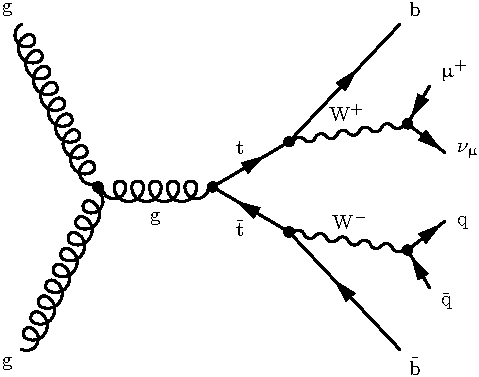
\includegraphics[width=0.4\textwidth]{assets/Feynman/semilep_mu_tt.pdf}
\caption[Semileptonic Decay of a Top Quark Pair]{\textbf{Semileptonic decay of a top quark pair.} The process is in LO of QCD in respect of the final state particles. To be unbiased of the selected jets, no selection for b jets is done. The quarks from the W boson decay are preferably light flavor or c quarks. The charged conjugated process is also possible.}
\label{fig:ch_6_semilep_mu}
\end{figure}

\subsection{Datasets}
The datasets for recorded events are sorted in respect of L1 triggers and the HLTs. The appropriate dataset for this selection is the single muon dataset. Each event was accepted by one or several HLTs of this category. For later steps, events are only taken if they passed one of two specific HLTs for isolated muons with $\pt > 24\GeV$. The use of a HLT selection on data and simulation ensures that no events from other datasets for data are represented in the simulated datasets. For the data, the recorded events from all periods of 2016 were taken. The total recorded luminosity is $\mathcal{L} = 35.14\,\textrm{fb}^{-1}$, it was computed using the \brilcalc \cite{brilcalc} tool.\\

The simulated events are sorted by the hard scattering process, additional jets can occur from pileup, initial or final state radiation or from the parton shower. The t$\bar{\textrm{t}}$ processes were generated by \powheg including NLO processes in QCD. For the W boson processes with additional jets, a dataset with NLO in QCD exists, this dataset is modeled with \amcatnlo and has negative lhe weights and the statistic is low. Alternative datasets exist in LO with more events. These are grouped in the number of jets in the final state of the hard process. The datasets for a W boson with two, three and four additional jets were taken. The Drell-Yan processes are generated with \amcatnlo and grouped in respect of the invariant mass $M_\textrm{inv}$ of the virtual photon or Z boson. Two datasets, one for $10\,\GeV < M_\textrm{inv} < 50\,\GeV$ and one for $M_\textrm{inv}>\,50\GeV$ were taken. The single t processes are grouped in respect of their production mode and generated with {\powheg}. The four main contributing production channels were taken, these are single top quark production in the t-channel and in association with an W boson and the corresponding processes for antitop quarks. The subsequent effects of all processes were modeled by \pythia 8 while the detector simulation is performed with {\geant}. The number of events and the cross section of each process are listed in table \ref{tab:ch_6_Datasets}.

\begin{table}[t]
\caption[Hard-Scattering Processes]{\textbf{Generated hard-scattering processes and their cross sections.} The higher the cross section $\sigma$ and the lower the number of generated events $N_{\textrm{gen}}$ is, the worse the statistic. One can see, the W + jets dataset has the worst statistic, in the semileptonic selection, it was chosen to take the jet grouped datasets instead. The processes where two bosons are involved have only a significant contribution in the dileptonic selection.}
\label{tab:ch_6_Datasets}
\begin{tabular}{lS[table-number-alignment = right]
					S[table-number-alignment = center,table-figures-decimal = 2]}
\toprule
{Dataset $\qquad$} & {$\qquad N_{\textrm{gen}}\qquad$} & {$\qquad\sigma$ in pb $\quad$} \\ 
\midrule
t$\bar{\textrm{t}}$ & 154948894 & 831.76 \cite{TopPP}\\
DY($10\,\GeV < M_\textrm{inv} < 50\,\GeV$) & 47946519 & 6025.2 \cite{DYCrossSec}\\
DY($M_\textrm{inv} > 50\,\GeV$) & 81781052 & 22635.1 \cite{DYCrossSec}\\
W + jets & 16497031 & 61526.7 \cite{DYCrossSec}\\
W + 2 jets & 29878415 & 3161 \cite{GenXSec}\\
W + 3 jets & 19798117 & 948.2 \cite{GenXSec} \\
W + 4 jets & 9170576 & 494.6 \cite{GenXSec}\\
single t (t-channel) & 67240808 & 136.02 \cite{HatHor1,HatHor2}\\
single $\bar{\textrm{t}}$ (t-channel) & 38811017 & 80.95 \cite{HatHor1,HatHor2}\\
Wt & 6952830 & 35.6 \cite{HatHor1,HatHor2}\\
W$\bar{\textrm{t}}$ & 6933094 & 35.6 \cite{HatHor1,HatHor2}\\
WW & 994012 & 118.7 \cite{BosonPairCrossSec}\\
WZ & 1000000 & 44.9 \cite{BosonPairCrossSec}\\
ZZ & 998034 & 15.4 \cite{BosonPairCrossSec}\\
\bottomrule
\end{tabular}
\end{table}

\subsection{Data-to-Simulation Comparison}
To compare the data with the simulation, the events from the simulation of a certain process $i$ have to be scaled, this is done by assigning a weight for each event depending on the process. The weight is determined by the corresponding cross section $\sigma_i$ and the efficiency $\epsilon_i$. The $\epsilon_i$ is the number of selected events divided by the number of generated events $N_{i,\textrm{gen}}$. The events have also to be scaled with the luminosity of the data that is in comparison. Each event of the simulation gets an event weight of
\begin{equation}
w_i = \mathcal{L} \frac{ \sigma_i}{N_{i,\textrm{gen}}} \quad . 
\end{equation}
The $\epsilon_i$ results from summing up all events. Further improvements can be achieved by applying reweighting for each event depending on known scalefactors, this was discribed in section \ref{sec:ch_3_Reweighting}. In this selection, scalefactors were applied for the tight muon ID ($sf^\textrm{ID}$), for the muon isolation ($sf^\textrm{Iso}$), for the muon efficiency in the tracker ($sf^\textrm{Track}$) and for the HLT selection ($sf^\textrm{HLT}$). These depend on the muon \pt and $\eta$ value. Furthermore, a pileup reweighting $w_\textrm{PU}$ was performed, depending on the number of PV of each event. Additionally one has to take negative event weights $w_\textrm{lhe}$ for events generated with the \amcatnlo matrix element generator into account (as explained in section \ref{sec:ch_3_simtools}). These appear in Drell-Yan processes. For this dataset, one has to compute an effective number of generated events $N_{i,\textrm{gen}}^\textrm{eff}$, which is the number of events with positive weights subtracted by the number of events with negative weights. The scalefactors are different for the various periods of the total run 2 in 2016. Therefore, they have to be weighted with the corresponding luminosity. The event weight for each event is then given by
\begin{equation}
\begin{split}
w_i(nPV,&\pt,\eta, w_\textrm{lhe}) = \frac{\sigma_i}{N_{i,\textrm{gen}}^\textrm{eff}}\cdot w^\textrm{PU}(nPV) \cdot w_\textrm{lhe} \\
 & \cdot \sum_{r \in \{\textrm{Periods}\}} \mathcal{L}_r \cdot sf^\textrm{ID}_r(\pt,\eta) \cdot sf^\textrm{Iso}_r(\pt,\eta) \cdot sf^\textrm{Track}_r(\eta) \cdot sf^\textrm{HLT}_r(\pt,\eta) 
\end{split}
\end{equation}
The data to simulation agreement can be investigated by looking at distributions of different variables. Four meaningful variables are shown in figure \ref{fig:ch_6_semilepDist}. The fact that the number of events in simulation is lower than in data is a hint for an additional process which was not included here. This could be QCD processes, however QCD processes are more complicated to implement. Since the shape is in a good agreement, and this is the more important fact, the selection is sufficient for the domain adaptation studies.


\begin{figure}[!ht]
   \begin{minipage}{\textwidth}
     \centering
     \subfigure[]{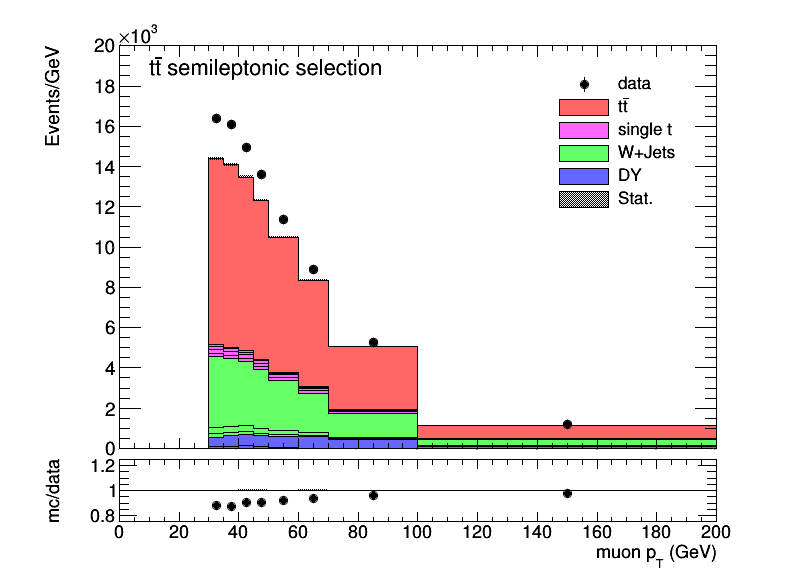
\includegraphics[width=7cm]{assets/semilep_pt.png}}\quad
     \subfigure[]{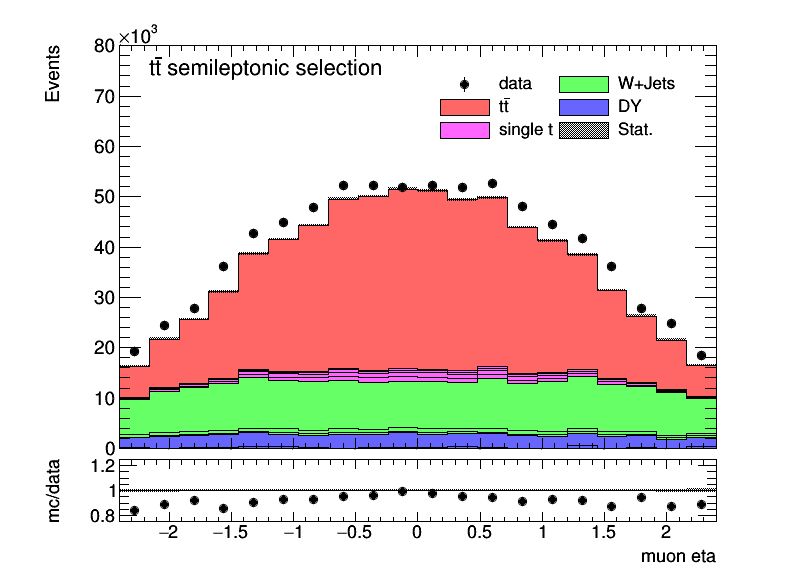
\includegraphics[width=7cm]{assets/semilep_eta.png}}\\
     \subfigure[]{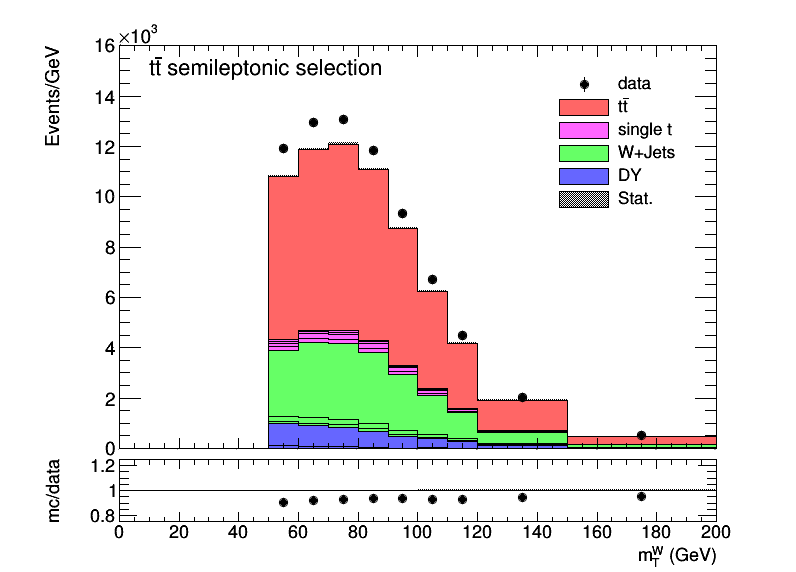
\includegraphics[width=7cm]{assets/semilep_mwt.png}}\quad
     \subfigure[]{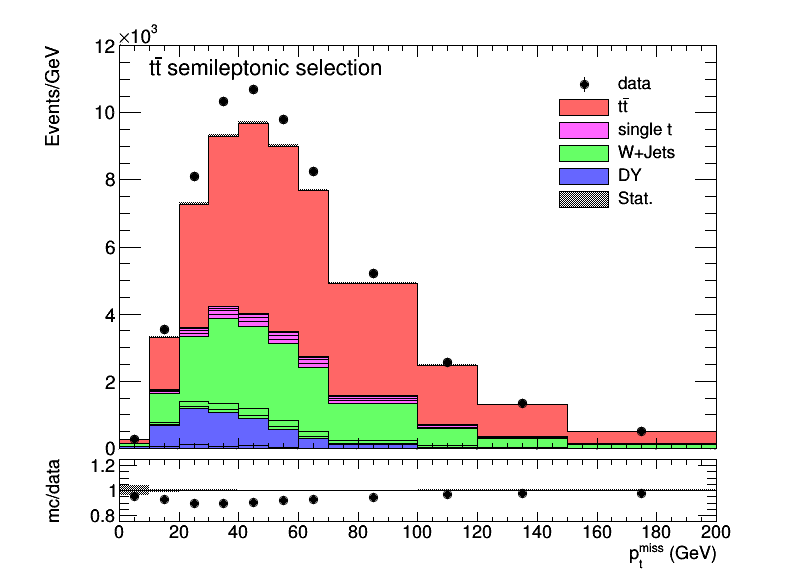
\includegraphics[width=7cm]{assets/semilep_ptmiss.png}}
     
   \end{minipage}\\[1em]
	\caption[Distributions of Variables from the Semileptonic Selection]{\textbf{Distributions of variables from the semileptonic selection.} Shown are the distributions of muon \pt (a), muon $\eta$ (b), reconstructed transverse energy of the W boson $m^\textrm{W}_\textrm{T}$ (c) and the missing transverse energy $\pt^\textrm{miss}$ (d). The total amount of events in data is about 7 \% higher compared to the simulation. The shape in each distribution is in good agreement. The statistic uncertainties are negligible, systematic uncertainties have not been computed.}
	\label{fig:ch_6_semilepDist}
\end{figure}


\section{Top Quark Pair - Dileptonic  Selection} \label{sec:ch_6_dilep}
The dileptonic decay mode can be further distinguished in respect of the leptons in the final state. The decay mode with two muons or two electrons in the final state are dominated by Drell-Yan processes which have mainly additional light flavor quark and gluon jets. The decay mode with a muon and an electron with opposite charge, shown in figure \ref{fig:ch_6_semilep_dilep} has the clearest signal for t$\bar{\textrm{t}}$ and is therefore preferred. The selection criteria are
\begin{description}
\setlength{\itemsep}{-20pt}
\item[•] one good muon with \pt > 20,\\
\item[•] one good electron with opposite charge,\\
\item[•] $M_\textrm{inv} > 20\,\GeV$ of the electron-muon pair to reject backgrounds,\\
\item[•] the good electron or the good muon with $\pt > 25\,\GeV$,\\
\item[•] a trigger selection, which is explained in the following.
\end{description}
The main contributions from other processes are Drell-Yan processes where, for example one muon is misidentified as an electron. Minor contributions coming from vector boson pairs (WW, WZ and ZZ), W boson processes and single top quark processes. 

\begin{figure}
\centering
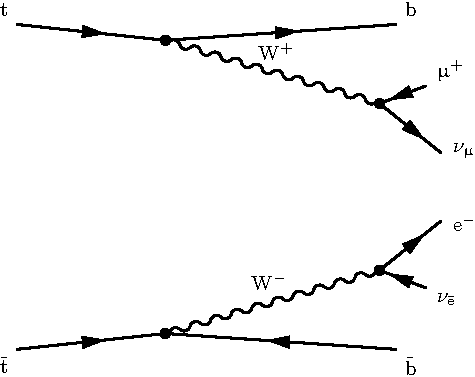
\includegraphics[width=0.4\textwidth]{assets/Feynman/dilep_emu_tt.pdf}
\caption[Dileptonic Decay of a Top Quark Pair]{\textbf{Dileptonic decay of a top quark pair.} With a selection of the muon and electron, a high fraction of t$\bar{\textrm{t}}$ events can be achieved, and therefore many b jets are obtained. Further cuts on the amount of jets or the missing $p_\textrm{T}^\textrm{miss}$ are not necessary for this thesis. Additional jets through initial or final state radiation, pileup or through the parton shower are possible.}
\label{fig:ch_6_semilep_dilep}
\end{figure}

\subsection{Datasets}
The measured events are taken from the muon-electron/photon dataset. Two HLTs were used in the selection where both require one isolated muon and one isolated electron. The first (second) has a limit for the muon of $\pt > 23\,\GeV$ ($\pt > 8\,\GeV$) and for the electron of $\pt > 12\,\GeV$ ($\pt > 23\,\GeV$). Unfortunately there was a problem during the periods of 2016, two different pairs of these HLTs were used. The total recorded luminosity for this dataset was again computed using the \brilcalc tool to a value of $\mathcal{L} = 35.199\,\textrm{fb}^{-1}$.\\

For the simulation, the same datasets were used for the t$\bar{\textrm{t}}$, Drell-Yan, Wt, and W$\bar{\textrm{t}}$ processes. For the W boson with additional jets, the W + jets datasets was used here. Single t and single $\bar{\textrm{t}}$ processes in the t-channel have a negligible contribution and are not included. Instead, processes with two bosons were included, the \pythia 8 program were used for the matrix element generation in NLO and the simulation of subsequent processes. The datasets are given in table \ref{tab:ch_6_Datasets}. 

\subsection{Data-to-Simulation Comparison}
The comparison was done in the same way than for the semileptonic selection in the last section. The fact that two different sets of trigger were used during the periods of the 2016 data has to be taken into account for the simulation. The event weights are therefore additionally multiplied with a flag $f \in \{0,1\}$ of the HLT of the corresponding period. Moreover a trigger for the isolated electron $sf^\textrm{IDandISO}$ has to be included. The event weight is then given by
\begin{equation}
\begin{split}
w_i(nPV,\, p_{\textrm{T},\upmu},\, \eta_\upmu,\, p_\textrm{T,el},\, \eta_\textrm{el},\, &\eta_\textrm{SC,el},\, w_\textrm{lhe},\, f_r) = \frac{\sigma_i}{N_{i,\textrm{gen}}^\textrm{eff}} \cdot w^\textrm{PU}(nPV) \cdot w_\textrm{lhe}\\
 \cdot \sum_{r \in \{\textrm{Periods}\}} \biggl( f_r  \cdot \mathcal{L}_r \cdot &sf^\textrm{ID}_r(p_{\textrm{T},\upmu},\eta_\upmu) \cdot sf^\textrm{Iso}_r(p_{\textrm{T},\upmu},\eta_\upmu) \cdot sf^\textrm{Track}_r(\eta_\upmu)  \\
  \cdot &sf^\textrm{IDandISO}_r(p_\textrm{T,el},\eta_\textrm{SC,el}) \cdot sf^\textrm{HLT}_r(\eta_\textrm{el},\eta_\upmu) \biggr)
\end{split}
\end{equation}
The selection has no requirement of the number of jets. The number of jets together with distributions for the leading (trailing) lepton, which is the good muon or good electron with the highest (lowest) {\pt}, is shown in figure \ref{fig:ch_6_dilepDist}. 



\begin{figure}[!ht]
   \begin{minipage}{\textwidth}
     \centering
     \subfigure[]{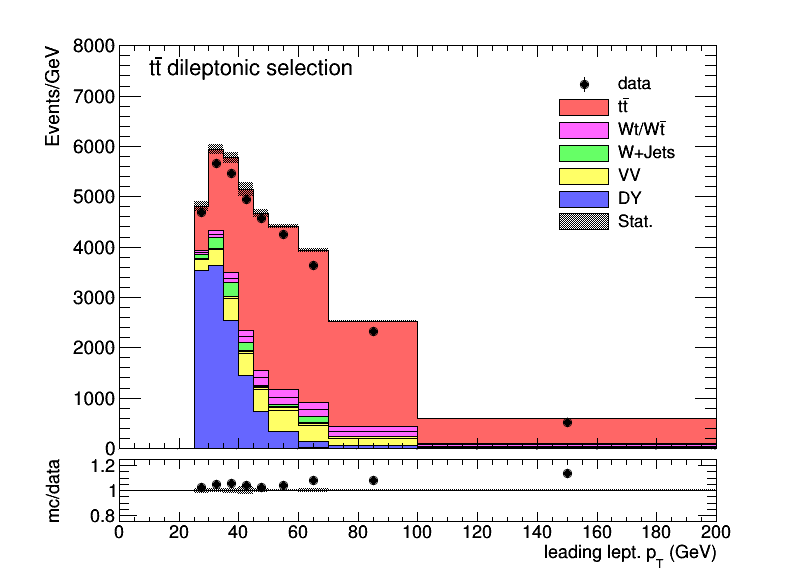
\includegraphics[width=7cm]{assets/dilep_ll_pt.png}}\quad
     \subfigure[]{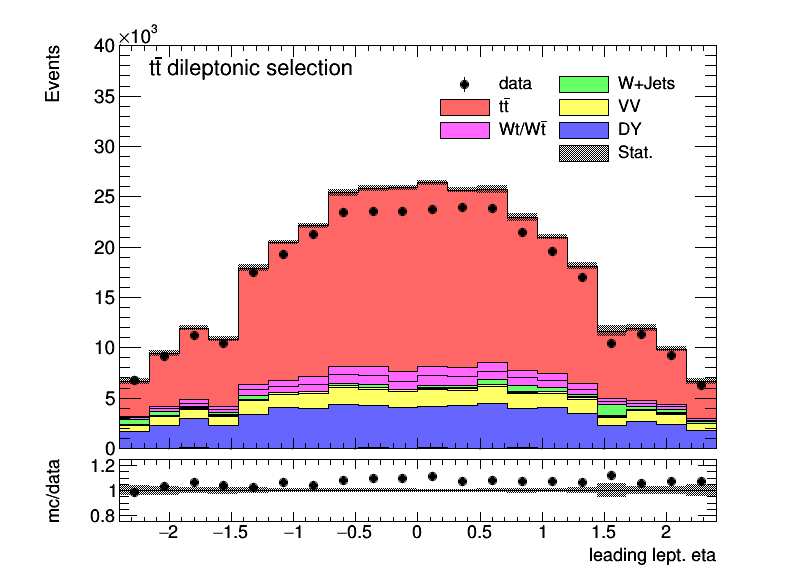
\includegraphics[width=7cm]{assets/dilep_ll_eta.png}}\\
     \subfigure[]{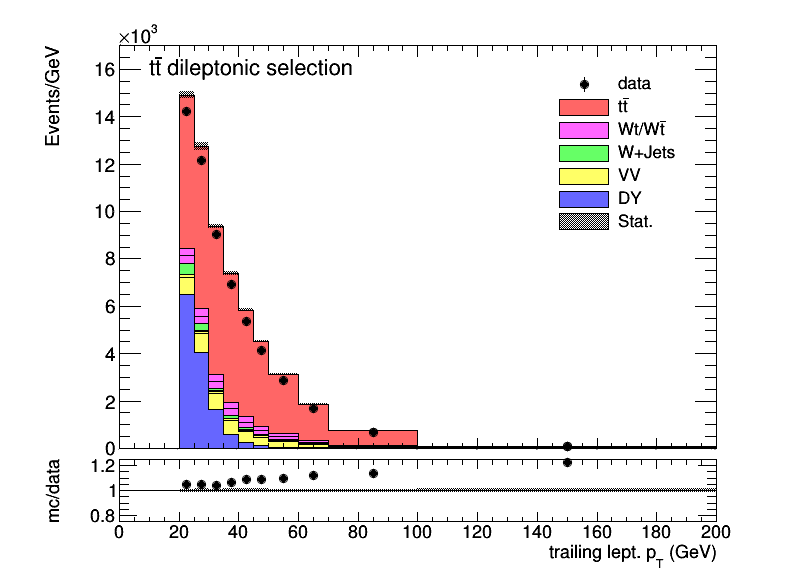
\includegraphics[width=7cm]{assets/dilep_tl_pt.png}}\quad
     \subfigure[]{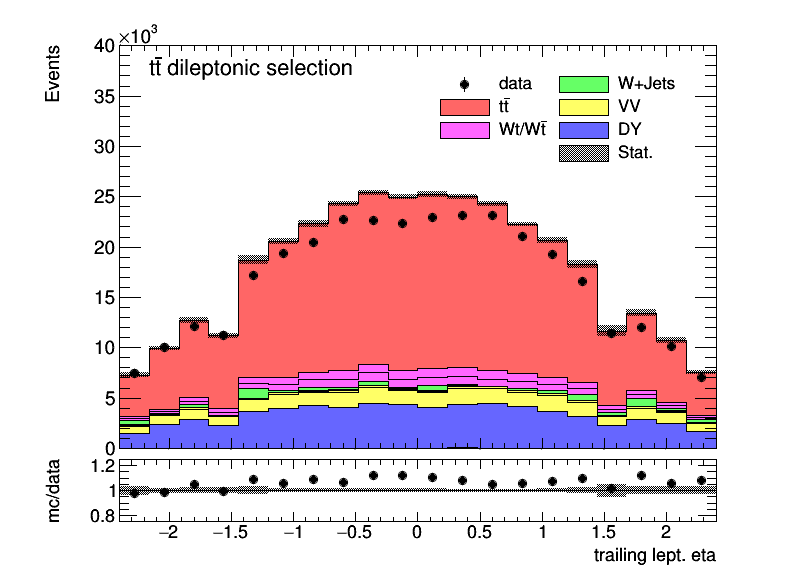
\includegraphics[width=7cm]{assets/dilep_tl_eta.png}}\\
     \subfigure[]{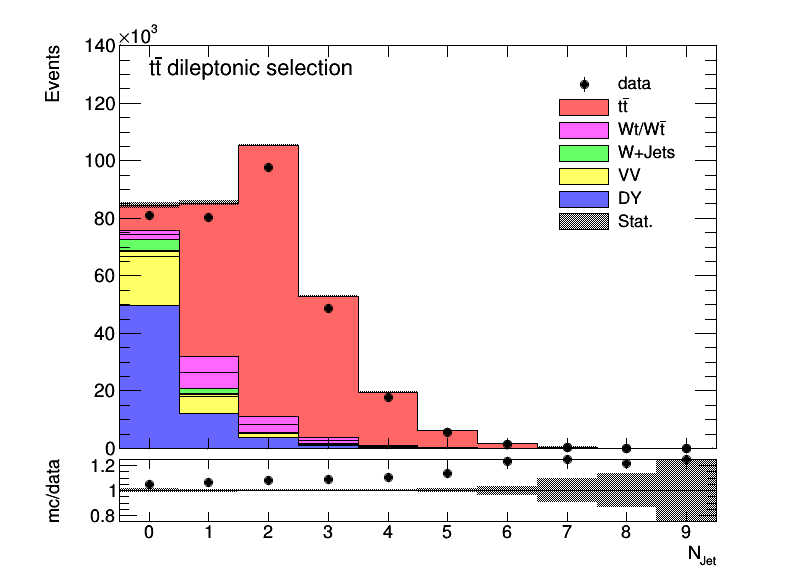
\includegraphics[width=7cm]{assets/dilep_njets.png}}
     
   \end{minipage}\\[1em]
	\caption[Distributions of Variables from the Dileptonic Selection]{\textbf{Distributions of variables from the dileptonic selection.} Shown are the distributions of \pt (a) and $\eta$ (b) of the leading lepton, and the \pt (c) and $\eta$ (d) of the trailing lepton and the number of jets (e) in each event. The number of simulated events is about 7 \% higher than the number of events in data. The reason is assumed in wrong scalefactors. However the shape is again in a good agreement. The statistical uncertainties are higher but still negligible, the systematic uncertainties are not given.}
	\label{fig:ch_6_dilepDist}
\end{figure}

\chapter{Domain Adaptation Studies}

\section{Domain Adaptation on the DeepFlavour Algorithm}

\subsection{•}

\section{Domain Adaptation on the DeepCSV Algorithm}

\section{Two Tag Efficiencies}


\include{conclusions}

\appendix
\include{appendix/appendix_a}
\include{appendix/appendix_b}
\include{appendix/appendix_c}
 
\listoftables
\listoffigures

\bibliographystyle{includes/custom2}

\bibliography{references}
\backmatter
 
\end{document}
